\documentclass[9pt]{report} 
\usepackage[paperwidth=15.24cm, paperheight=22.86cm]{geometry}
\usepackage[pdftex]{graphicx}
\usepackage{setspace}
%\usepackage{lineno}

%\usepackage[letter,frame,center]{crop}

\usepackage{color}
\usepackage{float}
\usepackage{enumitem}
\usepackage{listings}
\lstset{basicstyle=\small\ttfamily,breaklines=true,backgroundcolor=\color{lightGrey}}

%\usepackage{bbm}
\usepackage{hyperref}
\usepackage{lscape}
\definecolor{PiranaOrange}{rgb}{0.9,0.4,0.1}
\definecolor{Blue}{rgb}{0.0,0.0,0.7}
\definecolor{Red}{rgb}{0.7,0.0,0.0}
\definecolor{Grey}{rgb}{0.4,0.4,0.4}
\definecolor{Grey}{rgb}{0.4,0.4,0.4}
\definecolor{LightGrey}{rgb}{0.92,0.92,0.92}
\definecolor{grey2}{rgb}{.92, .92, .92}

\bibliographystyle{unsrt}%Choose a bibliograhpic style}
%\usepackage{utopia} %\usepackage{charter} %\usepackage{palatino}
%\usepackage{bookman} %\usepackage{newcent} %\usepackage{times}
%\usepackage[options]{natbib} \sloppy

% font
%\renewcommand{\familydefault}{\sfdefault} 

\usepackage{mathpazo}
\renewcommand{\familydefault}{\rmdefault}

%\oddsidemargin 1.5cm
%\textwidth 13cm
\textheight 17.5cm

\newcommand{\test}{\textcolor{Blue}{\textit{test}}\xspace}
\newcommand{\reference}{\textcolor{Green}{\textit{reference}}\xspace}
\newcommand{\valpsn}{\textcolor{Blue}{\textit{valpsn}}\xspace}
\newcommand{\ValPsN}{\textcolor{PiranaOrange}{\textit{ValPsN}}\xspace}
\newcommand{\psn}[1]{\textcolor{Grey}{#1}}

\newcommand{\fname}[1]{\textit{#1}}
\newcommand{\action}[1]{\textcolor{Red}{\textit{#1}}}
\newcommand{\command}[1]{{\ttfamily{#1}}}

%% code listings
\lstset{
  language=fortran,                   % the language of the code
  basicstyle=\ttfamily\small,    % the size of the fonts that are used for the code
  commentstyle=\color{Grey}\textit,
  backgroundcolor=\color{LightGrey},  % choose the background color. You must add \usepackage{color}
  captionpos=b,                       % sets the caption-position to bottom
  columns=flexible,
  showspaces=false,
  showstringspaces=false,
  showtabs=false,
  morekeywords={*, ...}               % if you want to add more keywords to the set
}

\begin{document}

\title{
  \vspace{-100pt}
  \textbf{
  \textcolor{PiranaOrange}{\Large Pirana}
  }\\
  \vspace{5pt}
  \small \textcolor{Grey}{Pharmacometrics workbench for NONMEM \& PsN} \\
  \normalsize
  \vspace{15pt}
  \hspace{15pt}
\includegraphics[scale=0.2]{images/pirana_logo.jpg}\\
  \vspace{15pt}
  \small Installation guide\\Manual\\Tutorial\\Quick Guides\\
  \vspace{8pt}  \textit{Pirana version $\geq$ 2.10.0}\\
  \vspace{8pt}
%  \scriptsize {\today} \\
  \date{}
}

\maketitle

\null\vfill
\noindent

\vspace{5pt}

\small
\noindent Creative Commons Attribution-NonCommercial-ShareAlike 4.0 International License. -- Pirana Software \& Consulting BV\\

\vspace{5pt}

\noindent Chapter 9, the tutorial on Pirana, PsN, and Xpose, has
earlier been published in the open access journal CPT-PSP (Nature
Publishing Group).  This chapter is available under a creative commons
license (Commons Attribution-Noncommercial-No Derivative Works
3.0). In short, this means that you may reproduce the content for
non-commercial purposes, although you are required to attribute its
authors, and may not alter the content.

\normalsize

\newpage

\tableofcontents
\newpage  % one page left blank intentially
\thispagestyle{empty}
\mbox{}

%%%%%%%%%%%%%%%%%%%%%%%%%%%%%%%%%%%%%%%%%%%%%%%%%%%%%%%%%%%%%%%%%%%%%%%%%%
%!TEX root = manual_booklet.tex

%%%%%%%%%%%%%%%%%%%%%%%%%%%%%%%%%%%%%%%%%%%%%%%%%%%%%%%%%%%%%%%%%%%%%%%%%%
\chapter{Introduction} Pirana is a powerful
modeling environment for NONMEM, PsN and Xpose, offering a graphical
user interface and many auxiliary tools to support modeling \& simulation analyses.\\

\noindent Development of Pirana was started in 2007 as an open source
project. As of version 2.4.0, Pirana is released under a commercial
license for non-academic users, while it is released (free of charge)
under a Creative Commons license for academic users. Pirana is
designed to be very flexible, and extendible: it integrates
with many existing software such as R, Excel, and Berkeley Madonna, and it runs on all major operating systems.\\

\vspace{1pt} \noindent We attempt to make Pirana as intuitive as
possible, but reading this manual before or while you start working
with Pirana is recommended. For many
common functionality in Pirana, a Quick Guide is available (from
Pirana's help-menu, or from www.pirana-software.com). Also have a look at our website for more information and an FAQ. If you're still in the dark at some point, please do not hesitate to contact us.

\vspace{20pt}

\noindent \scriptsize{info@pirana-software.com} \normalsize


\pagebreak

\newpage  % one page left blank intentially
\thispagestyle{empty}
\mbox{}

%%%%%%%%%%%%%%%%%%%%%%%%%%%%%%%%%%%%%%%%%%%%%%%%%%%%%%%%%%%%%%%%%%%%%%%%%%

\chapter{Pirana installation}

Software requirements are summarized below, followed by some additional details on the installation procedure.

\section{Required / recommended software}

Although the only real requirement is an installation of NONMEM, some additional software is highly recommended for optimal use of Pirana, while other softwares might be useful as well.

\begin{description}
\item[\textcolor{Red}{NONMEM}] Pirana can use both standard
  `from-CD'-installation of NONMEM and NMQual NONMEM
  installations. NONMEM doesn't have to be installed on your local PC,
  since Pirana can also connect to other PCs or clusters.

\item[\textcolor{Blue}{PsN}] Strictly, Pirana does not require PsN
  installed, although the PsN-toolkit is highly recommended. The latest
  version of PsN can be obtained from \textcolor{Grey}{http://psn.sourceforge.net/}.

\item[\textcolor{Blue}{Xpose}] This R-package for model diagnostics is
  highly recommended and can be obtained from
  \textcolor{Grey}{http://xpose.sourceforge.net}. Xpose datasets can
  be selected and loaded in R/Xpose, and an Xpose GUI is available
  within Pirana.

\item[\textcolor{Blue}{R}] This open-source software can be
obtained from \textcolor{Grey}{http://www.r-project.org/}, and is highly
recommended for optimal use of Pirana. R Studio
(\textcolor{Grey}{http://www.r-studio.org/}) is a powerful GUI for
R that works well with Pirana.

\item[\textcolor{Grey}{WFN}] Not required/recommended. Pirana offers only basic
  support for Wings for NONMEM. 

\item[\textcolor{Grey}{NMQual}] Recommended for keeping an audit trail of NM
  installations and autamatically performing bug-fixes. Pirana
  supports the use of NMQual NONMEM installations. NMQual also
  requires Perl and the module XML::XPath installed. More details can
  be found at the Metrum website
\end{description}

\section{Installation}

\subsection{Installation procedure on Windows} Download the installer
from the Pirana website, and install to any location on your hard-drive. Before exploring
Pirana's functions, you should first check your settings ('File
$\rightarrow$ Settings $\rightarrow$ General...') and software
integration ('File $\rightarrow$ Settings $\rightarrow$ Software
locations...'). If you want to connect to clusters, also update the
`Cluster' settings.  Pirana is tested on XP, Vista, 7, and 8. Upon installation, 
Windows may complain that installation is not safe, but this warning can be ignored.

\subsection{Installation procedure on Mac OS X} On Mac, you should
first install the Xcode tools, which are
included as optional installs on the (Snow) Leopard install DVDs. In the most recent OSX versions, Xcode can be installed from the App Store. After installing Xcode, make sure you also install the Command Line Tools (From within Xcode, go to `Preferences', and `Downloads'). Secondly you will have to install an X-window manager (either X11 or XQuarts). For old versions of OSX, X11 is most likely already installed. If you are running Lion or later, you will however have to install XQuartz instead of X11, which is downloadable online (google for `XQuartz'). Pirana for Mac is distributed as an executable, so no Perl installation is required, but it is also possible to run from source (see Linux explanation). When opening Pirana for the first time, your system may complain that Pirana is not safe, since it is not installed from the App Store. In this case, you will have to set your security settings in your systems `Preferences' to run apps from `Everywhere', instead of from `App Store only'.

\subsection{Installation procedure on Linux} For Linux, an executable
is made available as well. This executable is compiled on a 32-bit
system. If for some reason this executable doesn't run on your system,
the Perl source-code can be executed directy in Perl. This requires
manual installation of a few additional libraries and modules, see below.

\subsubsection*{Installing Perl and X11 development libraries}
For Pirana to be able to create the GUI, the X11 development libraries
(libX11-dev) should be installed, as well as the Perl/Tk module. In
Ubuntu / Debian, you can use the Synaptic package manager to install
these, or using apt from the shell:

\begin{lstlisting} 
sudo apt-get install libX11-dev perl-tk
\end{lstlisting}

\subsubsection*{Installing additional Perl modules}
\noindent Pirana makes use of a number of publicly available
Perl-modules, which should also be installed. Some of these modules
are likely to be already installed with you current Perl distribution,
while others have to be installed manually. Below is a short guidance
on how to install these modules. Further guidance on installing Perl
modules can be found here: \textcolor{Blue}{
  http://www.cpan.org/modules/INSTALL.html}). To make a connection to
the Perl module archive (CPAN), type:

\begin{lstlisting} 
sudo perl -MCPAN -e shell
\end{lstlisting}

\noindent The following commands may be needed to set up the CPAN
shell to be able to correctly `make' the modules into your Perl distribution.
\begin{lstlisting}
o conf make /usr/bin/make
o conf make_install_make_command 'sudo make'
o conf commit
\end{lstlisting}

\noindent Next, use the `install' command to install required modules
into your Perl distribution (mind the case-sensitivity for the module
names). Look in Some of these may already be installed, which will be reported
as such. If you cannot install some modules from CPAN directly, you
have to download and install these modules (and their
dependencies) manually. Look in the file pirana.pl to see which
modules to install (this may change between Pirana versions).

\begin{lstlisting}
install Tk::PlotDataset
install Tk::JComboBox
install ...
\end{lstlisting}

\noindent Some required modules cannot be installed directly from
CPAN. These modules are supplied with Pirana (in the folder
`/packages') and should be installed manually. From within each of the
two package folders, execute in a shell:

\begin{lstlisting}
perl Makefile.PL
make
sudo make install
\end{lstlisting}

\vspace{8pt}
\noindent\scriptsize{\textcolor{Blue}{Note:} \textcolor{Grey}{Checking
whether Perl modules are installed correctly can be done by executing the
following in the terminal window, e.g.: perl -e 'use Tk' which should
result in no error messages.\\ } } \normalsize

\subsubsection*{Pirana installation}
\noindent After installing these Perl modules, copy the entire pirana
folder contained in the zip-file to e.g. your home folder
(/home/username/) or /opt/pirana/ if you are system
admin. Make sure that all perl files in that folder have
execution rights. To grant these rights to yourself you can execute
the following in the shell from within the Pirana folder:

\begin{lstlisting} 
sudo chmod 711 -R *
\end{lstlisting}

\subsubsection*{Pirana execution}
\noindent Pirana can now be started from the command line using

\begin{lstlisting}
perl pirana.pl
\end{lstlisting}

\noindent from within the Pirana folder. Pirana was tested on Ubuntu
(9.04-12.04), OpenSUSE (11.1), and Arch Linux, with Perl
distribution 5.10.0 or lower. Pirana should work on any Linux distribution
with X-windows and Perl/Tk installed.

\section{Installation of license file} License files can be installed by going to `Help' $\rightarrow$ `Import license file'. On Windows, you can also install the license file by dropping it on the Pirana main window. Upon starting Pirana, the presence of a valid license file (pirana.lic) in Pirana's main installation folder will be checked. If no valid license file is present, a message will be displayed and some functionality of Pirana will be
disabled. Academic, commercial, or trial license files can be obtained
on the website. 

\section{Configuration} Although most preferences will
be correct by default, we recommend to check at least the
settings detailed below. Familiarize yourself with
the other options as well, to get the most out of Pirana. Especially check the correct file extensions
for NONMEM model files and output files.

\begin{description}
\item[File extension of models] NONMEM control streams/model files. Default is .mod. Note that multiple
model file extensions can be specified separated by a comma, e.g. `mod,ctl'. 
\item[File extension of results] NONMEM output. Default is .lst

\item[Software settings] Pirana needs to know where other important software is installed,
which is specified under `Software' from the `File' menu. References
to software that you do not have installed, may be disregarded as they
are ignored by Pirana.

\item[Code editor] Preferably an editor syntax-highlighting. We
  recommend the use of Emacs (all OS), PSPad (Windows), ConTEXT (Windows), Sublime Text 2 (MacOSX). If none is
  entered, or a non-existing program is specified, Pirana will use its
  built-in NM-TRAN editor.
\item[R location] The location (folder) of R, e.g. C:/Program
  Files/R/R-2.11.0. On Windows, at first start-up of Pirana it will
  search for the latest version of R that is installed, and
  automatically updates this setting accordingly. If R is installed in
  a non-standard location, please update this.
\item[R GUI] The GUI to be used for R-scripts. Recommended for this is
  RStudio or Emacs/ESS, but the RGUI supplied with the R distribution
  can also be used.
\item[spreadsheet] The location of your spreadsheet application,
    e.g. Excel or Gnumeric. Pirana tries to find your spreadsheet
    automatically.
\end{description}

\vspace{10pt}
\noindent\scriptsize{\textcolor{Blue}{Note:} \textcolor{Grey} {on Mac OSX you can either specify the application name
(e.g. "Microsoft Excel"), or the actual location of the application
(e.g. "/usr/local/bin/emacsclient").}
\normalsize

\newpage

\section{Configuration for modeling groups}
IT admins that want to distribute Pirana to a modeling group with
pre-specified settings can do so by editing the files in the folder \textit{ini\_defaults}
before distributing Pirana. This will allow users to start with appropriate defaults for Pirana's setting. Also, one
or more clusters can be added by default, so that users do not have to
add these themselves (and only have to update their username and login). Look in
the file /ini\_defaults/clusters/readme.txt for further
information.

\subsubsection{Configuration files location}
If even more control is required, i.e. if the end-user should not be
allowed to change part of the configuration at all, it is possible to
change the location of the configuration files from the user's home
directory to a different, protected shared location. The default location for
Pirana's configuration files can be overriden by using the file
\textit{ini\_locations.ini} located in the folder where you installed
Pirana. Change the central ini-files rights to read-only, to be sure users do
not change the central settings. More information about how to use
this functionality is available in the annotated \textit{ini\_locations.ini}
file itself.

\newpage  % one page left blank intentially
\thispagestyle{empty}
\mbox{}

%%%%%%%%%%%%%%%%%%%%%%%%%%%%%%%%%%%%%%%%%%%%%%%%%%%%%%%%%%%%%%%%%%%%%%%%%%
\chapter{Using Pirana}

\section{Overview}

\subsection{Basic functions} The Pirana window consists of a large
area showing an overview of models in the current folder, and a
smaller area on the right. The main overview acts as an `electronic lab-notebook' for 
modeling analyses. The list on the right shows e.g. data files, R-scripts,
Xpose datasets, or all files in the active folder, or alternatively a
list of parameter estimates or reports. Most buttons in Pirana's main
screen are accompanied by a short description which is displayed if
hovered above with the mouse pointer. Some specific functionality is
detailed below. By selecting a model or (data-) file in either lists
and right-clicking the mouse, a menu with actions on models or run
results is shown. Most of Pirana's functionality is available from
this menu, and most options are also available from the toolbar
(\textit{View} $\rightarrow$ \textit{Show toolbar}).

\begin{figure}[H] \centering
    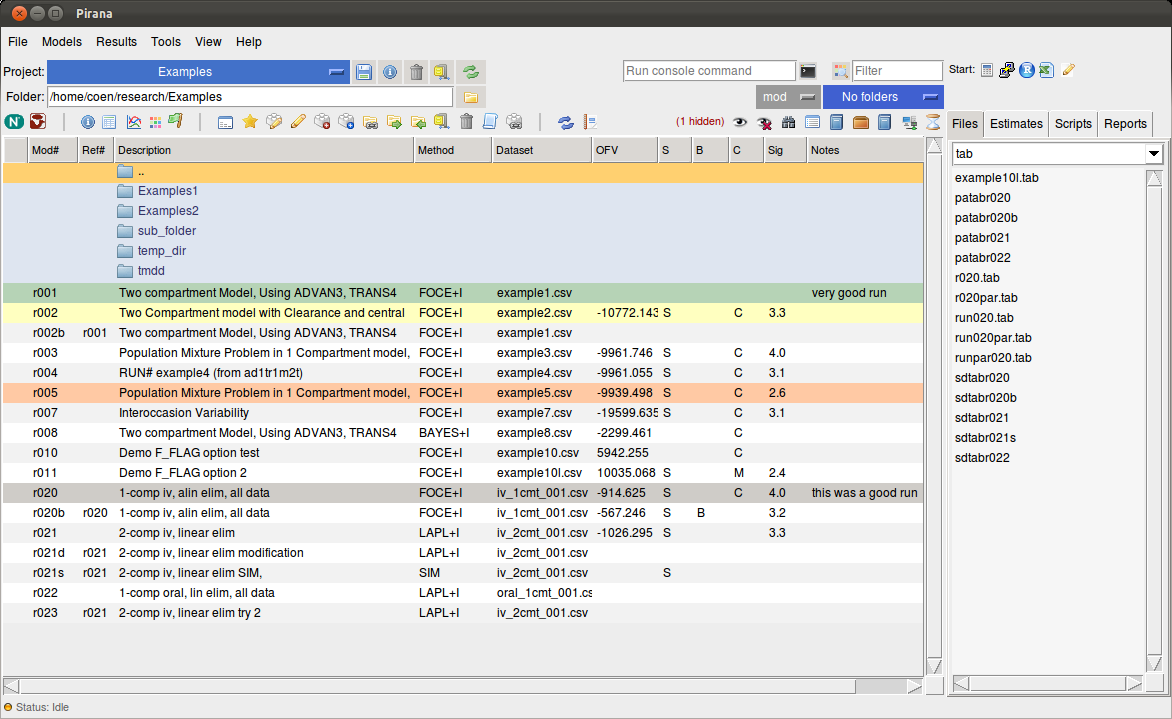
\includegraphics[scale=0.25]{images/pirana_main_screen.png}
    \caption{Pirana main screen (on Linux)}
\end{figure}

\subsection{Model management} The main model overview is 
where all models and subdirectories in the current working directory
are displayed. Only models are displayed that have a file-extension
corresponding to the file extension specified in the
\textit{preferences}. If multiple file extensions were specified, choose the
one you want to use in the current folder by selecting it from the listbox 
(the one next to the folder selector, on the right above the main models list). 
When models are double-clicked, the control stream is opened in the
code-editor (if specified), or else in Pirana's built-in NM-TRAN
editor.

\subsubsection*{Model views}
By default, the model overview is shown as a list, listing all models
ordered by run number. It is assumed models are named as a number
(e.g. '001.mod'), or prepended with 'run' (e.g. `run1.mod', or 'run001.mod'), see
`Conventions and Methods' for more information. By default, the list is shown in \textit{condensed mode},
meaning that for every model, a single row is used in the table. The
list can however also be shown in \textit{expanded mode}, which allows
for longer model descriptions and notes in the overview. Additionally,
in this mode all estimation methods are shown, while in condensed mode
only the last estimation method and associated OFV is shown.

An alternate view mode is \textit{tree view}, in which model development is
shown as a hierarchical tree. The tree is built using parent/reference
information included in the model files (see `run record' explanation in this manual). When creating models in Pirana, this information is added automatically, and adheres to PsN's run record syntax. 

The columns that are shown in the main overview can be activated or de-activated from the \textit{View} $\rightarrow$ 
\textit{Show columns} menu. Models can be filtered using the `Filter' above the
main overview table, or by colors or flags.

\subsubsection*{Model actions}
\noindent New models can be created from scratch, from a template, by
using the Wizards, or by duplicating an existing model:

\begin{description}
\item[Wizards]\ Models can be created by using the PK model
wizard. Choose the desired model type and estimation method, and a
basic NONMEM model file will be created.

\item[Templates] Many basic template models are included. It is
possible to build your own library with base models that you often
use. Templates can be added by copying a model file to
\ttfamily{/templates }\normalfont in the Pirana directory. The
template models should have the same file extension as your model
files to be recognized as a template.

\item[Duplication] Duplication of models can be performed by
selecting the parent model and clicking `duplicate' from the
context-menu (right click on the model). Optionally, final parameter estimates
from the reference model can be updated in the new model, and also
model-file numbers in \$TABLE and \$EST records. Some basic syntax
rules should be adhered to ensure correct interpretation of final
estimates, see Conventions and Methods at the end of this chapter. A
model can also be \textit{Duplicated for MSF restart}. This means that the
model file is duplicated, but an \$MSFI record is added, parameter
estimate blocks are commented out, and the \$MSFO record is updated.

\begin{figure}[H] \centering
    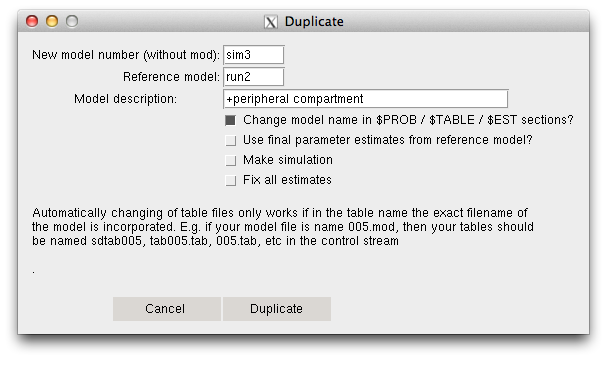
\includegraphics[scale=0.4]{images/duplicate.png}
    \caption{Duplicate model}
\end{figure}

\end{description}

\subsubsection*{Notes, flags and colors}
To each model / run in Pirana, notes can be added. Also, flags and
colors can be added, indicating \textit{key runs}, \textit{good runs},
or \textit{bad runs}. Of course the meaning of the flags and
color-coding is all up to the user. The notes and color info are
stored in a database file (\textit{pirana.dir}), which is created
automatically in each folder that holds models. To add notes to a
model, select the model, right click and select \textit{Model}
$\rightarrow$ \textit{Notes and info}, or using the \textit{Ctrl-I} shortcut. Models and results can be given a color by selecting the model, right-clicking, and selecting the desired color/flag from the \textit{Colors \& flags} submenu. Tip: Pirana supports filtering of models/runs by color.

\vspace{8pt}
\noindent
\scriptsize{
\textcolor{Blue}{Note:} \textcolor{Grey}{In each active folder that
    is visited with Pirana, a small SQLite database is created
    (`pirana.dir') which is able to store information about models. So
    if you archive your projects manually, make sure to include these files as
    well.  }
}
\normalsize

\subsection{Projects} Pirana allows you to save a link to a folder as
a project, which will then be shown in the blue bar (above the active folder
entry). This allows you to quickly switch to the directory that is
linked to that project. To add a project to the list, browse to a
folder by clicking on the folder-icon next to the location bar, or by
clicking through the directory-listing in the model overview. Next,
click on the \textit{disk}-icon next to the project name, give your
project a unique name and press `Save'. Your project is now available
from the listbox. To delete a project from the list, click the trash
icon next to the project list. The green refresh-icon refreshes the
view of the current directory, and should be applied when you make
changes to models or add files outside of Pirana. Also when a run is
finished, you should refresh to gather the results into Pirana.


\subsection{Data files} The list on the right of the screen shows
files in the current folder, if `Files' is selected as the active tab. Pirana can show tab-files, csv-files, R scripts, Xpose files, and other files, which can be selected from the list above. It is also possible to specify your own
filter. Right-clicking on a selected file shows a menu with possible
actions on the file.

\vspace{8pt}
\noindent\scriptsize{\textcolor{Blue}{Note:} \textcolor{Grey}{When the
    Xpose option is chosen, only unique run numbers are shown, instead
    of all tabualar data files. After selecting an Xpose dataset,
    click the `Open in R' the right-click-menu, and R read in the
    datasets and create the Xpose object.  } \normalsize

\section{Working with NONMEM}

There are several ways in which NONMEM can be used from Pirana. The
first one is to use the nmfe-script supplied with NONMEM. For this,
you have to instruct Pirana where NONMEM is installed. The other
(recommended) way to run NONMEM, is to use PsN. When you run NONMEM
through PsN, you don't have to tell Pirana where NONMEM is located,
since this is already specified in the \textit{psn.conf} file of PsN.

\subsection{Managing NONMEM installations} Existing NONMEM
installations can be added to Pirana via the Settings menu, under the
NONMEM tab. Here, both local (upper) and cluster (lower) installations
can be added for use in Pirana. A \textit{smart search} tool is implemented
for local NONMEM installations, which searches for NONMEM
installations in the most common locations on your local drives. If
you have installed NONMEM in a non-common location, or want to use
NONMEM on a remote cluster, add the paths to NONMEM manually.

\begin{figure}[H] \centering
    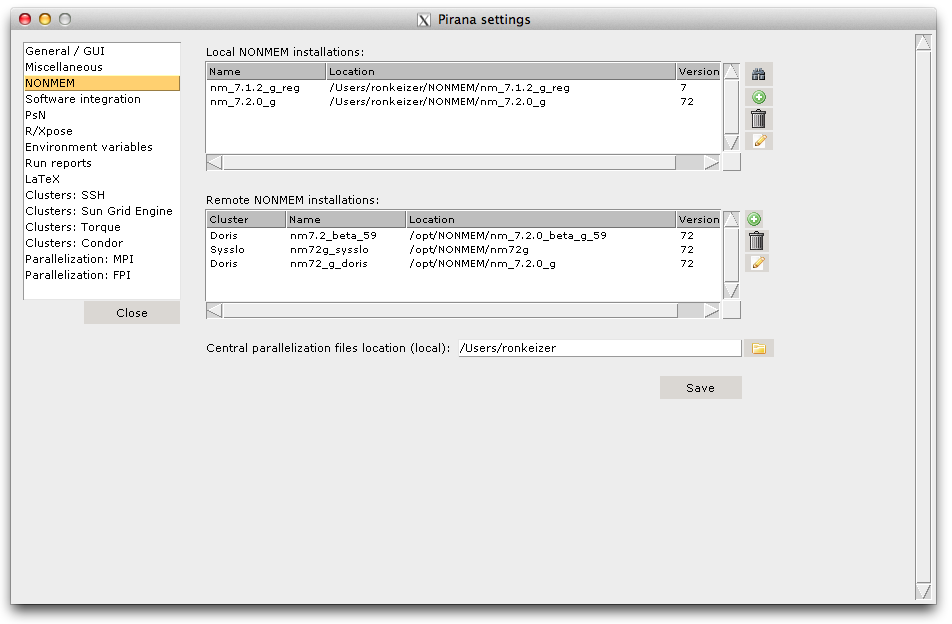
\includegraphics[scale=0.31]{images/nonmem_settings.png}
    \caption{NONMEM settings window}
\end{figure}

\subsection{Setting environment variables}
NONMEM requires a Fortran compiler installed. For
this compiler to function properly, it is important to set the
environment variables correctly. Especially for Intel compilers, this
can be trooublesome, as different environmental variables need to be
defined. For GNU compilers, setting the PATH environment variable is
usually sufficient. There are several ways you have control over the
environment variables when using Pirana:

\begin{enumerate}
\item In the settings menu, under \textit{Environmental variables},
  the PATH variable used within the Pirana environment can be defined,
  or additional folders can be added to the existing PATH. Also,
  additional environmental variables can be defined here.

\item Alerntatively, in the same settings screen for each nmfe-run
  that is started, you can specify a command that will be executed
  before starting nmfe-type runs, which can be e.g.

\begin{lstlisting}
  PATH=%PATH%;C:\gfortran\bin
\end{lstlisting}

\item At startup, Pirana will check for the existence of 2 files in
  the Pirana base folder: \textit{set\_env.txt} and
  \textit{add\_env.txt}. These files can be used to either set, or add
  to the system variables, respectively. The files may look e.g. like
  this:

\begin{lstlisting}
PATH=C:\nmvi\run;C:\MinGW\bin
VARX=C:\bladibla;etc
\end{lstlisting}
\end{enumerate}

\clearpage
\subsection{Running models}
As mentioned before, a model can be run using \textit{nmfe} directly, \textit{PsN} or
\textit{WFN} (Windows only). This can be done by selecting a model from the list, and
right-clicking to show the context-menu.  From here, you can either
select NONMEM-nmfe, or the PsN or WFN options. The commands are also
available from the toolbar. WFN is disabled by default.

\subsubsection*{Using nmfe}
Execute a model using `Run (nmfe)', or press Control-R. This will open up a
dialog showing two additional options
for running the model, e.g. which NONMEM installation to use, and if
models should be executed in separate folders or on a cluster system.

\begin{figure}[h] \centering
    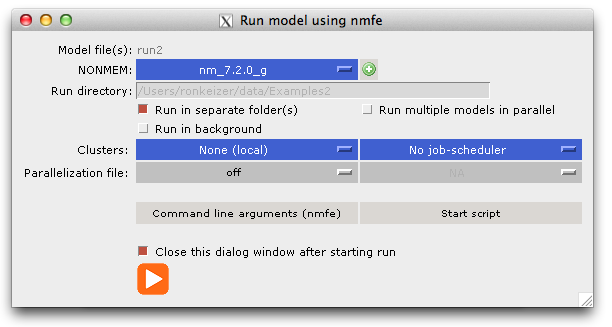
\includegraphics[scale=0.5]{images/nmfe_run.png}
    \caption{nmfe run window}
\end{figure}

\noindent Pirana supports the use of the parallelization functionality available
in NONMEM 7.2. When you select a NONMEM 7.2 installation in the nmfe
run window, the available parallization files (\textit{parafiles}) are displayed under the parallelization tab. \textit{Parafiles} can be generated using the Wizard in Pirana. You can also have Pirana generate the \textit{parafile} on-the-fly (select \textit{auto-MPI} or \textit{auto-FPI}). Under Settings $\rightarrow$ Parallelization, the FPI and MPI files that Pirana generates can be specified.

\vspace{5pt}

\noindent Parallization files can be imported from local or remote locations. Local import can be performed through Settings $\rightarrow$ NONMEM. Remote parallelization files can be imported from a cluster location defined under Settings $\rightarrow$ SSH.

\begin{figure}[H] \centering
    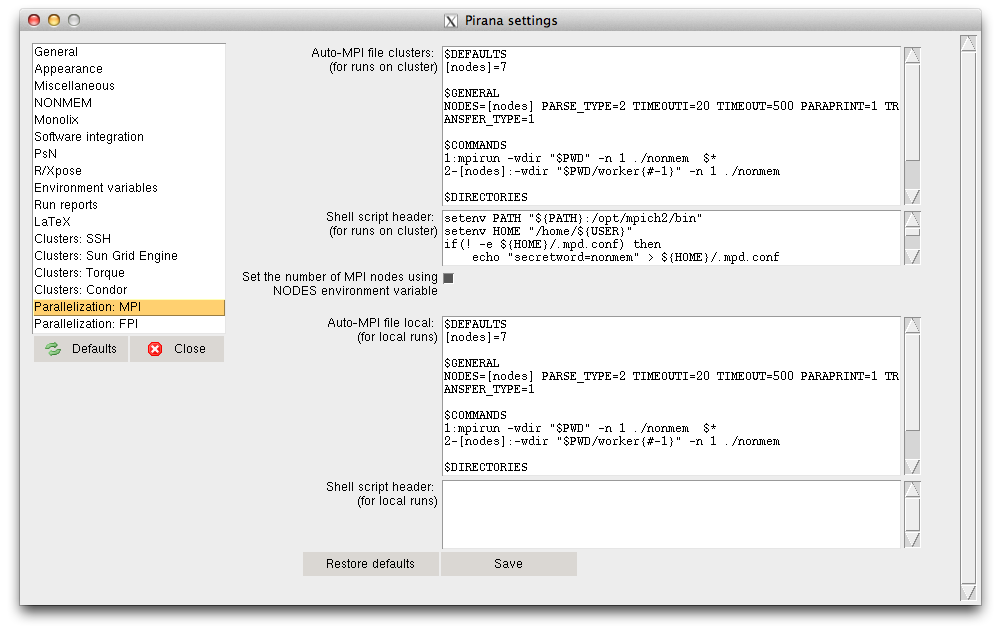
\includegraphics[scale=0.27]{images/settingsparallization.png}
    \caption{Automatic parallelization file}
\end{figure}

\clearpage

\subsubsection{Using PsN}
PsN is an extensive toolkit for advanced modeling \& simulation, and
contains essential tools such as bootstrapping, visual predictive
checks (vpc), stepwise covariate modeling (scm), simulation and
re-estimation (sse), and many more. All PsN-toolkit functions can be
accessed from Pirana using the right-click menu or the toolbar. \textit{Execute} is
also conveniently available using the Ctrl-e keyboard shortcut. The
dialog window is then opened (shown below), which can also shows the
PsN-help info for the selected command. The command line editor can be
used to specify additional parameters to the PsN funtion. Pirana
stores each executed PsN command, which are available from the
'History' button.

\begin{figure}[H] \centering
    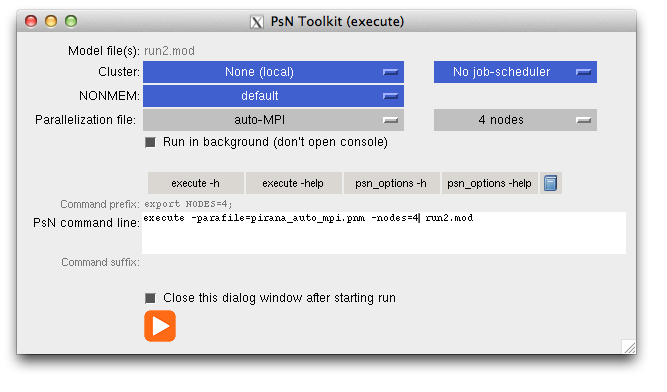
\includegraphics[scale=0.42]{images/Figure2_4_PsNdialog2.png}
    \caption{PsN dialog window}
\end{figure}

\noindent From the PsN tab in the Settings window you can define the default
command line parameters for most PsN functions. Some of PsN's functions are not related to models, but to datasets, such as data\_stats, \textit{create\_subsets} etc. These functions can be invoked from the file list on the right by selecting a file and opening the menu by right-clicking the mouse. A similar interface will be opened
as for PsN's model functions.

Similar to the nmfe dialog window, the PsN dialog also offers the possibility to 
easily setup parallel execution. Pirana can be instructed to auto-generate
the MPI/FPI file required for parallel execution. When MPI or FPI, and the number of nodes are selected,
Pirana will automatically add the required PsN arguments ({\tt -parafile} and {\tt -nodes}).

\subsubsection*{Using Wings for NONMEM} 
On Windows, Pirana is
capable of invoking the WFN-commands \emph{nmgo} and \emph{nmbs}, for
run execution and bootstrapping respectively. Since
WFN does not support multiple model files to be processed by its
commands, when multiple models are selected, only the first model file
is executed. When the WFN method is selected, two parameter
specification bars will become visible. In the upper entry, run
parameters can be specified, e.g. for the bootstrap: `1 100' to
specify a bootstrap with 100 replicates. The lower parameter bar
specifies command-line parameters used when starting WFN.bat,
e.g. `g77 std' for specifying the compiler and the NONMEM version to
be used. 

\vspace{10pt}
\noindent\scriptsize{\textcolor{Blue}{Note:} \textcolor{Grey} {What Pirana actually does when executing runs through WFN, is create a temporary batch-file in the current directory that starts \emph{WFN.bat} to load the necessary environment variables, after which \emph{nmgo} is started with the model-file and parameters specified.}
  \normalsize

\clearpage
\section{Analyzing results \& output}

\subsection{Main overview}
After a model has been run/executed, and the folder is refreshed, Pirana will show the main results of the run in the main overview. It will show the OFV, the difference in OFV with the reference model (if specified), the number of significant digits, and some information about the estimation, i.e.:
\begin{description}
\item [S] means a succesful minimization (as reported by NONMEM) 
\item [R] means estimation ended with rounding errors
\item [C] means a succesful covariance step
\item [M] means an unsuccesful covariance step due to matrix singularity 
\item [B] means a boundary problem was reported by NONMEM
\end{description}
Pirana can also show the AIC and BIC values for the model, although these have to calculated first. See `Miscellaneous functionality' in this manual for more information.

\subsection{Parameter estimates}
A list of parameter estimates is shown in the right section of the Pirana window, 
if `Estimates' is selected as the active tab. It also shows the RSE for parameters (between round brackets), 
and shrinkage for the random effects (between square brackets). In this overview it is also highlighted if
final gradients for a parameter were zero (red foreground), mean of eta-distribution was significantly different from zero (etabar, red background), boundaries were encountered (blue background), or parameters were fixed (grey background).
A more detailed list is available by selecting \textit{Models $\rightarrow$ Parameter estimates} from the right-click menu, or from the toolbar. If just
one model is selected, Pirana will show all parameter estimates and
associated RSE values, if available. If multiple models/runs are
selected, Pirana will show the parameter estimates of these runs side
by side, facilitating comparison. These results can be easily
converted into CSV, LaTeX or HTML for e.g. reports or further
analysis. The estimates can be exported by R as well, by clicking the
R-icon in the parameter estimates area.

\begin{figure}[H] \centering
    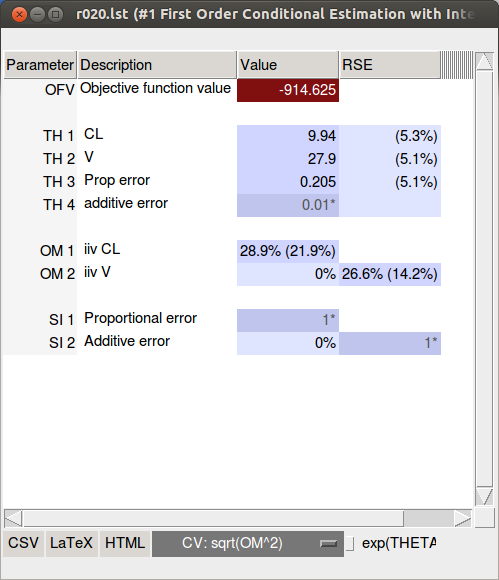
\includegraphics[scale=0.3]{images/estimates_window.png}
    \caption{Parameter estimates window: Single run}
\end{figure}

\begin{figure}[H] \centering
    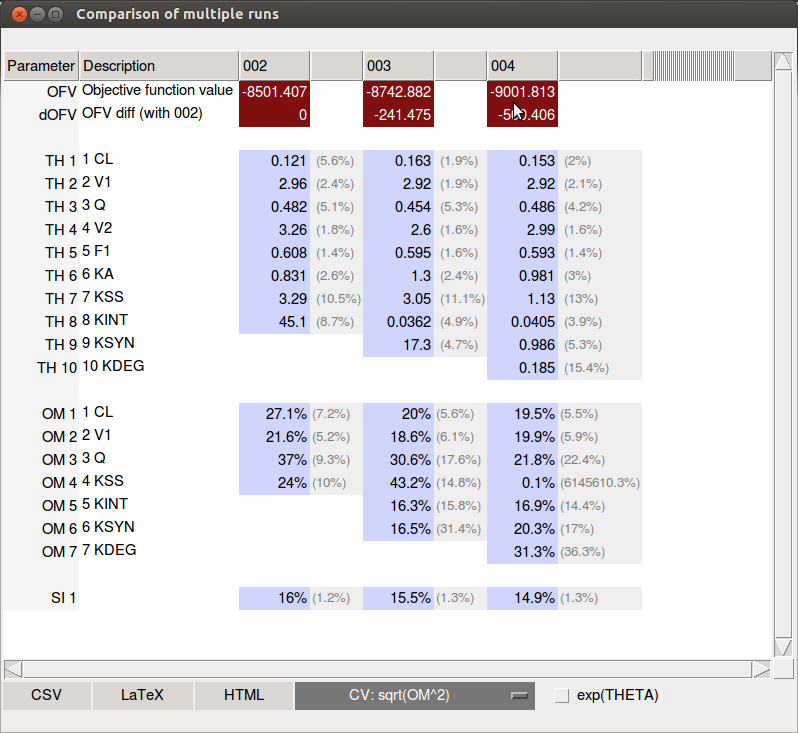
\includegraphics[scale=0.3]{images/compare_estimates.png}
    \caption{Parameter estimates window: Comparing multiple runs}
\end{figure}


\subsection{Run Reports} Run reports with model and run info, and parameter estimates can automatically be generated, and outputted as HTML, \LaTeX \hspace{2pt},
Word, or plain text format. The reports optionally displays basic run
information, run statistics, description and notes, and parameter
estimations, split by implemented estimation methods. The information to
be included in the report can be specified in the menu under `Settings
$\rightarrow$ Run reports'. \LaTeX \hspace{2pt} output is opened in
the specified code editor, but also can be converted automatically to
PDF using pdflatex (if installed).\\

\noindent After a run report is generated it will show up in the list
on the right, under the tab \textit{Reports}. In this tab, also
goodness of fit plots are shown, generated either using the Xpose GUI
in Pirana, or the R scripts library. Double-clicking on any of the
plots or reports will re-open them.\\

\vspace{10pt}
\noindent\scriptsize{\textcolor{Blue}{Note:} \textcolor{Grey} {In the
    run reports, Pirana calculates the RSE for population parameters
    as $RSE_{\theta_i} = \frac{SD_{cov,\theta}}{\theta_{i}}$, but doesn't take into account
    log-transformation of parameters (e.g. when MU-modeling). For
    inter-individual and residual variance ($\Omega$ and $\Sigma$),
    RSE's are calculated as e.g. $RSE_{\omega_{i,i}^2} =
    \frac{SD_{cov,\omega_{i,i}^2}}{\omega_{i,i}^2}$. RSE's given for
    $\omega_{i,i}$ and $\sigma_{i,i}$ are calculated as e.g. $RSE_{\omega_{i,i}} =
    \frac{SD_{cov,\omega_{i,i}^2}}{2 \cdot \omega_{i,i}^2}$ } \normalsize
\vspace{10pt}

\subsection{Intermediate results} When running models through any of
the available methods (nmfe / PsN / WFN), the intermediate results
(parameter estimates, objective function value, gradients) can be
viewed by clicking on the \textit{hourglass}-icon or from
\textit{Tools $\rightarrow$ Intermediate results}. This will open a
window which shows the models that are currently running. By clicking
on a run in the list, Pirana will parse the intermediate files and show the intermediate parameter estimates in the table and the plot. In the plot, you
can choose to show either the gradients (if a gradient method is
used), the intermediate estimates, or the objective function value
(OFV). Make sure that you specify PRINT=1 and MSFO=xxxxx in the
\$ESTIMATION record, to be able to obtain regularly updated
intermediate estimates. From the right-click menu, signals can be
sent to currently running NONMEM processes, such as \textit{stop} and
\textit{next iteration}.

\begin{figure}[H] \centering
    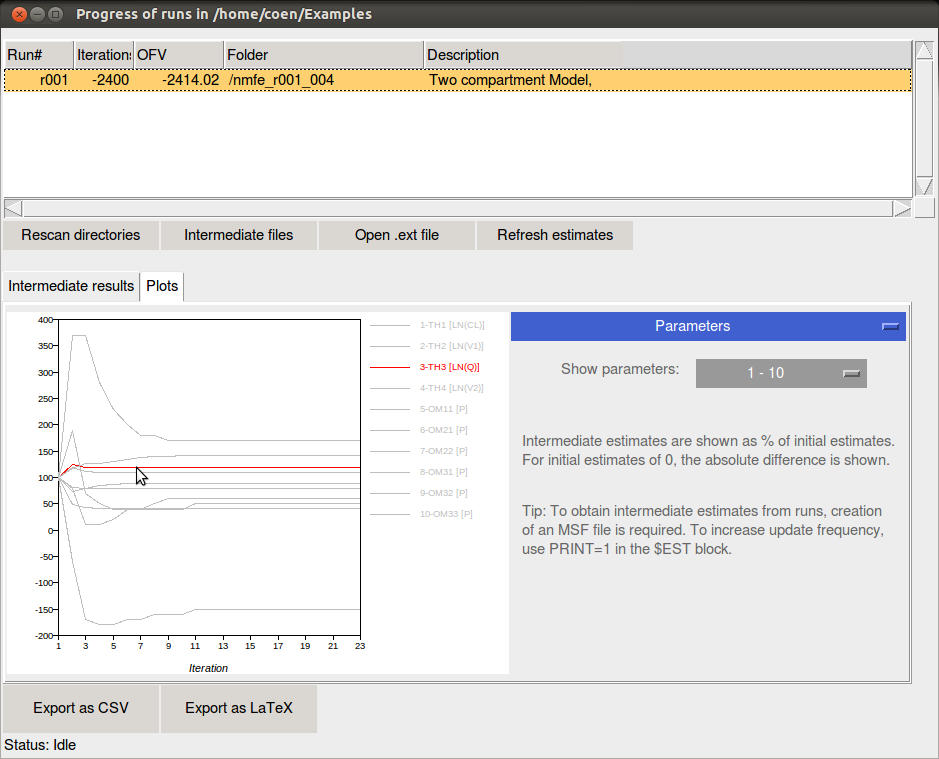
\includegraphics[scale=0.3]{images/intermed.png}
    \caption{Intermediate results}
\end{figure}

\subsection{Run Records}
For all models in the current folder, or a selection thereof, a CSV
run record can be compiled by Pirana that includes all
model and run characteristics, such as model description, estimation
method, objective function value, termination result, etc. An abridged
version of the run record can also be created as a plain text or Word
document.

\subsubsection*{Visual Run Record}
Pharmacometric model development most often progresses in a
hierarchical fashion, using the likelihood ratio test to assess
significance of improved fit between nested models. An appropriate
visualization of the model hierarchy will help the modeler gain better
understanding of key stages in model building, and willl aid in
communicating the model development history to others. Such a
visualization can be generated by Pirana, an example of which is shown below.

\begin{figure}[H] \centering
    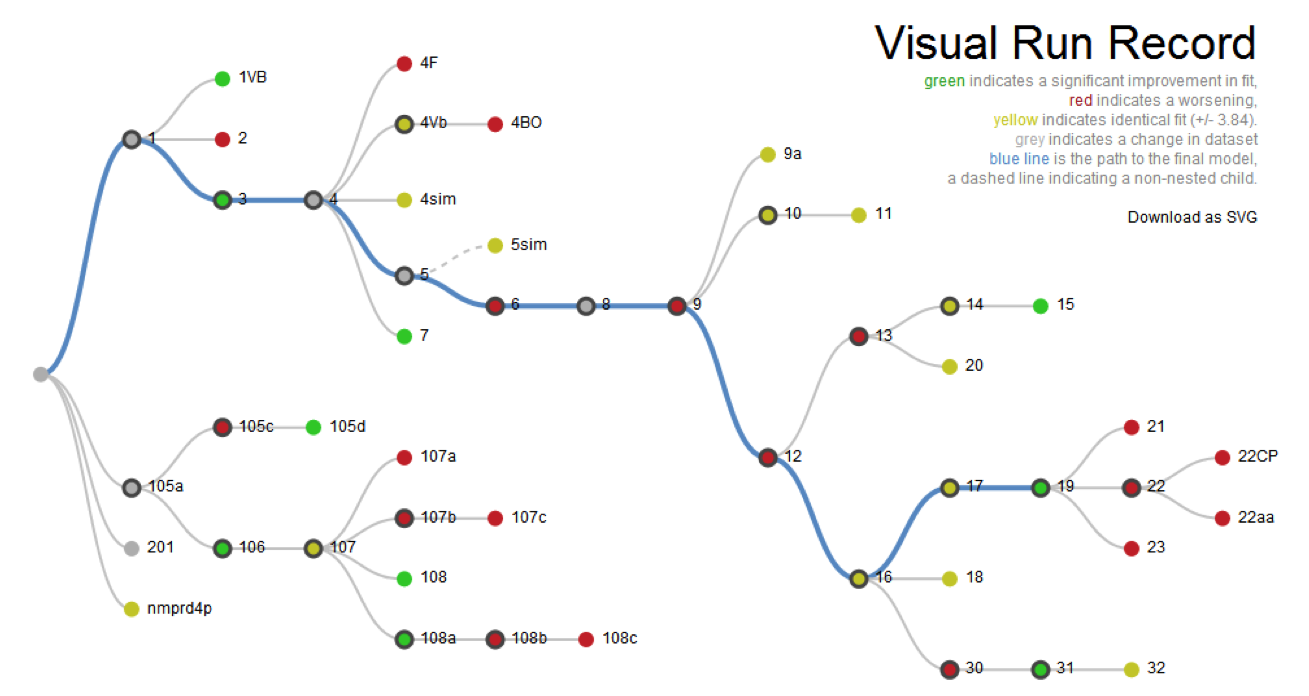
\includegraphics[scale=0.47]{images/vrr.png}
    \caption{Visual Run Record}
\end{figure}

\noindent To create the VRR, Pirana produces Javascript code compatible with the Data-Driven
Documents Javascript library (d3.js). The visualization can be
generated as an SVG image in any modern internet browser. Several
options are implemented that allow customization of the visualization,
and both dynamic and static images can be created. In a VRR, the
hierarchy of models is immediately visible, and using the dynamic
collapsable dendrograms, non-relevant model threads can be hidden from
the visualization. The VRR also shows additional model information
when hovered over the nodes. Colors aid in visualizing the improvement
/ worsening of model fit (green / red), and whether the model has
children or not. In each branch, the nodes are ordered by OFV. When a
final model is specified, the modeling path can be made visible as a
blue line, thereby easily identifying the key runs. The visualization
can be implemented as a horizontal or radial tree, the latter of which
can be used when the model tree is very large.

\subsection{Data Inspector} Pirana is able to construct scatter plots
using the built-in \textit{DataInspector}, e.g. for quickly inspecting
goodness-of-fit, covariate relationships, distribution of etas,
performing data checkout etc. The DataInspector shows all the columns
present in the dataset, which can be mapped to the X- or Y-axis
(shown in figure 3.2). DataInspector can either be invoked by
selecting a model (main overview), or a data file (from the list on
the right). If a model is selected and DataInspector is started,
Pirana will gather the dataset specified in \$INPUT and the table
files created in \$TABLE. It will then ask the user which of these
files to open in DataInspector. If only one file is found, it will
open that one automatically.

\begin{figure}[H] \centering
    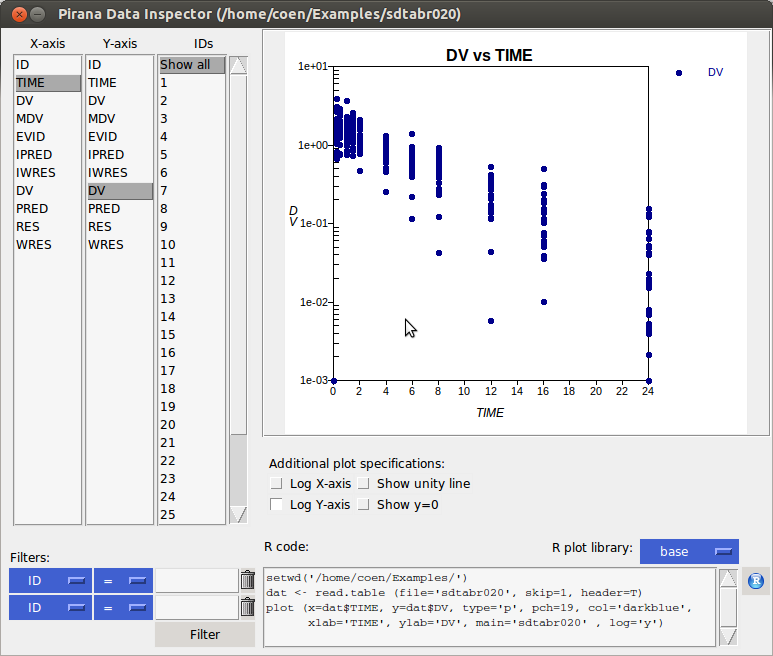
\includegraphics[scale=0.35]{images/plot.png}
    \caption{Pirana DataInspector}
\end{figure}


  \subsection{Visual run records}
The model building process from initial to final model can be visualized using the visual run record.
This can be done via Results  $\rightarrow$ Run records $\rightarrow$ Visual run record.
Here a final model can be selected, and the visual run record will be graphically depicted.

  Pirana can parse NONMEM-generated tables, and CSV-files. Multiple Y values
  can be plotted by holding the Control- or shift-key and selecting
  multiple (up to three) data columns. Inside the plot, regions of
  interest may be selected, which are then zoomed. Double-clicking
  inside the plot region changes back to the previous view. Plots can
  be filtered, which can be useful, e.g. to show only data for one
  patient, or groups of patients or covariates.

  In the text-box below the plot, code is generated that recreates
  the same graph in R, either in \textit{base}, \textit{lattice}, or
  \textit{ggplot2}. This code can be used as a starting
  point for the generation of plots for manuscripts or
  reports. Clicking the `R'-button will invoke the R-GUI or code
  editor.

\subsection{R scripting for creating graphs and file processing}
Pirana includes functionality to run custom R-scripts on output from
models-executions such as NONMEM tables. Scripts can be written by the
user, but a considerable collection of scripts is also bundled with
Pirana, which can serve as starting point for your own
implementations. Scripts are located in three locations, one for
group-wide scripts (in the scripts-folder in the location where Pirana
is installed), one for user-scripts (`home/user/.pirana/scripts'
on Linux, `C:$\backslash$Documents and
Settings$\backslash$user$\backslash$Application
data$\backslash$.pirana$\backslash$Scripts' on Windows), and one for project-specific scripts, stored in the subfolder pirana\_scripts in the current folder. The folder
structure underlying the scripts folders is reconstructed within the
scripts menu, and scripts can be edited either by editing them from
outside Pirana, or by choosing them from the `Edit' menu option.

Scripts can be started by selecting a model, and selecting the desired
script from the scripts menu located in tight tab panel. Pirana invokes R and runs the script in the
directory `pirana\_temp' underlying the active folder.  However,
before execution, Pirana replaces \textit{\#PIRANA\_IN} with an R
list-object which specifies model and results information, e.g. as:

\begin{lstlisting}
models <- list (
   "003" = list (
     "modelfile"       = "003.mod",
     "description"     = "PK model digoxin",
     "reference_model" = "002",
     "data_file"       = "nm_pk_001.csv",
     "output_file"     = "003.lst",
     "tables"          = c("003.TAB", "sdtab003")
   )
 )
\end{lstlisting}

\vspace{15pt} \noindent To automatically load PDFs or images that are created by
R after execution of the script, you should include e.g. the following line in
the script:

\begin{lstlisting}
#PIRANA model_output.pdf
\end{lstlisting}

\noindent where model\_output.pdf is the file that you want Pirana
to load. This may either be a PDF, or a common image format such as
PNG, JPG, or GIF. Please have a look at the scripts included with
Pirana for examples this
functionality.

\subsubsection*{Interactive scripts}
From Pirana 2.6.0 onwards, Pirana has the ability to create
\textit{interactive scripts}, meaning that upon execution of an
R-script, the user will be presented with an
interface that shows plotting and input options. The plotting options can be
specified in the R-script like e.g.:

\begin{lstlisting}
### <arguments>
###       <title label="Plot title">DV vs PRED</title>
###       <x_var label="X-variable">DV</x_var>
###       <xlab label="x-axis label">Dependent variable</xlab>
###       <y_var label="y-variable">PRED</y_var>
###       <ylab label="y-axis label">Pred. concentration</ylab>
###       <subset label="Subset string"></subset>
###       <split_id label="by ID" type="bool">FALSE</split_id>
### </arguments>
\end{lstlisting}

\vspace{4pt}

\noindent This will result in the following interface:

\begin{figure}[H] \centering
    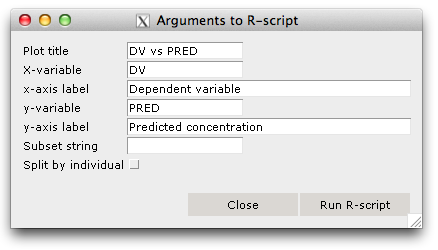
\includegraphics[scale=0.5]{images/interactive_scripts.png}
    \caption{Interactive scripts}
\end{figure}

\noindent In the R-script, the specified options are then available
as the list \textit{arg}, e.g using:

\begin{lstlisting}
ggplot (data=tab, aes (x=get(arg$x_var), 
                       y=get(arg$y_var))) + geom_point()
\end{lstlisting}


\subsection{Xpose support}
After selecting a model, Xpose can be invoked from the scripts menu either by
selecting the integrated Xpose GUI or the calling the (external) Xpose R-menu.
The integrated Xpose GUI allows for execution of Xpose commands. The user can also add
optional arguments to Xpose commands.  Plots can be saved as PDF or
PNG files, or Sweave/knitr code can be generated.

\begin{figure}[H] \centering
    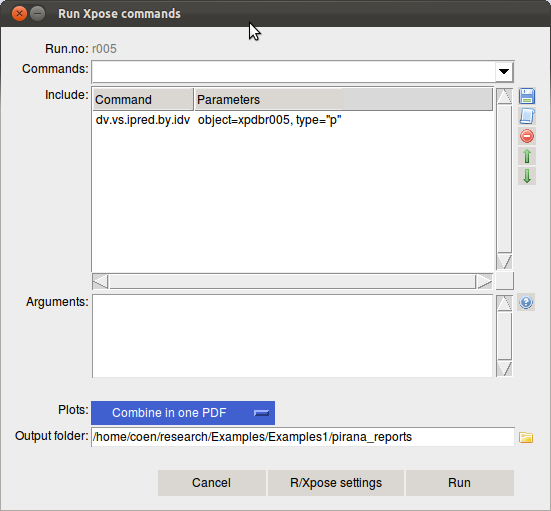
\includegraphics[scale=0.5]{images/xposewindow.png}
    \caption{Xpose window}
\end{figure}

\noindent Besides the commands available in the list, you can also input your
own commands or statements to the list. Lists can be saved for easy
access later on. The general plotting arguments for PDF and PNG
(e.g. {\ttfamily width=10, height=8} can be set in the settings menu
under \textit{R/Xpose})

\subsection{Wizards}
As mentioned earlier, Pirana comes with several wizards, such as a
wizard to create a NONMEM model file, PsN-scm configuration files, and
parallelization files. You can alter these Wizards to your liking, as they are
implemented from wizard-specification files located in
\textit{/wizards} in the Pirana installation folder. Of course, it
is possible to create your own Wizards as well. Just create a
\textit{.pwiz} file in the wizards-folder and follow the instructions
in the template that is provided there. Wizards that are included with
the current version of Pirana are described below:

\subsubsection*{PK model}
This wizard allows stepwise construction of a range of PK models in
NONMEM. It includes all ADVANs in NONMEM, all estimation methods, and
the most commonly used residual error models. Of course, keep in mind
that you have to change the initial estimates and the \$DATA and
\$INPUT records to suit your PK problem.

\subsubsection*{NM parallelization file}
NONMEM 7.2 and higher allow parallization of single runs, which
requires a so-called `parafile', a configuration file for the
parallelization. These files can be created using this wizard.

\subsubsection*{SCM configuration file (PsN)}
The scm command in PsN requires a configuration file. With this wizard
you can create such a file, which includes the most commonly used
options. Please note that more features are available in the scm tool
than are offered as option in the Wizard, so it is advised to acquaint
yourself with the full scm documentation.

\subsubsection*{Dataset template}
This wizard can be used to create an R script that, in turn, generates
a NONMEM simulation data file with specified number of individuals,
doses, observations, dosing times, and covariates. This can be useful
e.g. for quickly setting up simulations in NONMEM.

%%%%
\section{Model translation}
Pirana can translate NM-TRAN models written in any ADVAN routine to
ordinary differential equations (ODEs). The model can be exported to
ADVAN6 (NM-TRAN), to R (using the deSolve library), Berkeley Madonna,
MATLAB and PopED. Also several translators are included that
translate specific parts of NONMEM code to alternate NONMEM code.

\subsubsection*{Translation to other tools}
For R, a multidose simulation is automatically implemented, for the
other converters only single dose simulation is implemented. Pirana
currently does not read in the dataset to extract dosing information.

Pirana extracts the parameter estimates for the structural model
($\theta$), and also the between subject variability matrix
($\Omega$). The latter is however done only when simulating in R or Berkeley Madonna (not available for Matlab at current).
No residual error model is currently implemented in any of the translators, but this can easily be added by the user. 

Porting the model structure to PopED allows evaluation of optimal
study designs (OD). Pirana creates the necessary files for PopED execution, however
the user still needs to provider the details of the design and other optimization settings.

\subsubsection*{MU-model conversion}
Pirana can convert standard NONMEM models to MU-model coding. At
current, Pirana can only convert models written using normal- or
log-normal $\eta$s, e.g.

\begin{lstlisting}
CL = THETA(1) * EXP(ETA(1))
\end{lstlisting}

will be converted into:

\begin{lstlisting}
MU_1 = LOG(THETA(1))  ; ** MU-referenced by Pirana
CL = EXP(MU_1+ETA(1)) 
; Original equation: CL = THETA(1) * EXP(ETA(1))
\end{lstlisting}

\subsubsection*{Difference equations}
For some models written in ODEs, writing some parts of the model in
difference equations can considerably reduce computational burden, while
maintaining parameter precision.\footnote{Petersson KJ et al. J
  Pharmacokinet Pharmacodyn. 2010 Oct;37(5):493-506.} Pirana can help
in setting this up: it will transport all code written in \$DES other
than the $\frac{dA}{dt}$ system to \$PK, and adds some required
code (using \textit{MTIME}).

\section{Batch operations}

Pirana offers functionality to perform batch operations on a set of
models, such as search and replace functions.

\begin{description}
	\item{\textcolor{Grey}{Search and replace in models}} Replaces
          a given search text with another string or block of text in
          the selected models.
	\item{\textcolor{Grey}{Replace block}} This function enables
          you to replace a whole block of code in selected model
          files, e.g. the \$DATA block if you want all model files to
          use a different data file, or the \$THETA block if you want
          to use other initial estimates.
	\item{\textcolor{Grey}{Add code to models}} With this
          function, lines of code can be added to the beginning or the
          end of selected models.
	\item{\textcolor{Grey}{Add code to blocks}} With this
          function, lines of code can be added to a specific block in
          the selected models.
	\item{\textcolor{Grey}{Batch duplicate}} Creates multiple
          duplicates of one model file, with (optionally) updated
          run/table numbers and final parameter estimates.
	\item{\textcolor{Grey}{Random simulation seeds}} In all
          selected models, the \$SIMULATION block will be updated with
          new seeds.
\end{description}

\section{Miscellaneous  functionality}

\subsubsection*{NONMEM help files}
Modeling with NONMEM, and construction of NM-TRAN syntax can be
troublesome at times, and therefore it is convenient to have NONMEM's
help files at your fingertips. Pirana provides a user interface to
these help files, allowing you to filter on keyword. Before help file
interface can be used, the NONMEM help files need to be imported as
the files are not supplied with Pirana. For this, go to `Tools'
$\rightarrow$ `NONMEM' $\rightarrow$ `Import / update NONMEM help
files' to perform this. You can import the information from a local
NONMEM installation or from an installation located on a cluster (over
SSH). After succesful import, the NONMEM help interface is availabe
from the `Help' menu.

\subsubsection*{Code differences between models}
Pirana provides a tool to show code differences, similar to the
\textit{diff} functionality on Unix systems. If one model is selected
and the diff tool is activated (Right-click menu $\rightarrow$
`Model' $\rightarrow$ `Code difference between models'), Pirana will
show the difference between that model and the reference mode (if
specified). If two models are selected, Pirana will show the code
differences between these two models.

\begin{figure}[H] \centering
    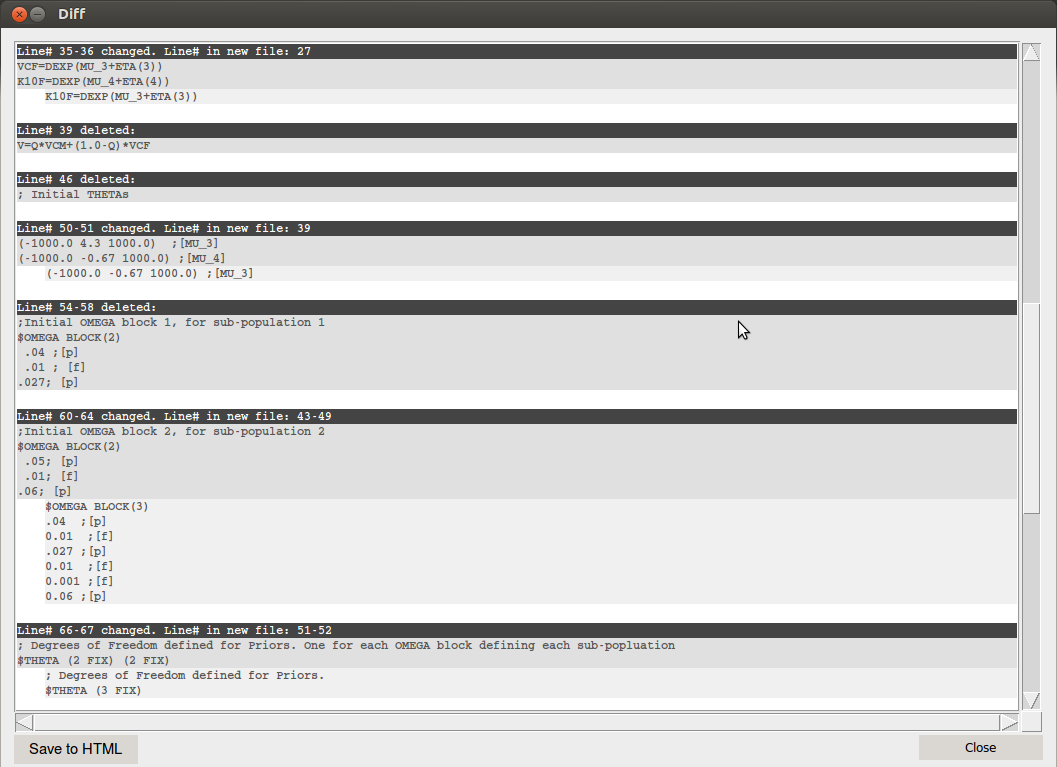
\includegraphics[scale=0.28]{images/diff.png}
    \caption{Code difference between models}
\end{figure}

\subsubsection*{Model Archive: Automatic backup of models and results}
When editing and running models, Pirana can automatically backup all
versions of controlstreams and result files. When this feature is
activated (in the settings menu), intermediate versions of models and
results are saved in a separate folder, every time a model is changed,
or when a new results files is found. The archive can be accessed via
the \textit{Tools} menu, under the option \textit{Model
  Archive}. Details of the run and (if applicable) parameter estimates
can be reviewed. Also, different versions of models can be compared
and restored. The internal Pirana database files (\textit{pirana.dir})
are also backup up, if it has been more than a week since the previous
backup.

\begin{figure}[H] \centering
    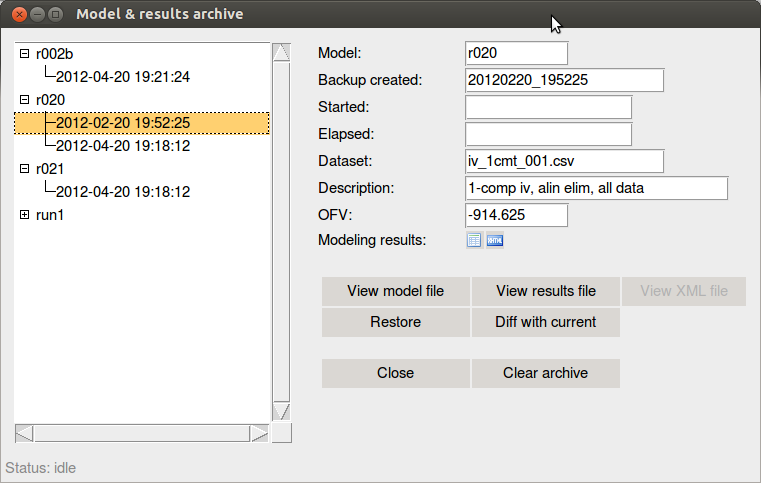
\includegraphics[scale=0.35]{images/modelbackup.png}
    \caption{Model backup / archiving window}
\end{figure}

\subsubsection*{Matrices}
Pirana can automatically extract the covariance, correlation and
inverse covariance matrices from a NONMEM 7+ run (cor/cov/coi files),
and show them in a spreadsheet-like window. These can then also be
automatically exported to an R object, for instance for simulation
purposes.

\begin{figure}[H] \centering
    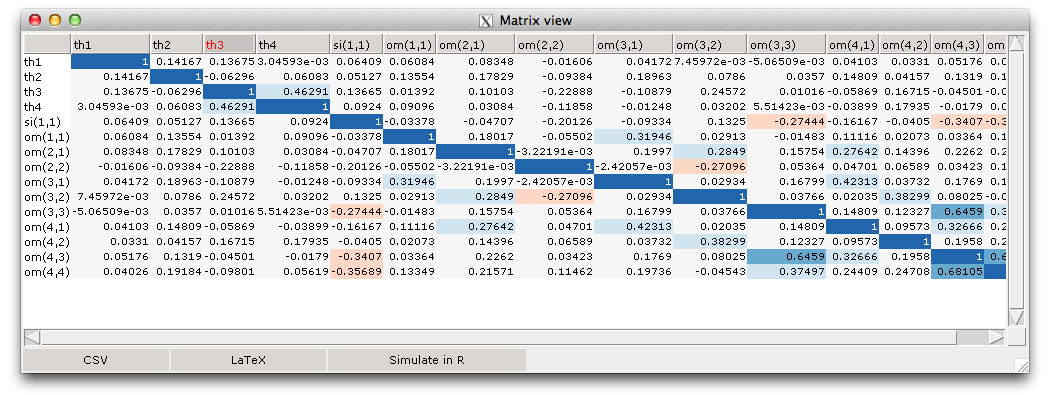
\includegraphics[scale=0.28]{images/cor.png}
    \caption{Correlation matrix}
\end{figure}

\subsubsection*{Miscellaneous tools}

\begin {description}
  \item{\textcolor{Grey}{Correlation calculator}} This opens the
built-in `Correlation Calculator', which can be used to re-calculate a
covariance to a correlation on the SD-scale. The formula for
correlation that is used is:

\vspace{10pt}
$ \rho_{i,j} = \frac{{\omega_{i,j}}^2 }{\omega_{i,i} \cdot \omega_{j,j} }
$
\vspace{10pt}

with $\rho$ specifying the correlation between two elements (i,j) in a
matrix, and $\omega$ specifying elements of $\Omega$ or $\Sigma$.

  \item{\textcolor{Grey}{Checkout dataset}} This will create (and open)
an HTML-file which displays a selected dataset using separate colors for
different event-types. This will thus show the dataset in a slightly more
convenient format for manual inspection than in a spreadsheet. The
function needs at least the ID, TIME and EVID columns in the dataset to work properly.

  \item{\textcolor{Grey}{Calculation of AIC/BIC}} Pirana can calculate
    the Akaike Information Criterion and the Bayesian Information
    Criterion. These criterions are defined as follows:

\begin{equation}
AIC = 2 \cdot k - 2 \cdot ln(L)
\end{equation}

\begin{equation}
BIC = -2 \cdot ln(L) + k \cdot ln(n)
\end{equation}

with $k$ the number of parameters in the model, $L$ the maximized
value of the likelihood function, and $n$ the number of observations
in the dataset used in fitting the model. The calculation of these
criterions is however not so straightforward for non-linear mixed-effects
models, and the weights/penalties applied to parts of the equation can
be different in different circumstances. Pirana allows the penalties
to be changed when it calculates the AIC/BIC. From the right-click
menu, select \textit{Model actions} $\rightarrow$ \textit{Calculate
  AIC/BIC}, and a dialog window will open which will present the
options available. Some useful literature is listed below.

\scriptsize
\begin{itemize}
\item Vaida and Blanchard, Conditional Akaike information for
mixed-effects models. Biometrika, 2005. 92(2): p. 351-370.
\item Liang, et al., A note on conditional aic for linear
mixed-effects models. Biometrika, 2008. 95(3): p. 773-778.
\item Hodges and Sargent, Counting degrees of freedom in hierarchical
  and other richly�]parameterised models. Biometrika (2001) 88 (2): 367-379.
\item Donohue et al., Conditional Akaike information under generalized
  linear and proportional hazards mixed models, Biometrika (2011) 98
  (3): 685-700.
\item Delattre et al., BIC selection procedures in mixed effcts
  models \\ http://hal.inria.fr/docs/00/69/64/35/PDF/RR-7948.pdf
\end{itemize}
\normalsize

\item{\textcolor{Grey}{Clean-up folder}} This tool can be used to
  clean-up files that NONMEM generates when running a model (e.g
  INTER, FSTREAM, etc.). So if you run a model in the main model
  folder (which is not considered good modeling practice),
  you can use this tool to clean up after model execution.

\end{description}

\clearpage
\section{Conventions and Methods}
\subsubsection{Model file conventions}

\begin{itemize}
\item Users of PsN and Xpose likely follow the `Uppsala convention' of
  having model files named like \textit{run1.mod}, \textit{run2.mod},
  etc. This is recommended for Pirana users as well, although
  Pirana is flexible in this respect. Note that Pirana removes
  the 'run' from the modelfile name in the model overview.
\item Pirana looks for a description of the model in the first part of
  the model file. It adheres to PsN's run record standards.
  If the PsN run record is not used,
  Pirana searches for the words `\ttfamily{\$PROBLEM}' \normalfont or
  `\ttfamily{Model desc:}' \normalfont to extract the model
  description.
\item If you want to use the hierarchy functionality for models, you
  should specify the reference model in the first few lines of the
  model file. Again, best is to use PsN's run record specification, but
  Pirana is flexible and also compatible with Census, and
  understands the following syntaxes:

\begin{lstlisting}
;; 1. Based on: 001.mod
; Ref. model:001.mod
; Ref:001.mod
; Parent=001.mod
\end{lstlisting}

\item Model parameter descriptions need to be specified
after a semi-colon, e.g.

\begin{lstlisting}
$THETA
(3, 5, 11) ; CL/F
(10, 50, 100) ; V/F
\end{lstlisting}

Note that Pirana reads these decriptions from the model file (and
not from the output file). To be read correctly, covariance block need
to be specified as:

\begin{lstlisting}
$OMEGA BLOCK(2)
0.1 ; IIV CL/F
0.05 ; COV CL~V
0.1 ; IIV V/F
\end{lstlisting}

or as:

\begin{lstlisting}
$OMEGA BLOCK(3)
0.1           ; IIV CL/F
0.05 0.1      ; IIV V/F
0.01 0.05 0.1 ; IIV KA
\end{lstlisting}

\item When models are to be executed in a separate directory, files
  needed for compilation (e.g. additional Fortran routines in .FOR
  files), are copied automatically by Pirana. These files should be
  specified in the \ttfamily{OTHER} \normalfont and \ttfamily{CONTR}
  \normalfont entries on the \ttfamily{\$DATA} \normalfont record. If
  more additional files are needed, you can instruct Pirana to copy
  these by adding this line to your control stream:

\begin{lstlisting}
; INCLUDE=file1_to_be_copied.ext,file2_to_be_copied.ext,etc
\end{lstlisting}

Note that PsN has it's own functionality for doing this.

\end{itemize}

\section{Keyboard shortcuts}
The following keyboard shortcurts are available in Pirana:
\begin{itemize}[noitemsep,topsep=5pt,parsep=1pt,partopsep=0pt]
  \item        Ctrl-R: Run model
  \item        Ctrl-L: Open NM output file (.lst)
  \item        Ctrl-N: New model file
  \item        Ctrl-D: Duplicate model file
  \item        Ctrl-P: Show parameter estimates for run(s)
  \item        Ctrl-T: HTML-file from NM output
  \item        Ctrl-E: Execute model (PsN)
  \item        Ctrl-B: Bootstrap model (PsN)
  \item        Ctrl-V: VPC from folder (PsN)
  \item        Ctrl-U: Update inits (PsN)
  \item        Ctrl-X: Run Xpose commands
  \item        Ctrl-A: Select all models
  \item        Ctrl-+/-: Increase / decrease font size
  \item        Ctrl-, : Open settings window
  \item        F5 : Refresh current folder
\end{itemize}

\clearpage
\section{Command line parameters}

\begin{itemize}[noitemsep,topsep=5pt,parsep=1pt,partopsep=0pt]
  \item   \begin{verbatim}-portable\end{verbatim} Use Pirana in portable mode, e.g. from a USB-stick, leave no footprint on computer.
  \item   \begin{verbatim}-console\end{verbatim} Leave console window
    open. This may be useful when Pirana hangs or crashes, as
    sometimes an error may be shown on the command line. (Fortunately
    Pirana hardly ever crashes, though).
  \item \begin{verbatim}-debug\end{verbatim} Print information during
    startup. This may be useful when for some reason Pirana doesn't
    start up, possibly due to some missing file or incomplete
    installation.
  \item \begin{verbatim}-time\end{verbatim} Print some information during
    folder reading. Useful for troubleshooting on slow network connections.
\end{itemize}

\newpage

\section{Troubleshooting / FAQ}

Below are some answers to commonly asked questions. Note that a more
elaborate and up-to-date FAQ is also available on the website.

\begin{itemize}

\item \textit{Why the name Pirana?}

  \vspace{5pt} An acronym for: Pirana is a Resourceful Assistant in NONMEM Analysis.

\item {I'm running on Windows, but for some reason Pirana won't start (anymore)}

\vspace{5pt} Please check for any errors during startup by using the {\tt -console -debug} arguments on the command line. If there is any problem during initialization of Pirana, you can try to reset the default settings in Pirana by running {\tt pirana.exe -refresh} in the console (this works only in version 2.5.1 or later. For earlier versions, remove the folder {\tt \%HOME\%/.pirana} manually, where \%HOME\% is your home folder). This will remove your current settings and re-install the defaults. Then, try to restart Pirana in the regular way. If this doesn't work, please report it as a bug with a screendump of the console output.

\item \textit{ In Pirana's model overview table, I see some models but
    no results...?}

  \vspace{5pt} First check if you have the extensions set correctly in
  preferences, e.g. .mod/.lst for model/results files. If this doesn't
  solve the problem, it may be due to the fact that your database file
  for that folder is corrupt. In the current folder, try renaming
  pirana.dir to pirana.dir.bak and refresh the folder. This error may
  sometimes occur when you have been using an old version of Pirana
  previously ($<$2.1.0). On Linux, problems have been reported with
  old versions of the Perl modules DBI and DBD::SQLite. Make
  sure you have versions 1.6 or higher or 1.14 or higher, of these
  respective modules. (You can check this by typing the following on
  the command line:

  \begin{lstlisting}
  perl -MDBI -e 'print "$DBI::VERSION"'
  perl -MDBD::SQLite -e 'print "$DBD::SQLite::VERSION"'
  \end{lstlisting}

\item \textit{On startup of Pirana on Windows, it complains that it
    can't find the file libgcc\_s\_dw2/1.dll, libstdc++-6.dll, or perl516.dll.}
  Pirana needs these library files to function, and therefore we
  supply them with Pirana (in the folder where you installed it,
  probably C:$\backslash$Program Files$\backslash$Pirana). On some
  systems however, it needs to be copied to the folder
  "C:$\backslash$Windows" or
  "C:$\backslash$Windows$\backslash$system32" for Pirana to
  function.

\item \textit{I can't seem to start any NONMEM runs or use PsN. Basically, noothing happens, and no error message is produced.}

 \vspace{5pt} \textbf{On Windows:} The likely cause of this error is that Pirana can't start
your command shell. Please check in your "Environment variables" in
the Control panel, that 

\begin{lstlisting}
C:\Windows\system32
\end{lstlisting} 

is included in the PATH
environment variable. If not, add it. While you're at it, check also
that the variable ComSpec is set to: 

\begin{lstlisting}
C:\Windows\system32\cmd.exe
\end{lstlisting}

 \vspace{5pt} \textbf{on Mac OSX:} This is most likely because Pirana is not able to find X-terminal. Please update your settings in Pirana, in Settings 
 $\rightarrow$ `Miscellaneous'  $\rightarrow$ `Terminal to start NONMEM runs in'. Change `xterm' into `/usr/X11/bin/xterm', and it should work fine.

\item \textit{When I open a csv file in Excel from Pirana (and in
    general), I get the error message that the file is recognized as a
    SLYK-type file, and
    therefore cannot open the file.}

  \vspace{5pt}
  This is due to the fact that the first column in your dataset is
  named "ID". Renaming the column (e.g. 'id') or inserting a column
  before it will solve the problem. When converting and opening table
  files, the "ID" column is automatically converted to "id" by Pirana
  to avoid these issues.

 \item \textit{Running on Mac OS X, after starting Pirana, nothing seems to happen.}

 \vspace{5pt}
 Make sure you have Xcode, the Xcode command line tools, and XQuartz installed. Update to the latests OS X version. 

 \item \textit{Where does Pirana store the notes I make in the model overview?}

\vspace{5pt} Pirana stores your notes in a database-file ({\tt pirana.dir}) in the current folder. So, if you would install a new version of Pirana, or move your model folder to another place, your notes will not be lost. The database file contains also some other information about the run results (OFV, run success, etc.) and can of course be read out manually as well, using {\tt sqlite3}.

\item \textit{I'd like to cite Pirana in a report or article.}

\vspace{5pt} Please cite Pirana as: Keizer RJ et al.; Comput Methods Programs Biomed 2011 Jan;101(1):72-9; Pira\~na and PCluster: a modeling environment and cluster infrastructure for NONMEM. PubMed

\end{itemize}

%%% Monolix

\clearpage
\section{Monolix}
Since version 2.7.0b, Pirana includes support for Monolix, the SAEM nonlinear mixed-effects modeling
system developed by Lixoft. Pirana supports both the stand-alone version and the Matlab version of Monolix,
and interacts with Monolix both on Windows and on Linux. Pirana requires that models are 
written in MLX-TRAN, the modeling language derived from NM-TRAN that can be used to write models in 
Monolix. Similar to NONMEM models, MLX-TRAN models are shown in the main overview automatically when
a folder is loaded in Pirana. Pirana will automatically switch to \textit{Monolix mode} when it detects
MLX-TRAN models in the folder (the extension of which can be set under \textit{Settings}). MLX-TRAN can be run from the Monolix submenu, 
and results and parameter estimates can be viewed in a similar fashion as the results obtained from NONMEM.

\vspace{10pt}
\noindent\scriptsize \textcolor{Blue}{Note:} \textcolor{Grey} {
The Monolix functionality in Pirana is still in development, and not all features available for NONMEM are available for Monolix. Also, a more detailed description of available features will be added to a future version of this manual. 
If you are interested to have Monolix-specific features implemented in Pirana, please let us know.}
\normalsize

%%% CLUSTERS %%%%%%%%%%%%%%%%%%%%%%%%%%%%%%%%%%%%%%%%%%%%%%%%
\chapter{Pirana and clusters}

\section{Clusters} Pirana supports interaction with Linux-based
clusters on which NONMEM and/or PsN are installed. The Job-schedulers
Sun Grid Engine (SGE), Torque and Condor are supported. In addition,
SSI-type cluster managers such as MOSIX should also work without
problems. Connecting to a cluster is established using the SSH
protocol, or any method that can be invoked from the command line. Two
methods are available for using Pirana with a grid/cluster system,
which involve installation of Pirana either on the local system or
directly on the cluster server. The following paragraphs discuss these
two separate methods.

\vspace{10pt}
\noindent\scriptsize \textcolor{Blue}{Note:} \textcolor{Grey} {Single-system image clusters such as MOSIX, openMOSIX and
Kerrighed distribute processes automatically accross nodes, and therefore no alternative setup is required in Pirana.}
\normalsize

\subsection{Method 1: Server-based installation}
When using this approach, Pirana is only installed on the
cluster-server, not on the local machine. Pirana is executed from the
local machine using X-over-SSH window tunneling. This has the
advantage of requiring only one central installation of Pirana for the
entire modeling group, and Pirana and other modeling software is
installed in a controllable environment. A disadvantage is that the
interface is usually a bit slower. Also all auxiliary software (Office
suite, HTML-browser, R and an R-GUI, etc.) resides on the
cluster. Especially when using this method over larger distances
(i.e. across internet), the performance of Pirana may be impaired due
to the server-client transmission of the full GUI, but this of course
depends on the bandwith of your connection and can be tested easily.\\

\subsubsection*{X-over-SSH tunneling}
On the local machine it is necessary to have an X window system
installed.  For Linux users this is likely already installed. Mac OSX
users need to install the XQuartz system. For Windows, a good X window
manager is Xming, which can be obtained for free from
http://sourceforge.net/projects/xming/. After installation of Xming,
start the Xming X-window server. An alternative to Xming is Cygwin/X.

\subsubsection*{Using the cluster}
If everything is set up correctly, and the X-window server is started,
Pirana on the cluster can be accessed through SSH, e.g. by using the
SSH client. Now, you should be able to see the Pirana main window. If
you get an error saying that the display cannot be started on
localhost, you may have to enable X-window forwarding in OpenSSH or in
PuTTY. When using PuTTY, it is essential to use the PuTTY terminal
directly, and not plink.exe. The latter program tends to make Pirana
crash often, probably due to terminal incompatibility. OpenSSH can
also be used.

\subsection{Method 2: Local installation}
The other method is to install Pirana on the local machine, and
connect to the cluster using Pirana and third-party SSH software. We
usually recommended this installation approach as it offers a more
stable interface (independent of network speed), and does not require
installation of auxiliary software on the cluster. It will however
require a few additional local installations. First, you need to mount
the cluster drive with your data on your local PC (e.g. using sshfs on
Linux/Mac or ExpanDrive on Windows).  This can be set up e.g. using
ExpanDrive to connect to the cluster through SFTP. Alternatively, if,
on the remote cluster a Samba server is installed, a connection can be
established by giving the following command:

\begin{lstlisting}
NET USE Z: \ \server_name\<name> /user:<name> /persistent:yes
\end{lstlisting}

\noindent Both on Windows and Linux, you need to specify in the
preferences the mounted remote diskspace and the local location, which
is used by Pirana to translate local paths to paths on the remote
cluster.

\noindent Secondly, an SSH client  needs to be installed, which is probably
already the case on Linux or Mac. On Windows, we have good experiences
with PuTTY
(http://www.chiark.greenend.org.uk/$\sim$sgtatham/putty/) and OpenSSH (download from
http://sshwindows.sourceforge.net/).

In the \textit{Settings $\rightarrow$ Clusters: SSH} menu, specify the
command you use to connect to the cluster on the command line, e.g.:

\begin{lstlisting}
ssh user@server.domain.ext
\end{lstlisting}

\noindent Note that Pirana needs passwordless SSH-access to the cluster, so make
that you have an RSA key pair installed (explained in the next
section). If you use PuTTY on Windows, you can also choose to supply
the password on the command line instead, e.g.:

\begin{lstlisting}
plink -l username -pw password server.domain.ext
\end{lstlisting}

\noindent although from a security perspective this is not recommended.) 
Models can then be run in a similar fashion as explained in
the section for running models locally, just select the cluster to run
on from the nmfe- or PsN run windows.

\subsubsection*{Installing Public and private authentication keys}

Either on Windows or Linux, type in a shell/console window: (If you use PuTTY instead of OpenSSH, use the Keypair generator program instead.)\\
\begin{lstlisting}
ssh-keygen -t rsa
\end{lstlisting}

\noindent When asked for a passphrase, just press $<$Enter$>$.  Now a
public and a private key have been created in
\begin{verbatim}c:\Documents and Settings\<Name>\.ssh}\end{verbatim} (Windows) or
\begin{verbatim}/home/username/.ssh\end{verbatim}(Linux). In you home
directory on the cluster, if it doesn't exist already, create the
folder `.ssh'. In this folder, create the file `authorized\_keys' (no
extension) and add the contents of id\_rsa.pub to that file and save
it. Now you should be able to login without being asked for a password. 
If SSH asks you if you want to accept the cluster as valid host, accept). Keep your private key
secret. In the Pirana preferences, speficy the username to connect to
the cluster (ssh\_login).

\vspace{10pt}
\noindent\scriptsize \textcolor{Blue}{Tip:} \textcolor{Grey} {if you experience delays (about 5 secs) when logging in to the
    server by SSH, this may be caused by a reverse DNS lookup. You can
    circumvent this by adding `useDNS no' to the file
    /etc/ssh/sshd\_config on the server. Restart the ssh server for
    the changes to take effect: sudo /etc/init.d/ssh restart}
  \normalsize

\section{Interaction with job schedulers}
Pirana has integrated support for Sun Grid Engine (SGE), Torque, and
Condor job scheduling systems.  In the settings menu, clusters and job
schedulers can be configured.  For Torque and Condor, auxilliary
scripts can also be defined in the settings menu.  Jobs submitted
through SGE, Condor or Torque can be monitored and managed using the
integrated job monitor (via View menu or top-right
icon).  If PsN is used, Pirana also indirectly supports the use of
additional job scheduling systems that are supported by PsN (SLURM,
LSF, UD, MOSIX, LSF).  No integrated run managers are currently
available in Pirana for these additional cluster systems.

\subsection{Working with the SGE}
Submitting the execution of a model using nmfe to the SGE, Torque, or Condor can be done
by selecting the `Run on SGE or Torque' from the \textit{nmfe} or \textit{PsN} dialog windows.
This submits the model using \textit{qsub} instead of starting it directly. 

\begin{figure}[hbt] \centering
    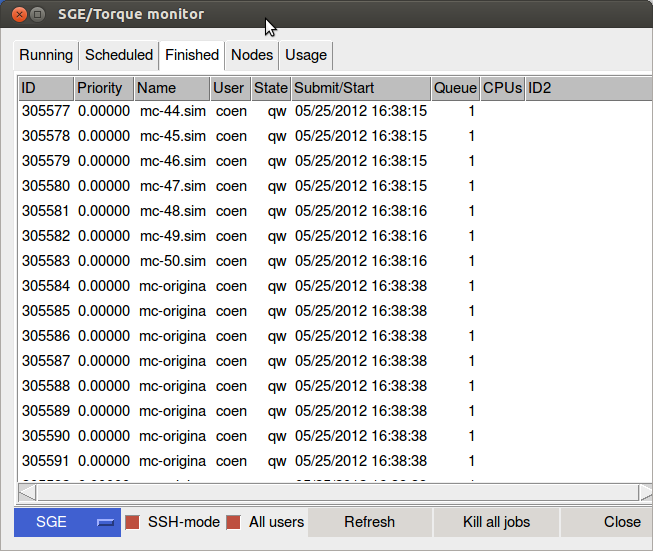
\includegraphics[scale=0.3]{images/Figure3_1_SGEmonitor.png}
    \caption{Job monitor}
\end{figure}

\section{Working with PCluster}
Additionally, Pirana supports the construction of a simple
Windows-based clustering system (PCluster). PCluster allows set up of a cluster using
e.g. PCs of colleagues, and is easy to install on Windows systems.
Please note that this kind of setup is inferior to the clusters
mentioned above in terms of stability and performance. The development of PCluster has now been
discontinued, and no active support will be provided for this
feature. If you still want to try the PCluster, there is a short
manual available upon request.

%%%%%%%%%%%%%%%%%%%%%%%%%%%%%%%%%%%%%%%%%%%%%%%%%%%%%%%%%%%%%%%%%%%%%%%%%%
\chapter{Automated modeling workflow in
Pirana}

\section{Background}\label{background}

An automated workflow alleviates the burden on modeling scientist by
removing the repetitive task of running and evaluating many candidate
models, standardizes the model development between modelers, and
standardize the results reported from such an analysis ultimately
leading to higher quality of PopPK analyses (\emph{Schmidt et al. JPKPD
2014 Aug}). In Pirana (version \textgreater{}= 2.10), such a workflow is
made available, and in this chapter we will walk through an example of
an automated population PK analysis.

\section{Tutorial}

For this chapter, we will use the template model library that is
provided with Pirana, and a (simulated) dataset of an iv-administered
drug also provided with Pirana (\texttt{demo.csv}).

\subsubsection*{Start}

Start Pirana Create a new project folder somewhere on your hard-drive
(or cluster). Browse into this folder (with Pirana). In this folder,
copy the file \texttt{demo.csv} that is included in the Pirana
installation folder (\texttt{Pirana/automod\_library/demo/demo.csv}). In
Pirana, go to \textbf{Tools} --\textgreater{} \textbf{Automated modeling
workflow}.


\subsubsection*{Screen 1: Models and
dataset}

\begin{figure}[htbp]
\centering
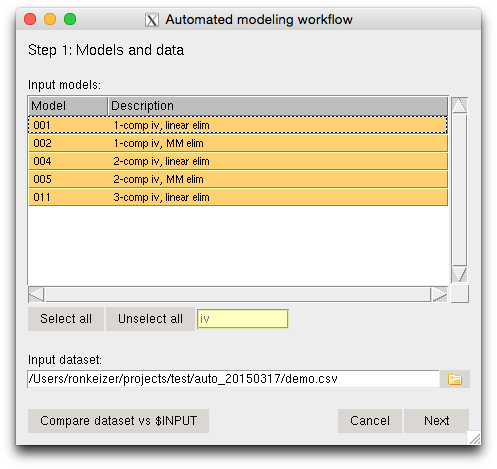
\includegraphics[scale=0.5]{images/screen1.png}
\caption{Screen 1: Models and dataset}
\end{figure}

This screen shows all models available in the library and which can be
selected to be included in the analysis. Use the filter for conveniently
selecting e.g.~only \emph{iv} or only \emph{oral} models. The dataset
should of course be specified as well before you can advance to the next
step. By default, it will use the first \texttt{.csv} file in this
folder (in alphabetic order).

When models and dataset have been selected, you should check whether the
\texttt{\$INPUT} record in the models matches with the headers in the
dataset. For this, click the button \texttt{Compare dataset vs}\$INPUT`.
This will bring up screen shown in figure 2:

\begin{figure}[htbp]
\centering
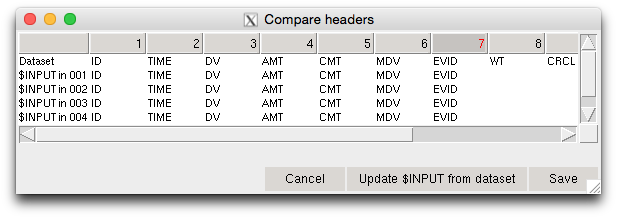
\includegraphics[scale=0.5]{images/compare.png}
\caption{Compare/set input headers}
\end{figure}

If the \texttt{\$INPUT} in the models (shown in rows 2-\ldots{}) does
not match up with the dataset (shown in row 1), you can click the button
\texttt{Update \$INPUT from dataset}. This will create a new \$INPUT
record for all models. After clicking \textbf{Save}, when the models
will be written (in step 3 of the automated analysis), the \$INPUT
records in all models will be changed to the new one. It is left to the
user to make sure that the variables used in the model are still
included in \$INPUT, as there is no extra check in place for that.

For our current analysis, we will select all \emph{iv} models, so filter
on \emph{iv}, and select the remaining models. Update the
\texttt{\$INPUT} records, click \emph{Save} and then \emph{Next} to
advance to the next step.


\subsubsection*{Screen 2: Setting initial parameter
estimates}\label{screen-2-setting-initial-parameter-estimates}

In the second screen, we can set initial parameter estimates, as well as
lower and upper bounds. All parameters are read from the models that
were selected in step 1. The parameter descriptions are defined in the
models as comments to \texttt{\$THETA}, \texttt{\$OMEGA}, and
\texttt{\$SIGMA} blocks, like e.g.

\begin{figure}[htbp]
\centering
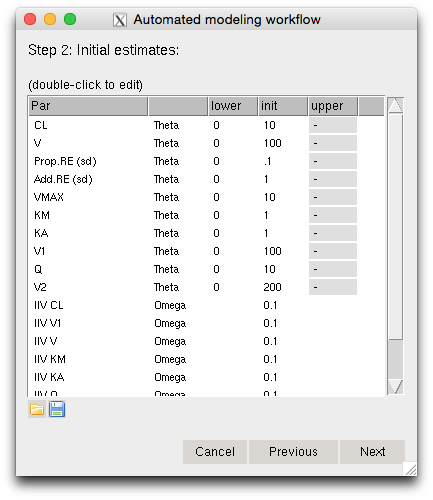
\includegraphics[scale=0.5]{images/screen2.png}
\caption{Screen 2: Initial parameter estimates}
\end{figure}

\begin{verbatim}
$THETA
(0, 5, 100); CL
(0, 5, 100); V

$OMEGA
(0.1); CL
(0.1); V

$SIGMA
0.05 ; proportional error
\end{verbatim}

\emph{Note:} At current, correlations in \$OMEGA and \$SIGMA cannot be
specified for an automated analysis. I.e. only the diagonal elements of
\$OMEGA and \$SIGMA can be specified in the template models if you want
to update them in this step. You can still include models that have full
\$OMEGA or \$SIGMA blocks as template model, however you cannot provide
descriptions (as comments) to the parameters in the block, and you
cannot update them in this step of the analysis.

The two buttons below the parameter grid can be used to save and
(re-)load parameter definitions to file.

For our analysis, let's leave the parameters as they are. Click
\textbf{Next} to advance to the next step.


\subsubsection*{Screen 3: Folders}\label{screen-3-folders}

\begin{figure}[htbp]
\centering
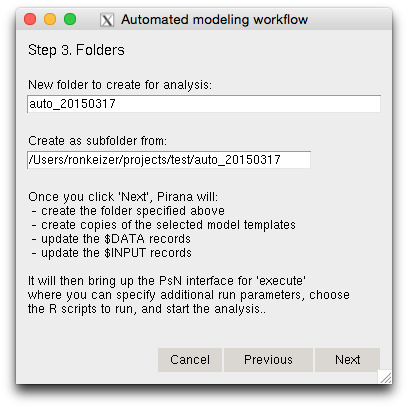
\includegraphics[scale=0.5]{images/screen3.png}
\caption{Screen 3: Folders}
\end{figure}

In this screen we can specify where to create the new models and run the
analysis. By default it will generate a new folder name based on the
current date, and as a subfolder from the current folder in Pirana. This
screen also lists the actions that Pirana will perform once you click
\emph{Next}.

Let's use the defaults and click \emph{Next}.


\subsubsection*{Screen 4: PsN dialog}\label{screen-4-psn-dialog}

\begin{figure}[htbp]
\centering
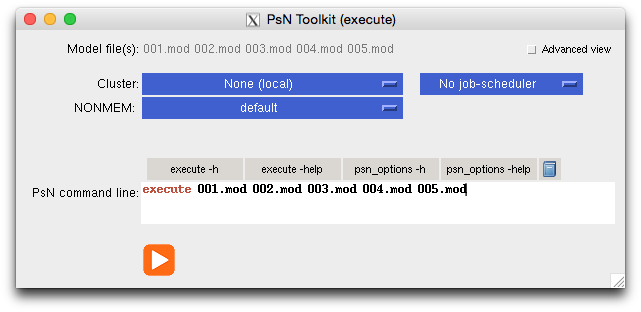
\includegraphics[scale=0.5]{images/psn_simple.png}
\caption{Screen 4: PsN}
\end{figure}

Pirana should now have switched automatically to the new folder where
you will see the newly generated models. Pirana will also automatically
bring up the PsN \texttt{execute} dialog. In this dialog, if you switch
to \textbf{Advanced view}, you can select which R script(s) to run after
all runs have been completed to generate goodness-of-fit plots. Click
the \emph{folder} icons next to the R scripts textboxes to select R
scripts (or batch files) to run after (or before) the analysis (figure
6).

\begin{figure}[htbp]
\centering
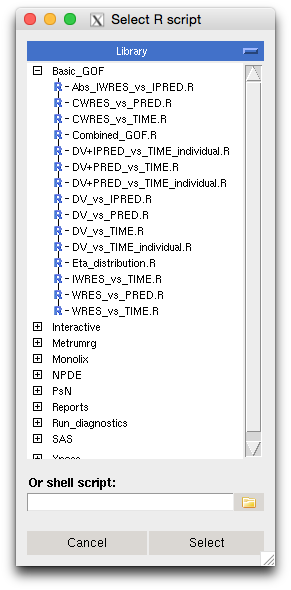
\includegraphics[scale=0.5]{images/run_r.png}
\caption{Select R script}
\end{figure}

For our analysis, we will select the \textbf{Basic GOF plots as single
doc} from the \texttt{Reports} folder to create GOF plots for all
models. The graphical report will automatically be opened, but is also
available from the \emph{Reports} tab on the right.

If you have not selected R scripts to be executed automatically after
the analysis has completed, you can still create them afterwards by
selecting the runs and running any R script from the \textbf{R} tab on
the right side of the Pirana window.

Besides the graphical report, Pirana can generate a \emph{numeric}
report for the analysis, including e.g.~OFVs, basic run information and
parameter estimates. This document is not generated automatically but
has to be requested manually after the analysis is complete: Make sure
Pirana is still in the folder where the analysis was run, and then go to
\textbf{Tools} --\textgreater{} \textbf{Automated modeling workflow}
--\textgreater{} \textbf{Report}. On the first page you will see an
overview of all models included in the analysis and their respective
OFV, AIC and BIC (figure 7). The subsequent pages includes information
on each individual run in the analysis.

\begin{figure}[htbp]
\centering
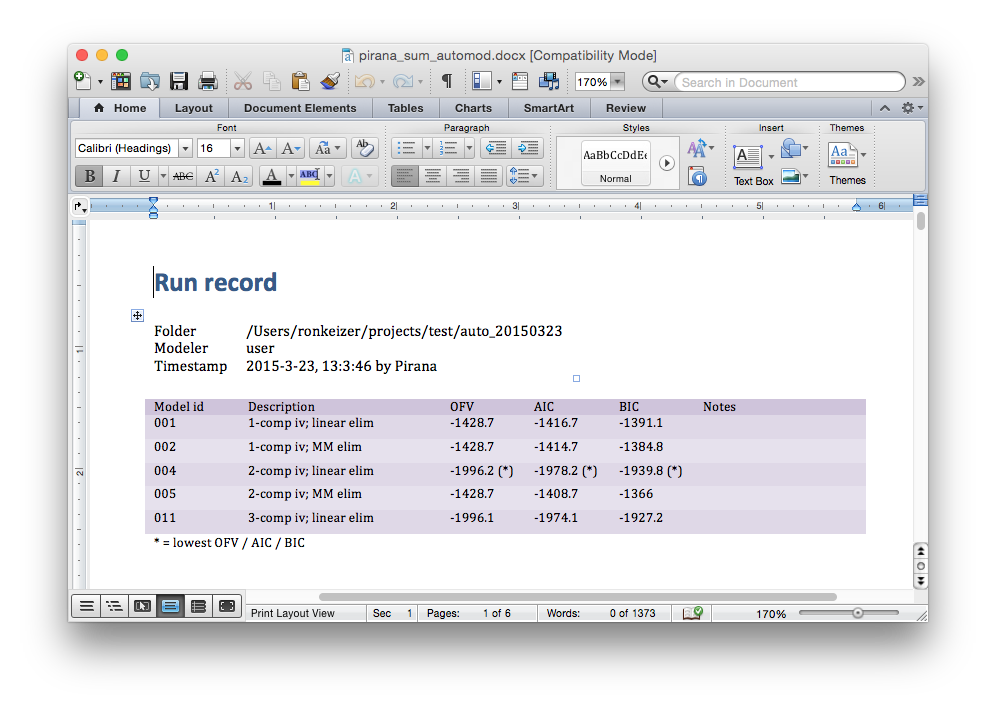
\includegraphics[scale=0.5]{images/report.png}
\caption{Report in Word}
\end{figure}



%%%%%%%%%%%%%%%%%%%%%%%%%%%%%%%%%%%%%%%%%%%%%%%%%%%%%%%%%%%%%%%%%%%%%%%%%%
\chapter{cPirana}
cPirana is a simple, `lite' version of Pirana that runs on the Unix command line. 
There are several reasons that we think cPirana is a useful addition to our primary software product. 
Over the years we have encountered many --usually more experienced--
modelers that prefer to work from the command line. We still think a user interface (be it graphical or
console-based) can greatly increase productivity and make the modeling process
easier in general. For those modelers, we hope cPirana is a welcome addition to their workflow. 

\vspace{10pt}

\noindent Secondly, while working on cluster through a slow internet connection, the interface may become slow. 
Version 2.7.0 included already many speed improvements that improves working on slow connections. However, 
e.g. when traveling, one might be only interested in making a few small code changes and restart a model.
If a computer with Pirana is not available, or if the internet connection is very slow, you probably will still 
be able to login to your cluster over ssh. If cPirana is installed on this cluster, you will have the ability to
use most Pirana functions directly from the command line interface.

\vspace{10pt}

\noindent Finally, already from our earliest versions of Pirana, we intended to extend the implementation
of Pirana to smartphone or tablets, allowing for increased mobility
and connectivity. While the implementation of a true dedicated Pirana
app is currently beyond the capacity of our small development team, cPirana
actually offers this possibility: if cPirana is installed on the Linux
cluster that runs NONMEM and PsN, the user can connect from a tablet
or smartphone using specialized ssh-apps (such as `Prompt' on the
iPad), to connect. 

\vspace{10pt}

\begin{figure}[hbt] \centering
    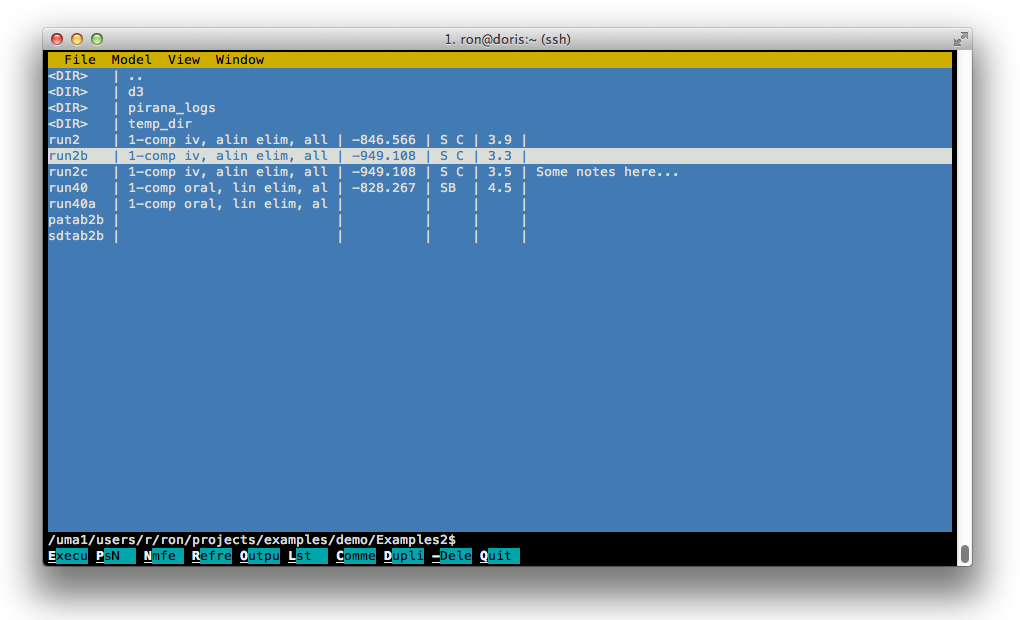
\includegraphics[scale=0.3]{images/cpirana_main.png}
    \caption{cPirana interface example}
\end{figure}


\section{Installing cPirana}

\subsection{Starting cPirana}
Copy the contents of the linux installation zip-file file to a location on your system. Pirana is started using the command (assuming you installed it in the folder /pirana inside your home folder):

\begin{lstlisting}
perl ~/pirana/cpirana.pl
\end{lstlisting}

cPirana will use the current folder as it's working folder. To make cPirana more easily accessible, add it as an alias to your .bashrc file, i.e.

\begin{lstlisting}
alias cpirana="perl ~/pirana/cpirana.pl"
\end{lstlisting}

Now you can browse to any folder, and start the program from there
using the {\ttfamily cpirana} command.

\vspace{10pt}
\noindent \scriptsize \textcolor{Blue}{Tip:} \textcolor{Grey} The manual section for cPirana is currently in development. Please check back regularly.
\normalsize


%%%%%%%%%%%%%%%%%%%%%%%%%%%%%%%%%%%%%%%%%%%%%%%%%%%%%%%%%%%%%%%%%%%%%%%%%%
\newpage  % one page left blank intentially
\thispagestyle{empty}
\mbox{}

\chapter{Validation}
Of course, the information gained from NONMEM or auxiliary tools must be
reliable and accurate. Validation of these tools is therefore an important consideration. 
The main aim of Pirana is to provide overviews of modeling results and
providing interfaces to other software (NONMEM, PsN, R, Xpose). As such, Pirana does not perform many calculations of its own. However,
Pirana does performs data parsing, formatting and reporting, i.e. in the creation of run reports. 

\noindent The Pirana development team has developed tools that perform a validation of parts of this
ecosystem. At current, we have two tools available:

\begin{description}
\item[valpsn] is a command-line tool that performs a
  series of pre-specified numerical tests, based on output from PsN
  tools. In the comparisons, the output from the specific PsN version
  that is to be validated (`test'-output) is compared to previously
  obtained output from a PsN version that is trusted, or has been
  validated in other ways (`reference'-output). The tools is
  scriptable, and includes R-scripts to perform the numerical
  comparison. It is however completely flexible, i.e. it allows custom
  R-scripts to be provided to perform the tests. The tool is currently
  not yet available from the Pirana website but can be supplied upon request.
\item[valpirana] is a command-line tool that perform a
  series of numerical test on the parameter estimates outputted by
  Pirana. The parameters ('test') are compared to those extracted by
  PsN's sumo tool (`reference'), for a user-specified library of
  models and modeling result files. This tool therefore solely focuses
  on Pirana and PsN's algorithms extraction of parameter estimates
  from NONMEM output files. Ultimately, this is Pirana's key feature,
  since Pirana does not perform many calculations, but is primarily a
  tool to generate overviews of results and allow the modeler to
  interpret results easier. The tool is currently
  not yet available from the Pirana website but can be supplied upon request.
\end{description} 

\noindent Note that both validation tools can be used to validate NONMEM as
well, e.g. if the reference output is obtained from a new, to be
validated, NONMEM version and compared to previously execute NONMEM
runs with a reference NONMEM version.

\vspace{20pt}
\noindent \textbf{IMPORTANT}: We do not claim any responsibility for the outcome
or validity of the validation analyeses obtained using these
tools. For example, we cannot guarantee that regulatory autharities accept
particular validations performed with these tools, nor do we claim the correctness of the validation results.
Please align intended validation procedure with the relevant authorities beforehand.

\section{Pirana validation tool}
While a few models and model outputs are supplied with the Pirana
validation tool, it is expected that the user provides a library of
models and NONMEM output files (usually .lst or .res files). The
Pirana validation tool expects a specific directory structure:

\begin{lstlisting}
\val_library
   - \res1
        - \model
   - \res2
   - \res3
\end{lstlisting}

\noindent The valpirana Perl script is invoked from the command line, using
e.g.:

\begin{lstlisting}
perl valpirana.pl -ini=val_pirana20130224.ini 
\end{lstlisting}

ValPirana will then read the ini-file, and loop (alphabetically)
through all folders in the folder specified in the ini-file. In each
folder, it will extract all parameter estimates and standard error
estimates (if available) using Pirana's internal NONMEM output parsing
routines. It will then run PsN's 'sumo' command, and store the
parameters outputted by PsN to memory as well. These will then be
compared, allowing for a pre-specified tolerance due to rounding.
The ini-file should be specified similar to:

\begin{lstlisting}
[general]
mod=mod
lst=lst
psn_dir=/usr/bin/
pirana_modules=/shared/val/pirana_modules_270
tol=

[lib1]
folder=/shared/val/valpirana_

[lib2]  # Optionally, specify multiple libraries
folder=
\end{lstlisting}

\subsubsection*{Pirana pre-release validation}
Before every Pirana release from version 2.4.0 upwards we used
(predecessors of) the valpirana tool to check that the parameter
estimates that Pirana extracts from NONMEM output files are exactly
the same as the ones reported by PsN's sumo command. For this
validation procedure we gathered more than 50 model and results files
from multiple modeling groups and many different modelers. While we cannot share the 
model and output in the validation library, if you
would like a report of the validation procedure, please contact us.

\section{PsN validation tool}
The PsN validation tool compares output from a `test'-installation of
PsN, with output from a trusted (previous) PsN installation. Tests can
be implemented for any of the tools in PsN (e.g. execute, bootstrap,
vpc, etc), and multiple tests can be performed for each tool
(recommended). The tests to be performed are specified in a setup file. Customizable
R scripts are used to perform the actual validation step for the tool. Every validation run is started by invoking the valpsn command:

\begin{lstlisting}
./valpsn ex1\_20130201.ini
\end{lstlisting}

\noindent This bash script invokes the main perl script that acutally performs the
validation. The script will read in the configuration file, and will
perform all the specified validation elements in the sequence
specified in the configuration file. The specific tests in the
validation run are all implemented in R scripts, and should output
SUCCESS or FAILURE. For every PsN tool a test script is provided with
the tool, but the user is encouraged to write custom scripts. 
More info is available in the specific manual for this tool (available upon request).

%%%%%%%%%%%%%%%%%%%%%%%%%%%%%%%%%%%%%%%%%%%%%%%%%%%%%%%%%%%%%%%%%%%%%%%%%%
\chapter{Endnotes}
\section{Acknowledgements} Many Pirana users are recognized for their
valuable suggestions and bug-reports, especially those in the Uppsala
and Amsterdam pharmacometrics groups.

\section{Bug reporting / suggestions}
If you find any bugs, please report them at the support section of our
website (http://www.pirana-software.com). A ticket will be created,
and we will get back to you as soon as possible. Please be as specific
as you can about the issue and report version number, system
characteristics, and if relevant provide screenshots and model/results
files. Requests of tips for further improvement of Pirana are very
welcome as well and can also be reported at the support section.

\section{Disclaimer} This software is provided under both an academic
and a commercial license. It is distributed on an `as is' basis,
without warranty of any kind. Your use of the software is at your sole
risk, and the authors cannot be held liable for any harm, inflicted
upon your system by this program. Any decision made on the basis of
output produced by Pirana is entirely your own responsibility. The
user is referred to the license for more information

\normalsize 



%%%%%%%%%%%%%%%%%%%%%%%%%%%%%%%%%%%%%%%%%%%%%%%%%%%%%%%%%%%%%%%%%%%%%%%%%%
\newpage  % one page left blank intentially
\thispagestyle{empty}
\mbox{}

\chapter{Tutorial: Pirana, PsN \& Xpose}

%!TEX root = manual_booklet.tex

\begin{center}
   {\colorbox{grey2}{
         \begin{minipage}[t]{0.9\textwidth}
The tutorial presented here is a tutorial on the use of PsN,
Xpose, and Pirana combined, and has been published before (\textit{\small Modeling \& 
simulation workbench for NONMEM: tutorial on Pirana, PsN and Xpose; Keizer RJ, Karlsson MO, Hooker AC}\normalsize, CPT-PSP 2013). 
The tutorial provides an excellent introduction to Pirana's basic
functionality, and its connections to the other tools. This
tutorial is aimed at modelers that have some familiarity
with NONMEM, but have no or limited experience with PsN or Xpose. The
training material and solutions are available from the Pirana website, or from CPT-PSP.
          \end{minipage}
      }
   }
\end{center}

\section{Introduction}
Several software tools are available that
facilitate the use of the NONMEM software and extend its
functionality. This tutorial shows how three commonly used and freely
available tools, Pirana, PsN, and Xpose, form a tightly integrated
workbench for modeling \& simulation with NONMEM. During the tutorial,
we provide some guidance on what diagnostics we consider most useful
in PK model development, and how to construct them using these
tools. 

\section{Background}Started in the early 80s with the development
of the NONMEM (acronym based on “NON-linear Mixed-Effects Modeling”)
software[1], “population analysis” has proven to be extremely useful
within pharmacometrics, both in the development of new drugs[2] and
the improvement of therapy with approved drugs.[3] Development of the
NONMEM software continues, and, although over time several other
modeling software tools have become available, NONMEM is still
regarded as the gold standard within the pharmacometric community: a
recent survey identified NONMEM (together with PsN[4]) as the most
frequently used software tool by far.[5] Modeling and simulation in
clinical pharmacology, and the use of NONMEM in particular, however,
has a steep learning curve for most starting researchers. This is
partially due to the fact that NONMEM is invoked from the command
line, and models are implemented using a Fortran-derived syntax
(NM-TRAN). Additionally, at its core, NONMEM performs only model
estimation (or simulation), and the implementation of essential
diagnostic tools such as bootstrap analyses and the creation of
goodness-of-fit plots are left to the modeler. Therefore, alongside
the development of NONMEM, many third-party tools have been developed
that facilitate the use of NONMEM by providing tools for organization
and automation. In this tutorial we will demonstrate the use of some
of the most widely used auxiliary software tools: PsN, Xpose[6], and
Pirana[7]. All three tools are released under an open source license
and are freely available (except for the commercial use of Pirana, for
which a commercial license is required). Separately, each tool offers
useful functionalities, but there is a synergistic benefit as well
when used together. 

The aim of this tutorial is to show how these three tools provide a
comprehensive workbench for modeling and simulation. This will be done
by showing examples of the most often encountered steps in PK model
development, i.e. a covariate modeling procedure and model evaluation
using residual- and simulation-based diagnostics. However, the aim of
the tutorial is not to provide guidance on how to perform a population
PK analysis, but strictly on these software tools. A detailed overview
of important aspects in population PK analyses has recently been
presented in this journal, and we refer the reader to that article for
guidance.[8] The current tutorial is structured in three parts: first
a brief introduction to these software tools is given, explaining
their basic purpose. In the main part of the tutorial, we show how a
typical PK model building analysis is performed with these tools and
NONMEM. At the end of the tutorial, several interesting additional
features are highlighted for each specific tool. We will assume the
reader is already somewhat familiar with NONMEM, although we have made
efforts to present and discuss the tools in a general fashion where
possible. All of the presented models, datasets, output, and
diagnostic plots are available in the online
materials.

\subsubsection{Software}
In this tutorial we will use NONMEM 7.2, Pirana
2.7.0, PsN 3.5.3, and Xpose 4.3.5. It is likely that future versions
will behave similarly, but in earlier versions not all functions
presented here may be available. We will show screenshots taken from
Windows, but all programs discussed here function similarly on all
major operating systems.

\begin{description}

\item [NONMEM] [9] is modeling software that allows the user to estimate
parameters in mixed-effects models (“population approach”) based on
maximum likelihood- or Bayesian techniques that use either gradient or
stochastic estimation methods. NONMEM translates model code written in
a unique Fortran-based syntax (NM-TRAN) into pure Fortran code, which
is then compiled and executed. NONMEM is currently developed by ICON
Development Solutions under a proprietary software license.

\item[PsN] [4] is a combination of tools for performing advanced modeling \&
simulation (M\&S) with NONMEM. It allows the implementation of
bootstraps, visual predictive checks and many other useful
functionality. PsN is written in Perl (and needs Perl installed,
freely available for all major operating systems), and is operated
from the command-line. Development started in 2000, and updates have
been released with regular intervals.

\item[Xpose] [6] is a tool for plotting and analyzing NONMEM output,
developed as a module for the R software (http://cran.r-project.org/,
open source, S-based statistical software). The tools in Xpose can be
used from the R command line or from a text-based menu system in
R. Xpose was first released in 1998, and was initially developed for
S-Plus. The current version (main version number 4) is however
released exclusively for R and builds upon the lattice module for
plotting. Both PsN and Xpose are developed at Uppsala University and
are released under an open-source license (GNU v2).

\item[Pirana] [7] is a graphical user interface for NONMEM, PsN and
Xpose/R. It has functionality for model management, model execution,
output generation, interpretation of results, and includes many other
tools. Development of Pirana started in 2007 at the Netherlands Cancer
Institute / Slotervaart Hospital (Amsterdam, NL), and is currently
continued by Pirana Software \& Consulting BV
(http://www.pirana-software.com). Pirana is released under an open
source license (Creative Commons) for academic users as well as a
commercial license. 

\end{description}

\section{Tutorial}In this tutorial, file and folder names are shown
in \fname{italic}, Pirana actions are shown \action{red-italic}, while commands,
arguments, NONMEM syntax and screen output are shown in \command{fixed-width
font}. We will step through an example model building exercise, with
the intent of showing how to create, manage, and evaluate
pharmacokinetic (PK) models for a given dataset. The PK dataset used
in this tutorial (\fname{pktab1}) is available in the on-line material, and
contains plasma concentration data obtained from a simulated clinical
trial of a novel iv drug, performed in 50 patients, measured at 8 time
points. All model files that are mentioned in this article are also
available on-line and can be used as reference. Make sure that all
software is installed correctly, and NONMEM runs can be started from
both PsN and Pirana (visit the respective websites for installation
instructions), and that the Xpose4 package is installed in R. Create a
folder for this analysis somewhere on your hard-drive, and put \fname{pktab1}
in this folder. Browse to this folder in Pirana, and save it as the
project “TutorialPSP” (\action{button 4 in figure 1}). As starting point for
NONMEM models, it is often easiest to use the PK model wizard in
Pirana, or start from one of the models available in the model
library. Start the wizard dialog window in Pirana (\action{Tools $\rightarrow$ Wizards})
and choose the PK model wizard, and explore the options. However, for
this tutorial we have already provided the first model (run1.mod):
copy the model run1.mod from the online material to the folder you
created. This model should now be visible in the Pirana main model
list when you direct Pirana to the right folder (if not, refresh
\action{Pirana button 5 in figure 1}). 

\begin{figure}[H] \centering
    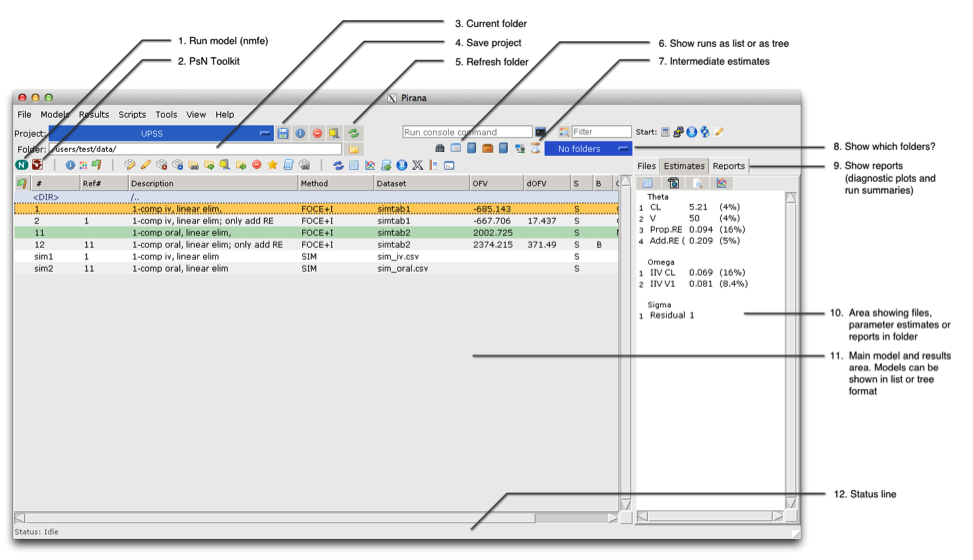
\includegraphics[scale=0.65]{images/fig1_Pirana_main.png}
    \caption{Pirana main screen}
\end{figure}

If you run from a model created by the wizard, make sure that the columns in the dataset match up exactly
with the records specified in the \$INPUT record in the model file. For
the provided run1.mod this has already been done. 

\subsubsection{First runs}If we would invoke the native NONMEM run script, we would run e.g. 

\begin{lstlisting}
nmfe72 run1.mod run1.lst
\end{lstlisting}

\noindent but Pirana automates this in a dialog window:
(\action{select model $\rightarrow$ right click $\rightarrow$ NONMEM $\rightarrow$ nmfe}). 
Several options are available to configure how and where (local or on a cluster) to run
the model, or whether to submit it to a job scheduler. If you choose
to run your models in Pirana through nmfe, you need to configure a
NONMEM installation in Pirana (\action{Settings $\rightarrow$ NONMEM}). Select the
quick-find option to scan your hard-drive for common installation
locations for NONMEM. If NONMEM is not found there yet, specify the
location yourself. 


In this tutorial we will however not use nmfe, but only PsN to run
models. There are multiple benefits of using PsN’s execute over the
regular nmfe command, the main ones being that models are run in
separate folders, runs can be restarted automatically upon crashes and
unsuccessful minimizations, and initial estimates can be
tweaked. Select the model and \action{right click $\rightarrow$ PsN
$\rightarrow$ execute}. Pirana will show a similar dialog window as
shown for nmfe, but now the command line for PsN’s execute tool is
shown (figure 2). For our first run, we will use the default command:

\begin{lstlisting}
execute run1.mod
\end{lstlisting}

\noindent After clicking the run button, if PsN and Pirana are
set up correctly, a console window will open with the following
message:

\begin{lstlisting}
Starting 1 NONMEM executions. 1
in parallel.
S:1 .. 
\end{lstlisting}

\noindent which indicates that one model estimation has
been started. The actual NONMEM process will run in a subfolder
created by PsN. By default this will be \fname{/modelfit\_dir1}, but a custom
folder name can be specified using the \command{-dir} argument. If the argument
\command{-model\_dir\_name}is specified, PsN will automaticlly choose an
informative foldername, in this case \fname{/run1.mod.dir.1}. 

\begin{figure}[H] \centering
    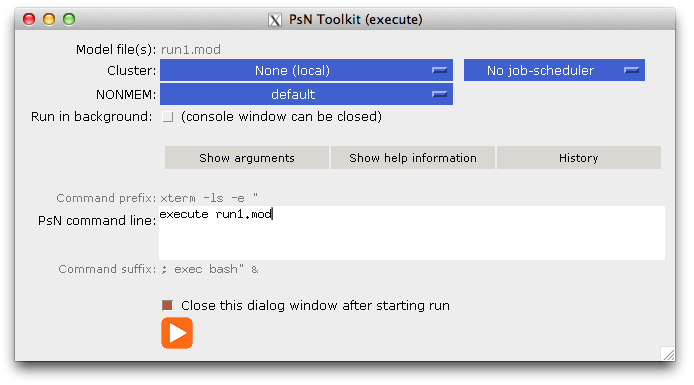
\includegraphics[scale=0.4]{images/fig2_psn_execute.png}
    \caption{PsN dialog window}
\end{figure}

\noindent Check that inside the folder created by PsN, a subfolder is created in which the
NONMEM process actually runs (\fname{/NM\_run1}). In Pirana, PsN folders are
hidden by default, as they may quickly clutter the model overview. To
unhide them again, select either “PsN folders” or “All folders” from
the folder selector (button 7 in figure 1). Many additional arguments
can be supplied to PsN commands to customize how PsN runs the NONMEM
model, e.g.: 

\begin{lstlisting}
execute run1.mod -dir=test1 –retries=3 -parafile=mpi6.pnm 
  –nm_version=nm72
\end{lstlisting}

\noindent which will run model run1.mod in the folder \fname{/test1}. PsN is
also instructed now to run using NONMEM version 7.2, parallelized
using MPI (specified in configuration file mpi6.pnm), and to retry
three times if the model doesn’t converge in the initial run, each
time changing the initial estimates of the parameters. A list of all
available arguments including help information is available from the
PsN dialog window in Pirana (figure 2), which is similar to using the
\command{-h} and \command{–help} arguments on the command line. In the PsN configuration
file (\fname{psn.conf}), a list of default arguments can be supplied as well,
so commonly used arguments do not have to be repeated on the command
line.

\subsubsection{Results evaluation} After estimation has completed,
refresh the Pirana main overview again. Basic results are now shown
for the run, such as the objective function value (OFV), whether
minimization was successful (S), and whether the covariance step was
successful (C). If the run was successful, PsN will automatically copy
back the results file (\fname{run1.lst}) and the produced output tables
(sdtab1, patab1) to the parent folder, which are then parsed by Pirana
upon refreshing. Select the model again, and now select the \action{Estimates
tab} from the right section of the Pirana window (11 in figure 1). The
right section will then show the parameter estimates for this run. A
more detailed overview that will e.g. show full random effect blocks
can be opened from here. Create a run summary in Word format
(alternatives are HTML, plain text or LaTeX), from the \action{menu $\rightarrow$ Results
$\rightarrow$ Run Reports $\rightarrow$ Word}. 

Diagnostic plots are a main decision tool in pharmacometric model
development, in which a distinction can be made between residual-based
diagnostics (goodness of fit plots based e.g. on residuals plotted
versus time or model predictions), and simulation-based diagnostics
(e.g. visual predictive checks, VPC). Obviously no strict rule should
be applied here, but in our experience residual-based diagnostics are
more useful in the first stages of model development, while
simulation-based diagnostics are more useful in the latter stages of
model development. Depending on what part of the model is diagnosed,
different diagnostic plots will be useful, and most likely no single
plot will suffice to evaluate model fit. Suggestions for diagnostic
plots for specific model parts are shown in table 1. Note that this
list is not exhaustive, and in addition, more specific plots may be
required for appropriate diagnosis.

\begin{figure}[H] \centering
    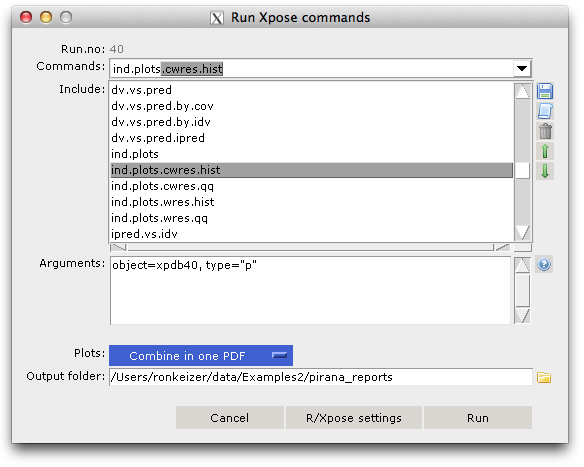
\includegraphics[scale=0.4]{images/fig3_xposeGUI.png}
    \caption{Xpose dialog window}
\end{figure}

For the current analysis, we will first have a look at some basic,
residual-based goodness of fit plots. A general model diagnostic is
the plot of weighted residuals versus time, or versus model
predictions. For models run with the conditional estimation method
(FOCE), it is most appropriate to use conditional weighted residuals
(CWRES, [10]). 

\begin{landscape}
\begin{table}[ht]
\caption{Suggested diagnostic plots in Xpose for PK development}
\vspace{10pt}
\footnotesize
\begin{tabular}{ p{4cm} p{12cm} }
Residual error model &
\begin{itemize}
\item Individual weighted residuals versus individual predictions (absval.iwres.vs.ipred)
\item Distribution / qq-plot of IWRES (iwres.dist.hist/qq)
\item In case of shrinkage: CWRES (cwres.dist.hist) or IWRESnpde 
\item Autocorrelation in residuals (autocorr.iwres)
\end{itemize} \\
Between subject variability model &
\begin{itemize}
\item Distribution / qq-plot of EBE’s (parm.hist.hist/qq)
\item In case of shrinkage: distribution of EBE$_{npde}$
\item Correlation between parameters (parm.splom)
\end{itemize} \\
Inter-occasion variability model &
\begin{itemize}
\item EBE parameter values vs occasions
\item Distribution / qq-plot of EBE (parm.dist.hist/qq)
\item In case of shrinkage: distribution of EBE$_{npde}$
\end{itemize} \\
Absorption model] &
\begin{itemize}
\item Individual profiles (ind.plots)
\item CWRES vs time after dose (cwres.vs.tad)
\item Individual g.o.f. plots (dv.vs.pred.ipred.by.idv)
\item Distribution of absorption parameters (ka, MTT, F) (parm.hist)
\end{itemize} \\
\end{tabular}
\end{table}
\end{landscape}

\begin{landscape}
\footnotesize
\begin{tabular}{ p{4cm} p{12cm} }
Disposition model & 
\begin{itemize}
\item Residuals versus time (cwres.vs.idv)
\item Individual profiles (ind.plots)
\item VPC (xpose.VPC)
\end{itemize} \\
Covariates &
\begin{itemize}
\item Parameter (EBE) vs covariate (parm.vs.cov)
\item In case of shrinkage: EBEnpde vs covariate 
\item G.o.f. plots by covariate (dv.pred.vs.idv.by.cov)
\item Correlations between covariates (cov.splom)
\item Influential individuals (dOFV.vs.id)
\item VPC stratified by covariate (xpose.VPC)
\item VPC with covariate as IDV (xpose.VPC)
\end{itemize} \\
\end{tabular}
\end{landscape}
\normalsize

\noindent Use the Xpose GUI within Pirana to create these plots:
\action{select model $\rightarrow$ right click $\rightarrow$ Xpose
$\rightarrow$ Xpose GUI}. Add the plot \command{cwres.vs.pred} and \command{cwres.vs.idv}
to the list of plots, and possibly some additional goodness-of-fit
plots (a list of useful Xpose plots is given in table 2). In these
plots you should observe an obvious pattern in the residuals. It may
not be obvious immediately what is the cause of the misspecification,
but a look at the individual plots (\command{ind.plots}) probably gives more
insight: the model seems to be missing the bi-phasic nature of the
observed data. Therefore, in the next step we will add distribution of
drug into a peripheral compartment to our PK model, but first we will
briefly discuss how to keep track of model development

Besides the Xpose GUI, there are several alternative ways of creating
diagnostic plots from Pirana:

\begin{itemize}
\item DataInspector: a quick and flexible method for creating
  diagnostic plots based on NONMEM output, or checking input
  datasets. Select the DataInspector for \fname{run1.mod} (\action{right click
  $\rightarrow$ Model $\rightarrow$ Open DataInspector}). Pirana will
  ask you now which input- or ouput file to open, choose the file
  sdtab1. In the DataInspector window, the variables on the x- and
  y-axis can be easily changed to any variable in the dataset, and
  filters can be applied on patient ID, or on any other variable. From
  this window, R-code can be generated that will recreate the same
  graph in R.
\item R script library: Pirana comes bundled with a library of
  diagnostic R scripts, which can be run automatically from
  Pirana. Select a model and select the one of the R-scripts from the
  Scripts Tab, e.g. \action{Basic GOF $\rightarrow$ DV vs IPRED}, and then
  select Run script from the buttons above the list. The requested
  plot will be created in a PDF document and opened. Created plots
  will be listed in the “Reports” tab (10 in figure 1). The standard
  scripts bundled with Pirana can be extended and customized easily,
  but that is beyond the scope of this tutorial. Please refer to the
  manual and default scripts for guidance.

\item Xpose menu system in R: The Xpose menu system can be started
  from Pirana (\action{right click $\rightarrow$ Xpose $\rightarrow$ Start
  Xpose menu in R}), or manually from an R session by
  invoking:
  \begin{lstlisting}
    library(xpose4)
    xpose4()
  \end{lstlisting}

  Xpose will then ask for the run number, which is used to determine
  which tables to import. Note that to use Xpose, NONMEM needs to be
  instructed to output tables that adhere to a specific naming and
  structure (see online materials table I, or the Xpose website). If
  you didn’t use the Pirana model wizard to create the tables, add
  them manually in the NONMEM model file, using e.g.:

\begin{lstlisting}
$TABLE ID TIME IPRED IWRES EVID MDV 
       NOPRINT ONEHEADER FILE=sdtab1
\end{lstlisting}

From the Xpose menu system, goodness-of-fit plots can
be created, e.g. browse to 

\begin{lstlisting}
4: Goodness of fit plots
2: Basic goodness of fit plots
\end{lstlisting}

\end{itemize}

\begin{landscape}
\begin{table}[ht]
\caption{Commonly used arguments for Xpose functions}
\vspace{10pt}
\footnotesize
\begin{tabular}{ p{3.1cm} p{9cm} p{4.5cm}}
\textbf{Function} & \textbf{Description} & \textbf{Commonly used arguments} \\ 
basic.gof & Compound plot of basic goodness-of-fit plots & use.log, force.wres\\
y-var.vs.x-var & General diagnostics functions: y-var can be one of dv, pred, ipred, iwres, cwres, wres. x-var can be any of pred, ipred, idv. Add “.by.cov” or “.by.idv” to the command to split the plot by covariate or by individual. & abline, smooth\\
ind.plots & Plots of dv, pred and ipred versus time, split by individual. & y.vals, layout\\
xpose.VPC & Visual predictive check (uses PsN output folder) & VPC.info, VPCtab, PI.ci, PI.real, type\\
xpose.VPC.categorical & Visual predictive check for categorical data & level.to.plot, max.plots.per.page\\
xpose.VPC.both & Visual predictive check for continuous and categorical data (e.g. BLOQ data) & See above\\
autocorr.cwres & Plot cwrest+1 vs cwrest to check for autocorrelation in residuals & type, smooth, ids\\
parm.hist / parm.qq & Plot distributions / qq-plots of model parameters & onlyfirst\\
parm.vs.parm & Plot model parameter versus model parameters & onlyfirst, abline, smooth\\
parm.vs.cov & Plot parameters and eta’s versus covariates to check for correlation & onlyfirst, smooth\\
xpose.gam & Generalized Additive Models (covariate model building tool) & parnam, covnams, start.mod\\
basic.model.comp & Compare basic goodness-of-fit plots between two models & object.ref\\
kaplan.plot & Visualizes data and VPC from survival models & x, y, id, data, by \\
\end{tabular}

\bigskip

\textit{
\noindent For most functions listed above, the following general arguments are useful: object (which Xpose database to use), main (plot title), inclZeroWRES (include values where WRES is zero).\\
\noindent In R, help information for functions can be obtained by giving the command ?<function>, where <function> is the  desired R/Xpose function. \\
\noindent Abbreviations: dv = dependent variable, idv = independent variable, (c/i)wres: (conditionally / individual) weighted residuals. pred = population predicitions, ipred = individual predictions.
}
\end{table}
\end{landscape}

\subsubsection{Model management in Pirana}
In M\&S projects in both academia and industry, it is essential to
keep track of the model development history. Pirana and PsN offer a
tool to aid the modeler with this through the run record. The run
record entails a standardized way of keeping track of model meta
information such as the “parent” model, a description and/or a label
for the model, and other information about the model components. We
consider it good modeling practice to create a new model file for
every change that is made to a model. 

Duplicate the first model in Pirana (\action{right click on \fname{run1.mod} 
$\rightarrow$ File actions $\rightarrow$ duplicate}). In the dialog
that will open up, \fname{run2.mod} is suggested as new model file name, and
we can select which model is the reference model for this model
(\fname{run1.mod}), and optionally update the initial estimates with the
parameter estimates from the reference model. The model description
and other meta-information is stored in the model file itself using
the run record syntax (also see the userguide for the run record on
the PsN website). Pirana can show the main model overview as a list or
as a tree (button 6 in fig 1), and can export a copy of the run record
to various formats including comma separated (\fname{csv}) files, HTML files
and Word documents (\action{Results $\rightarrow$ Run records}), or create an
interactive visualization of the model development tree or “visual run
record”[11] like shown in figure 4 (\action{Results $\rightarrow$ Run records
$\rightarrow$ Visual run record}).

\begin{figure}[H] \centering
    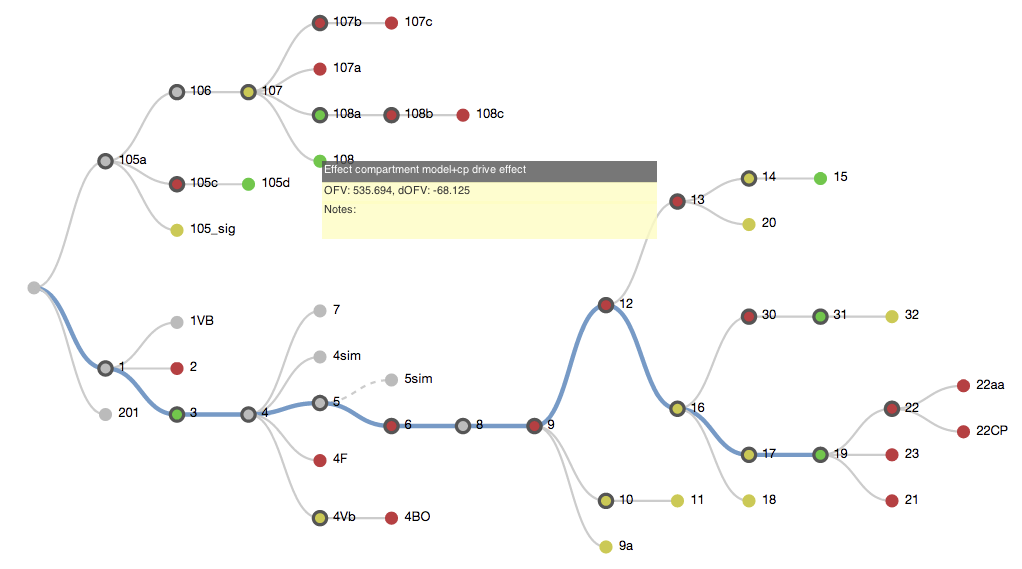
\includegraphics[scale=0.3]{images/fig4_vrr.png}
    \caption{Visual Run Record}
\end{figure}

After duplication, the model \fname{run2.mod} will be shown in the model
overview, and opened in the editor, where we will now add a peripheral
compartment to the model error model: change \$SUBROUTINE to use ADVAN3
and TRANS4, change the parameter V into V1, and add to \$PK: 

\begin{lstlisting}
Q = THETA(3)
V2 = THETA(4)
\end{lstlisting}

\noindent Of course, initial estimates for the intercompartmental distribution
(Q) and peripheral compartment (V2) have to be specified as well in
\$THETA. For now we chose to run this model without IIV on these
parameters. Run this model using execute, evaluate the drop in
objective function, and compare the diagnostic plots for run2 to those
made for run1. You should encounter a considerable drop in the
objective function value, and find that the diagnostic residual plots
show much improved model fit. 

Next, we will diagnose the residual error model, for which an
important diagnostic plot is that of absolute individual weighted
residuals ($|$IWRES$|$) versus individual predictions (IPRED). For a true
model, the distribution of absolute residuals should be similar over
the whole range of the x-axis variable. If a homoscedastic error
structure (additive error) was implemented in \fname{run1.mod} and \fname{run2.mod},
the plot will show larger residuals at higher individual 
predictions. This should therefore lead you to conclude that a
heteroscedastic (combined proportional and additive) error model
should provide a better description of the data. Therefore, create a
new model (run3.mod) based on run2.mod and implement a combined error
model using e.g.: 

\begin{lstlisting}
Y = IPRED * (1+EPS(1)) + EPS(2)
W = SQRT(IPRED**2*SIGMA(1,1)**2 + SIGMA(2,2)**2)
IWRES = (DV-IPRED)/W
\end{lstlisting}

\noindent It must be noted that the plot mentioned above is only
informative at low ε-shrinkage (as a rule-of-thumb, at $\epsilon$-shrinkage $>
~5\%$ this plot loses informativeness).[12] In cases of higher
shrinkage, plots of CWRES versus individual predictions (IPRED), or
IWRES$_{npde}$ [13] versus IPRED are more informative. The diagnostic plots
as well as the significant drop in OFV indicate that the combined
error model provides better fit. 

\subsubsection{Covariate model}
The dataset \fname{pktab1} contains three continuous covariates: weight (WT),
creatinine clearance (CRCL), AGE, and two binary covariates: SEX and
study center (CENT). Since the number of covariates is low (5), one
might choose to test these covariates manually. However, in the next
step of this tutorial we will perform stepwise covariate modeling
(scm) in PsN, to demonstrate this automated method. In the first phase
of the scm, covariates are added to the base model in a stepwise
fashion based on statistical significance (decrease in OFV). In a
second “backward elimination” phase, covariates are then removed from
the final model obtained in the first phase, if removal of the
covariate does not result in significantly worse fit. The backward
step is typically done at a higher significance level. Like all PsN
tools, the scm can be run from the command line or from Pirana, in a
similar way as done before for execute. However, the scm tool requires
that a configuration file is created first. Several examples of
configuration files are available on the PsN website, but here we will
create one using the wizard in Pirana (\action{Tools $\rightarrow$ Wizards
$\rightarrow$ scm configuration file}).  Create a configuration file,
with the filename \fname(psp.scm), in which all covariates are tested on both
CL and V1, at a significance level of 0.1 (forward step) and 0.05
(backward step) and restrict the analysis to linear relationships (set
the relationships argument to “1,2”). Check that the correct
covariates are included; the ones shown in the wizard are only
placeholders. If you’re not sure on the correct syntax of the scm
file, please have a look at the provided annotated configuration file
(psp.scm in the on-line appendix). Before starting the scm, duplicate
run3.mod to run4.mod, and remove any \command{\$TABLE} records that are
present. Start the scm from the PsN dialog window using this command:

\begin{lstlisting}
scm psp.scm –model=run4.mod
\end{lstlisting}

\noindent After the scm has completed, PsN will compile an output file
called \fname{scmlog.txt} in the scm folder. Open this file and interpret the
information, it holds the results for all tests performed in the scm
and shows how the final covariate model was constructed. You should
find that 4 covariate relationships are significant: CRCL on CL, WT on
CL, WT on V, and SEX on V. This will be our “final model” from the
covariate model-building step. If you did not find these results,
compare your results with those provided in the on-line
appendix.

More elaborate covariate model building techniques based on the scm
are available in PsN as well, such as the cross-validated scm
(\command{xv\_scm})[14], and the bootstrap of the scm (\command{boot\_scm})[15]. These tools
provide more details on the predictive ability of the model, and on
selection bias and expected covariate model size, respectively. They
can also be run on linearized versions of the model, to reduce the
computational workload.[16] Other covariate modeling tools that are
available in PsN include the lasso[17] and the fixed random effects
model (FREM, [18]), while in Xpose the gam and bootstrap of the gam
(bootgam) are implemented [6]. All of these methods have certain
advantages and drawbacks, which are however beyond the scope of this
article.

\subsubsection{Final model}
If the scm completed successfully, you will find a folder called
\fname{final\_models} inside the scm folder created by PsN. Inside that folder,
locate the final model with included covariate relations and copy that
to the main model folder, renaming it to \fname{run5.mod}. We will use this
model to perform some more elaborate diagnostic evaluation, i.e. we
will get bootstrap estimates for our parameters and create a VPC. So
first open the PsN bootstrap dialog window (\action{Right click $\rightarrow$
PsN $\rightarrow$ Model diagnostic $\rightarrow$ bootstrap}). A
required argument to the bootstrap command is the –samples argument,
which specifies how many bootstrap samples should be drawn. More
samples will make the bootstrap estimates and percentile estimates
more precise, however at the expense of increased computation
times. The recommended number of samples for an analysis will depend
on what statistic is desired by the modeler. For obtaining bootstrap
means of the parameter estimates, 100 samples may be enough, but to
obtain accurate 5th and 95th percentiles, 1,000 or more are required
to obtain precise estimates. After the bootstrap is finished (on a
single core, a bootstrap of 200 samples may easily take an hour for
this model), the results from the bootstrap are available in the
bootstrap folder, in the files \fname{raw\_results\_run5.csv} and
\fname{bootstrap\_results.csv}. Open these files and interpret the output: are
the parameters estimated with adequate precision? In Pirana, select
the bootstrap folder created by PsN and run the R-script to create
plots of parameter distributions (\action{Scripts tab $\rightarrow$ PsN
$\rightarrow$ Bootstrap results}), which facilitates evaluation and
interpretation of these bootstrap results. 

Earlier in this tutorial we presented how basic goodness-of-fit plots
can be created in Pirana and Xpose. Now we will use all three tools to
create a visual predictive check (VPC) of the final model
(run5.mod). A VPC is an internal validation tool, i.e. it shows how
well the model predicts the data on which the model was
conditioned. It visualizes the median model prediction, the
variability between patients and within patients (5th and 95th
percentiles), and the uncertainty around the predicted
percentiles.[19] Before we create a VPC, we would like to stress a few
points. Firstly, in VPCs it is important to show the uncertainty
around the model predicted percentiles, instead of presenting only
lines indicating the point estimates of the percentiles. Signs of
model improvement are when the confidence areas of the simulated
percentiles encompass more of the observation percentiles, but also
when the confidence intervals themselves are shrinking (while still
encompassing the observation percentiles).  Furthermore, since the VPC
shows summary statistics (percentiles) of observations and predictions
for binned data, the “binning method is an important consideration. To
avoid inflation of the uncertainty around the summary statistics, each
bin should contain an adequate amount of observations. A quick
rule-of-thumb is that there should not be more bins than the number of
observations per individual. PsN currently incorporates several
binning approaches: manual bin specification (\command{-bin\_array=x,y,z,etc}),
binning into an equal number of datapoints per bin (\command{-bin\_by\_count=1
–no\_of\_bins=\#}), or spacing the bins equally over the x-axis
(\command{-bin\_by\_count=0}, \command{-no\_of\_bins=\#}). Importantly, binning across a large
variability in dose and/or influential covariates can diminish the
diagnostic value of a VPC. One approach to overcome this is to
stratify the VPC by the covariate, but this is not always possible
e.g. due to limited data per stratum. Also when data arises from
studies with adaptive designs (e.g. dose adjustments), VPCs are
misleading unless the adaptation protocol is included in the
model. The prediction-corrected VPC (pcVPC) offers a solution to these
problems while retaining the visual interpretation of the traditional
VPC.[20] pcVPCs can be constructed by adding the argument \command{–pred\_corr}
to the PsN VPC command.

\begin{figure}[H] \centering
    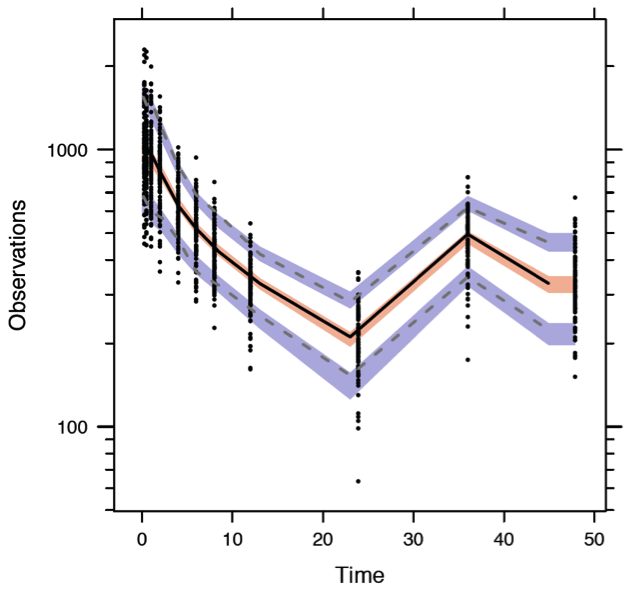
\includegraphics[scale=0.8]{images/fig5_vpc.png}
    \caption{Visual Predictive Check (vpc)}
\end{figure}

VPCs can be made in Pirana using the PsN dialog window (\action{right click
$\rightarrow$ PsN $\rightarrow$ model evaluation $\rightarrow$ VPC}),
or from the command line. As discussed above, essential arguments to
pass to the VPC are the number of samples and the binning
method. Increasing the number of samples will increase the accuracy of
the summary statistics for the simulation and their uncertainty
interval (but it will not decrease the uncertainty interval
itself). Start the VPC tool using:

\begin{lstlisting}
  vpc –samples=500 –no\_of\_bins=8 –bin\_by\_count=1 run5.mod
\end{lstlisting}

The first of the two NONMEM runs that are started will only output a
table with the necessary (observation) data for the VPC, it does not
perform parameter estimation. The other model runs repeated Monte
Carlo simulations of the model, using the same dataset design as the
original. After the two NONMEM runs have finished, PsN will process
the output, bin the simulated and observed data, calculate the
percentiles and confidence intervals for each bin, and export a
csv-file with the summary statistics. This csv-file can then be
processed by Xpose and turned into a VPC-plot, which can be automated
from Pirana using the Xpose GUI as described before, or using the R
scripts library. Both approaches will create and open a pdf-file with
the VPC (see example in figure 5). Using the latter approach this is
done as follows: select the VPC-folder created by PsN, and open the
Scripts tab on the right. In the list of R scripts, choose \action{Xpose
$\rightarrow$ VPC $\rightarrow$ Basic\_log\_y.R}. A pdf-file with the VPC
will be generated and opened from Pirana. As an exercise, try to
create the same plot using the Xpose GUI in Pirana as well: select the
model in the main overview, and \action{right click $\rightarrow$ Xpose
$\rightarrow$ Xpose GUI}. Since only limited space is available for
this tutorial we will not demonstrate other diagnostics. We will
however create a run record of the model development: in the menu bar
click \action{Results $\rightarrow$ Run records $\rightarrow$ Detailed run
record (csv)}. This will create and open a csv-file containing run
numbers, descriptions, other meta-information and run results. If the
file does not open automatically, please look it up in the “Files” tab
on the right and double click it. As a final step in our PK model
development, select the final model again and bundle that model file,
the associated result files and output files and the VPC folder into a
zip-file (\action{Right click $\rightarrow$ File actions$\rightarrow$ Compress
to zip-file}). Also create a bundled report of the goodness-of-fit
plots for the final model (in the Reports tab select the desired pdf’s
and click \action{Bundle into... $\rightarrow$ $<$output format$>$}). 

\subsubsection{Additional features}
For all three software tools presented here, we have only scratched
the surface of possibilities. The reader is encouraged to explore more
advanced functionality using the documentation available on the
respective websites. We will highlight a few examples of more advanced
features for the three programs below.

\begin{description}
\item[PsN] the simulation and re-estimation (\command{sse}) tool can be used to
  evaluate trial designs, e.g. to evaluate whether model parameters
  can be estimated with adequate precision under the intended or
  alternative experimental designs or with alternative models. It is
  also useful for evaluating fundamental modeling aspects, e.g. to
  evaluate how model diagnostics perform under given designs. Another
  interesting tool for design evaluation, specifically for the
  calculation of study power and number of study subjects required, is
  Monte Carlo Mapped Power (\command{mcmp}).[21] In this tool, which is also
  based on simulation and re-estimation, the individual objective
  function values calculated in NONMEM are exploited to evaluate
  designs in a more rapid way than using sse. Case deletion
  diagnostics (\command{cdd}) is a tool that can be useful in the final stages
  of model development, to investigate whether model fit depends more
  heavily on particular strata of the dataset. The most important PsN
  functions are listed in table 3.
\item[Xpose] In this tutorial we showed how to create goodness-of-fit
  plots from the Xpose menu system, and from the Xpose interface in
  Pirana (VPC). However, the most efficient way to use Xpose,
  especially when doing repetitive jobs, is to use scripts to create
  the desired goodness-of-fit plots. A list of useful Xpose functions
  is given in table 2, while a more complete overview of functions and
  example scripts (“bestiarium”) is available on the Xpose
  website. The default plots in Xpose can be extended and modified in
  various ways. Firstly, most Xpose functions take arguments that
  alter the implementation of the plot. The looks of the plots can
  also be changed by directly passing lattice arguments to the Xpose
  function. Secondly, the input variables can be altered easily to
  allow creation of non-default plots. E.g. to create a plot of a
  covariate METAB vs IDV instead of DV vs IDV we can ‘trick’ Xpose
  into using METAB as DV while maintaining the plot
  characteristics:
\begin{lstlisting}
> change.xvardef(xpdb, "dv") <- c("METAB")
> xplot <- dv.vs.idv(xpdb)
> print(xplot)
\end{lstlisting}

\noindent Finally, since Xpose is an open source R module, it is possible to
modify the Xpose functions directly, if further modifications are
required.

\item [Pirana] a model translator is included that can translate
any NONMEM model (written in an NM-TRAN ADVAN subroutine), to
differential equation code for R (using deSolve library), Berkeley
Madonna (software dedicated to ODE simulations), or Matlab / PopED
[22]. Note that many functions in Pirana can be extended and
customized by the user, such as the R-scripts library and the
wizards. Pirana can also be used for modeling on remote clusters
(through ssh-connections), and has native support for SGE, Torque and
Condor job schedulers.

\end{description}

\begin{landscape}
\begin{table}[ht]
\caption{Commonly used PsN tools}
\vspace{10pt}
\footnotesize
\begin{tabular}{ p{3.1cm} p{6cm} p{7.5cm}}
\textbf{Tool command} &  \textbf{Description} & \textbf{Commonly used arguments}\\
execute & Run a model in NONMEM & -retries –picky –model\_dir\_name \\
VPC & Visual predictive check & -samples -bin\_by\_count –no\_of\_bins –bin\_array –dv -idv\\
bootstrap & Run a bootstrap & -samples –stratify\_on \\
cdd & Case deletion diagnostics & -samples –case\_column \\
sse & Simulation and (re-)estimation & -samples –alternative\_models –no-estimate\_simulation \\
mcmp & Monte Carlo Mapped power & -n\_bootstrap –start\_size –increment -df \\
scm & Stepwise covariate modeling & -config\_file –model \\
xv\_scm & Cross-validated stepwise covariate modeling & -config\_file –max\_steps -splits \\
boot\_scm & Bootstrap of stepwise covariate modeling & -config\_file -samples –dummy\_covariates -run\_final\_models \\
llp & Log-Likelihood profiling and maximum-likelihood parameter estimates & -ofv\_increase –thetas –omegas –max\_iterations \\
psn\_options & Shows all general PsN options & -nm\_version -verbose \\
update\_inits & Updates initial estimates based on a NONMEM output file from a previous run & -from\_model –output\_model \\
lasso & the Lasso (covariate modeling) & -relations –lst\_file \\
mimp & Multiple imputation (missing data method) & -base\_model –reg\_model –mi\_model -imputations \\
General options* & Applies to every PsN tool  & -clean \\

\end{tabular}

\bigskip

\textit{
\noindent For each tool, the arguments –h and –help show a list of arguments and a detailed description of the arguments, respectively. \\
\noindent Note that arguments can also be set in the psn configuration file. 
In that case they don’t have to be specified again on the command line.
}

\end{table}
\end{landscape}

\section{Conclusion} In this tutorial we presented a modeling
workbench that incorporates three tools, which in our view make M\&S
with NONMEM more powerful, more efficient and easier to perform. It is
our intention to implement all new modeling techniques and diagnostics
developed within our group into PsN, Xpose and/or Pirana, so new
versions are expected to be released on a regular basis.


\subsubsection{Conflict of Interest}RJK is owner of Pirana Software \& Consulting
BV, which provides commercial licensing of Pirana. MOK and
AH have no conflicts of interests.

\subsubsection{Acknowledgements}
The researchers in the Pharmacometrics Research Group are acknowledged
for their input on the use of diagnostics in model
development.


\subsection*{References}
\scriptsize 
\begin{enumerate}
\item Sheiner LB, Beal SL. Evaluation of methods for estimating
  population pharmacokinetics parameters. I. Michaelis-Menten model:
  routine clinical pharmacokinetic data. Journal of pharmacokinetics
  and biopharmaceutics [Internet] 1980 [cited 2012 Aug 3];8(6):553–71.

\item Stone JA, Banfield C, Pfister M, Tannenbaum S, Allerheiligen S,
  Wetherington JD, et al. Model-based drug development survey finds
  pharmacometrics impacting decision making in the pharmaceutical
  industry. Journal of clinical pharmacology [Internet] 2010 [cited
  2012 Aug 3];50(9 Suppl):20S–30S.

\item Zandvliet AS, Schellens JHM, Beijnen JH, Huitema ADR. Population
  pharmacokinetics and pharmacodynamics for treatment optimization in
  clinical oncology. Clinical pharmacokinetics [Internet] 2008 [cited
  2012 Aug 3];47(8):487–513.

\item Lindbom L, Pihlgren P, Jonsson EN, Jonsson N. PsN-Toolkit--a
  collection of computer intensive statistical methods for non-linear
  mixed effect modeling using NONMEM. Computer methods and programs in
  biomedicine [Internet] 2005 [cited 2012 Jul 25];79(3):241–57.

\item Vlasakakis G, Comets E, Keunecke A, Gueorguieva I, Magni P,
  Terranova N, et al. White paper: Landscape on technical and
  conceptual requirements and competence framework in Drug / Disease
  Modeling \& Simulation. CPT:PSP (In press)

\item Jonsson EN, Karlsson MO. Xpose--an S-PLUS based population
  pharmacokinetic/pharmacodynamic model building aid for
  NONMEM. Computer methods and programs in biomedicine [Internet] 1999
  [cited 2012 Aug 3];58(1):51–64.

\item Keizer RJ, Van Benten M, Beijnen JH, Schellens JHM, Huitema
  ADR. Piraña and PCluster: a modeling environment and cluster
  infrastructure for NONMEM. Computer methods and programs in
  biomedicine [Internet] 2011 [cited 2011 Jul 12];101(1):72–9.

\item Byon W, Smith MK, Chan P, Tortorici MA, Riley S, Dai H, et
  al. Establishing Best Practices and Guidance in Population Modeling:
  an Industry Experience with a Population Pharmacokinetic Analysis
  Guidance. CPT:PSP (In press)

\item Beal S, Sheiner LB, Boekmann A, Bauer RJ. NONMEM’s User's
  Guides. Ellicott City, Maryland, USA.: ICON Development Solutions;
  10.  Hooker AC, Staatz CE, Karlsson MO. Conditional weighted
  residuals (CWRES): a model diagnostic for the FOCE
  method. Pharmaceutical research [Internet] 2007

\item Keizer RJ. The Visual Run Record: visualization of the model
  development history. In: Abstracts of the World Conference on
  Pharmacometrics. Seoul, South-Korea: 2012.

\item Karlsson MO, Savic RM. Diagnosing model diagnostics. Clinical
  pharmacology and therapeutics [Internet] 2007 [cited 2012 Aug
  3];82(1):17–20.

\item Keizer RJ, Harling K, Karlsson MO. Extended NPDE diagnostics for
  the between-subject variability and residual error
  model. PAGE. Abstracts of the Annual Meeting of the Population
  Approach Group in Europe. 2012;21:Abstr 2538.

\item Katsube T, Khandelwal A, Harling K, Hooker AC, Karlsson
  MO. Evaluation of Stepwise Covariate Model Building Combined with
  Cross-Validation [Internet]. In: PAGE. Abstracts of the Annual
  Meeting of the Population Approach Group in Europe. 2011. page Abstr
  2111.

\item Keizer RJ, Khandelwal A, Hooker AC, Karlsson MO. The bootstrap
  of stepwise covariate modeling. In: PAGE. Abstracts of the Annual
  Meeting of the Population Approach Group in Europe. Athens, Greece:
  2011. page Abstr 2161.

\item Khandelwal A, Harling K, Jonsson EN, Hooker AC, Karlsson MO. A
  fast method for testing covariates in population PK/PD Models. The
  AAPS journal [Internet] 2011 [cited 2012 Aug 2];13(3):464–72.

\item Karlsson MO. A full model approach based on the covariance
  matrix of parameters and covariates. PAGE. Abstracts of the Annual
  Meeting of the Population Approach Group in Europe. 2012;21:Abstr
  2455.

\item A Tutorial on Visual Predictive Checks [Internet]. [cited 2012
  Aug 3]; http://www.page-meeting.org/default.asp?abstract=1434

\item Bergstrand M, Hooker AC, Wallin JE, Karlsson
  MO. Prediction-corrected visual predictive checks for diagnosing
  nonlinear mixed-effects models. The AAPS journal [Internet] 2011
  [cited 2012 Jul 17];13(2):143–51.

\item Vong C, Bergstrand M, Nyberg J, Karlsson MO. Rapid sample size
  calculations for a defined likelihood ratio test-based power in
  mixed-effects models. The AAPS journal [Internet] 2012 [cited 2012
  Aug 3];14(2):176–86.

\item Nyberg J, Ueckert S, Strömberg EA, Hennig S, Karlsson MO, Hooker
  AC. PopED: An extended, parallelized, nonlinear mixed effects models
  optimal design tool. Computer methods and programs in biomedicine
  [Internet] 2012 [cited 2012 Aug 13]
\end{enumerate}

\normalsize

%%%%%%%%%%%%%%%%%%%%%%%%%%%%%%%%%%%%%%%%%%%%%%%%%%%%%%%%%%%%%%%%%%%%%%%%%%

\clearpage
\chapter{Quick Guides}

\clearpage
\section{Quick Guide: Configuring Pirana }

\begin{center}
   {\colorbox{grey2}{
         \begin{minipage}[t]{0.9\textwidth}
\subsubsection*{Scope}
This Pirana Quick Guide explains how to configure the most important settings in Pirana. 
          \end{minipage}
      }
   }
\end{center}

Most of the settings for Pirana can be configured through the menu File $\rightarrow$ Settings. The following sections deal with the different sections of the Settings window.

\subsubsection*{General settings}
\begin{itemize}
\item The general settings window (Figure 1) deals with some of the general settings for working with Pirana.
\item Most of settings do not need altering to work with Pirana. The meaning of most important settings is discussed below:
\subitem \emph{Alternative data directory}: Alternative location for model input data files.
\subitem \emph{Enable nmfe runs}: If this option is selected, models can be run directly using nmfe.
\subitem \emph{Enable Pirana as wrapper for PsN/WFN/Monolix}: If these options are selected, Pirana may be used to run models through PsN or WFN. Monolix support is experimental.
\subitem \emph{Enable the use of PCluster}: Experimental feature, not supported (refer to PC cluster manual).
\end{itemize}


%% Fig 1 
\begin{figure}[h] \centering
    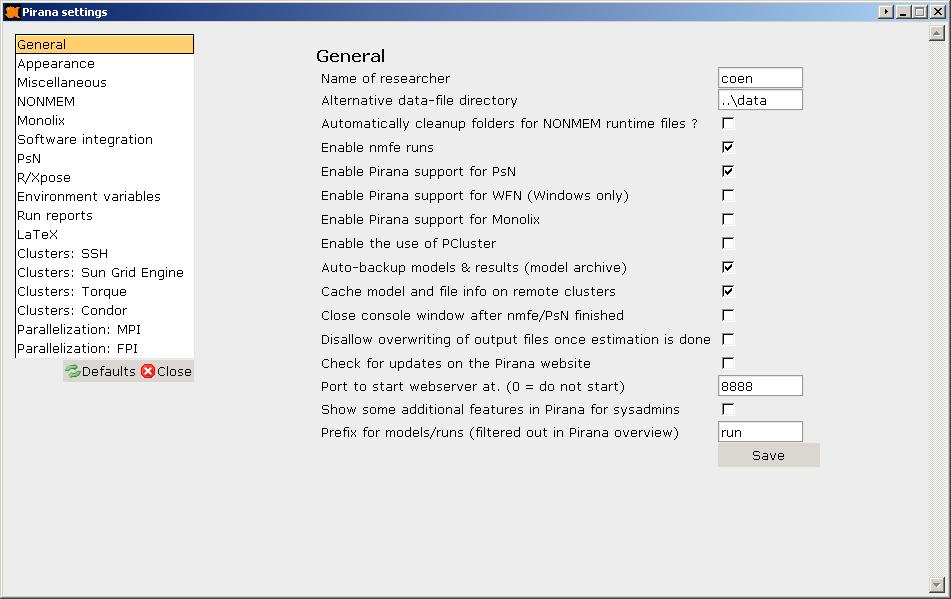
\includegraphics[scale=.4]{images/settings_1.jpg}
    \caption{General settings window}
\end{figure}

\subsubsection*{NONMEM}
\begin{itemize}
\item Refer to the NONMEM quick guide for detailed support on how to setup NONMEM instatllations. 
\item This is not necessery if PsN is used. 
\end{itemize}

\subsubsection*{Software integration}
\begin{itemize}
\item The software integration tab (Figure 2) deals with the integration of other software packages into Pirana. 
\item If the background of a software location appears green, the program can be found, whereas if it is red the program cannot be located under the specified path.
  \item Except for the list of programs defined below,  \emph{all other items in the software integration window are not necessery to define in order to work with Pirana}. Most other programs locations are only used to create easy links to the software from within Pirana. Also the location of \emph{psn.conf} is not needed to work with PsN.
 \item The following software packages are important to set correctly in order to work with Pirana easily: 
 \subitem \emph{R location}; Pirana uses R and Xpose to generate graphs, hence it is important to set the path to R correctly.
 \subitem \emph{Location of R GUI} (if available); if a GUI for R is available this should be specified. RStudio is recommended.
 \subitem\emph{ Spreadsheet location} (i.e. Excel, Numeric etc.), to view the contents of CSV files.
 \subitem\emph{ Code/text editor}; This editor will be used to edit models or scripts and is therefore important to define. 
 \subitem\emph{ PDF file viewer}; Many graphics are created as PDF files, hence a PDF viewer is useful to define.
\end{itemize}
%% Fig 2
\begin{figure}[h] \centering
    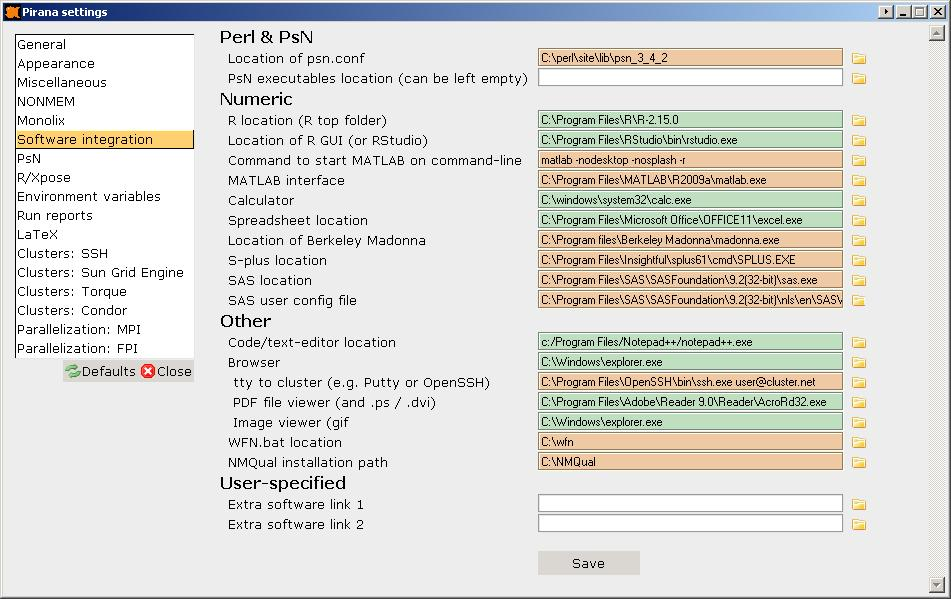
\includegraphics[scale=.4]{images/settings_2.jpg}
    \caption{Software integration window}
\end{figure}

\subsubsection*{PsN}
\begin{itemize}
\item Refer to PsN quick guide for detailed support on using PsN with Pirana.
\item This settings window specified default command line parameters for PsN.
\end{itemize}

%% Fig 3
\begin{figure}[h] \centering
    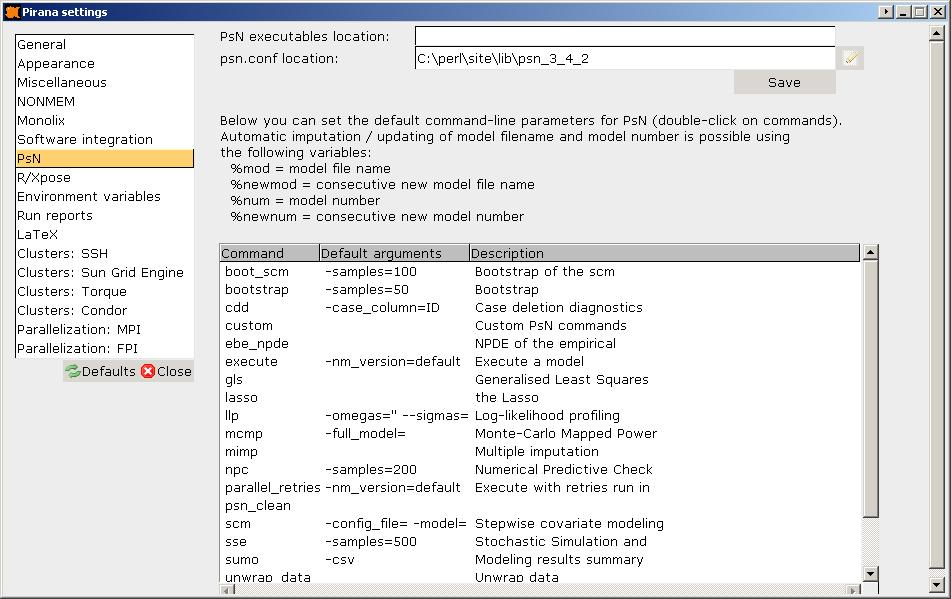
\includegraphics[scale=.4]{images/settings_3.jpg}
    \caption{PsN settings window}
\end{figure}

\subsubsection*{R/Xpose}
\begin{itemize}
\item \emph{Initialization commands} may be used to load specific R libraries when executing R/Xpose. 
\item \emph{PDF/PNG/GIF/EPS Arguments}: Default plotting arguments for R printing devices.
\item \emph{Sweave preamble/postamble}: If the Sweave functionality from Xpose is used, the default LaTeX pre/postable may be specified here.
\end{itemize}

%% Fig 4 
\begin{figure}[h] \centering
    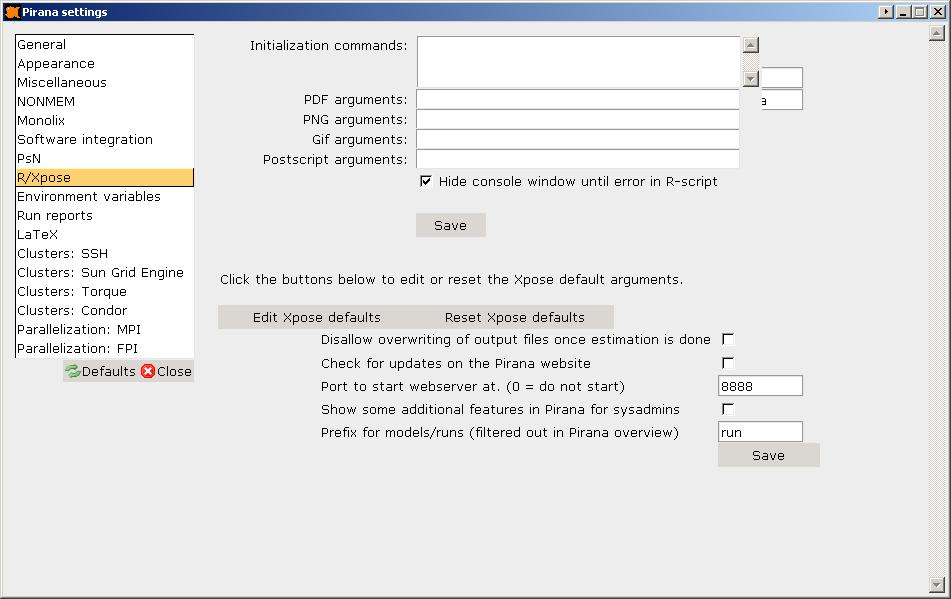
\includegraphics[scale=.4]{images/settings_4.jpg}
    \caption{R/Xpose settings window}
\end{figure}

\subsubsection*{Clusters}
\begin{itemize}
\item For more information on settings for clusters, please refer to the Clusters quick guide.
\end{itemize}

\subsubsection*{Configure the Sun Grid Engine}
\begin{itemize}
\item Defaults for working with SGE may be defined here.
\end{itemize}

%% Fig 5
\begin{figure}[h] \centering
    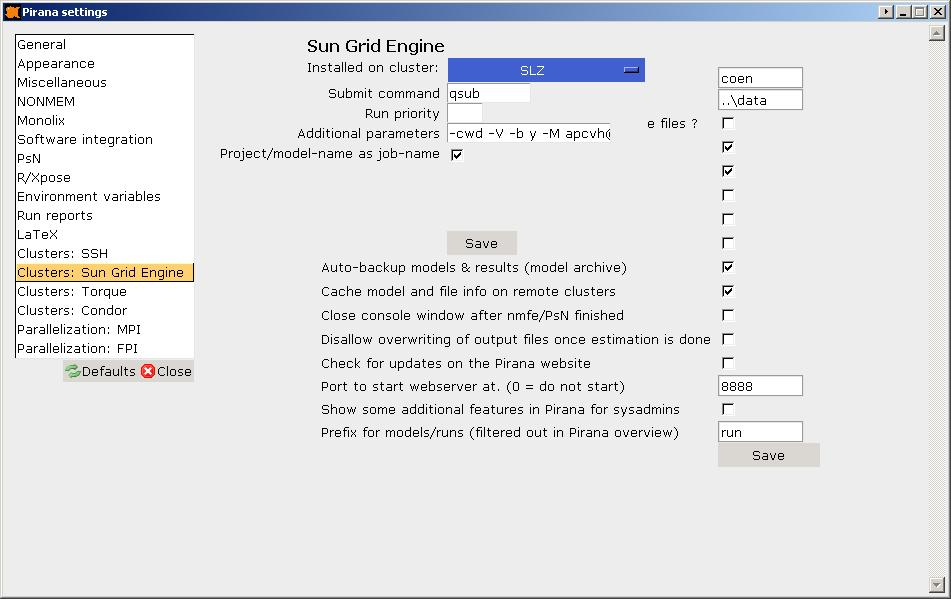
\includegraphics[scale=.4]{images/settings_5.jpg}
    \caption{SGE}
\end{figure}

\subsubsection*{Miscellaneous}
\begin{itemize}
\item \emph{File extensions}: File extensions are important to define because this wil determine if model files are shown (i.e. mod or ctl), and if NONMEM output files are correctly read (i.e. res or lst). 
\item \emph{Linux}: Refers to defaults for terminal and shell
\item \emph{PCluster}: Settings for working with PCluster (unsupported, refer to PCluster manual).
\item \emph{NMQual settings}: Here, folders may be added to PATH or LIBRARY\_PATH environmental variables.
\end{itemize}

%% Fig 6
\begin{figure}[h] \centering
    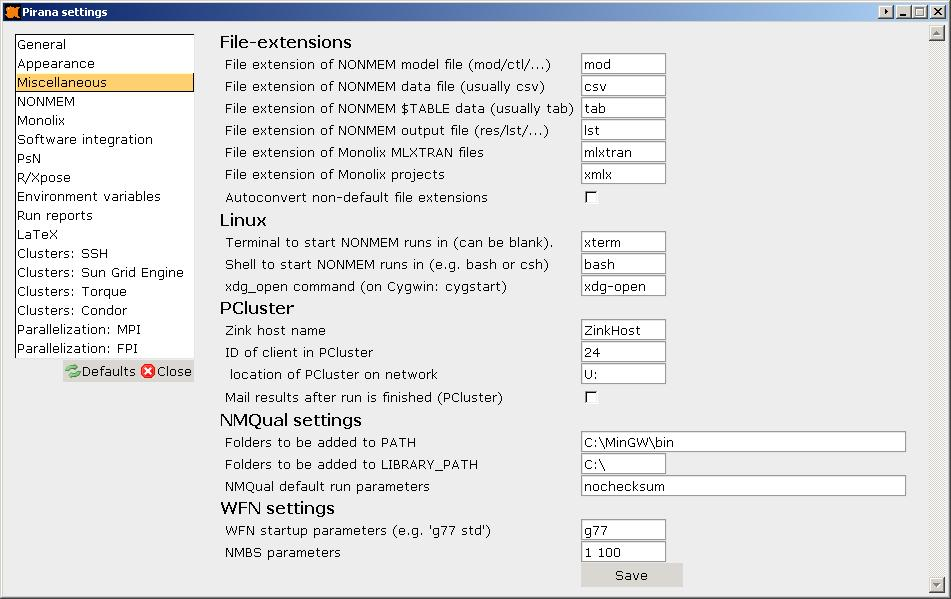
\includegraphics[scale=.4]{images/settings_6.jpg}
    \caption{Miscellaneuous settings}
\end{figure}

\clearpage
\section{Quick Guide: Setting up NONMEM in Pirana}
\begin{center}
   {\colorbox{grey2}{
         \begin{minipage}[t]{0.9\textwidth}
\subsubsection*{Scope}
This Pirana Quick Guide explains how add NONMEM (nmfe) installations
to Pirana. This procedure is not required for PsN installations, which
are automatically recognized if PsN is configured appropriately. It
will also be discussed how to set up installations that use Intel
Fortran v11 as compiler within Pirana. Note: in this quick guide it
will be assumed that you already have installed NONMEM.
          \end{minipage}
      }
   }
\end{center}

\subsubsection*{Add NONMEM installation setting window}
\begin{itemize}
\item Go to File $\rightarrow$ Settings $\rightarrow$ NONMEM. The
  dialog window shown in Figure 1 appears.
\item In this dialo, local (top part) and remote (bottom part) NONMEM
  installations may be defined.
\end{itemize}

\begin{figure}[h] \centering
    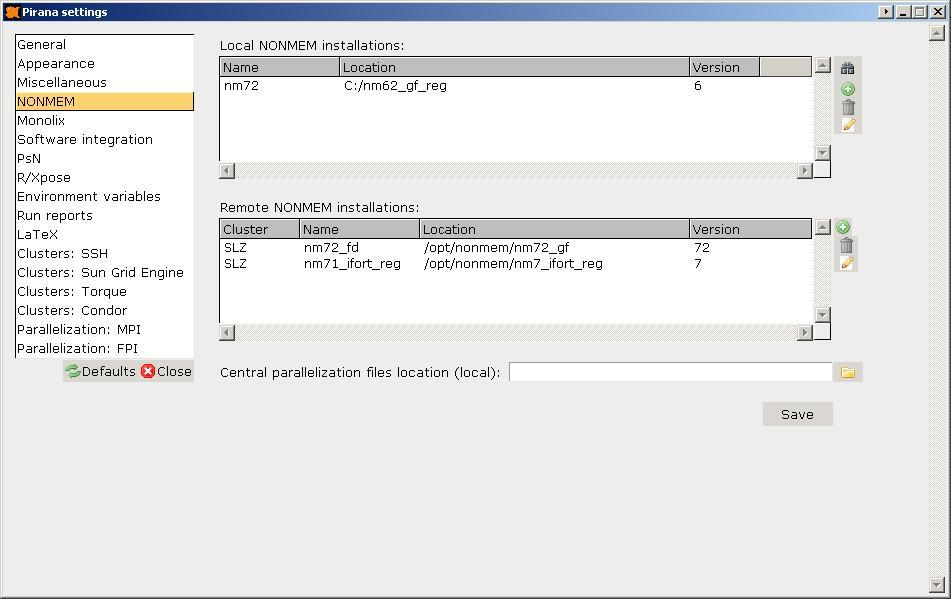
\includegraphics[scale=.42]{images/addnonmem_1.jpg}
    \caption{Adding a NONMEM installation\label{fig:Fig1}}
\end{figure}

\subsubsection*{Adding local nonmem installations }
\begin{itemize}
\item By pressing the Find icon (Figure \ref{fig:Fig1}, blue square), Pirana will
  automatically attempt to find any local NONMEM installations at
  common installation locations.
\item If you installed NONMEM at a non-standard location and Pirana is
  not able to find it automatically, you will have to add it manually, by
  pressing the \emph{\Large{+}} button (Figure \ref{fig:Fig1}, red square).
\item A window (Figure \ref{fig:Fig2}) will appear where the name and location of
  the NONMEM installation may be entered. The version of NONMEM will
  be automatically detected.
\item After adding NONMEM installations, please press the Save button (Figure
  \ref{fig:Fig1}). The local NONMEM installations will then be available in Pirana.
\end{itemize}

\begin{figure}[h] \centering
    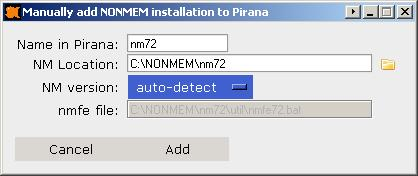
\includegraphics[scale=.5]{images/addnonmem_2.jpg}
    \caption{Adding a local NONMEM installation\label{fig:Fig2}}
\end{figure}

\subsubsection*{Adding remote nonmem installations }
\begin{itemize}
\item Auto-detection of NONMEM installations is not available for
  remote NONMEM installations, they will have to be added manually.
\item Press the \emph{\Large{+}} button next to \emph{Remote NONMEM}
  installations, to add a remote installation.
\item A window (Figure \ref{fig:Fig3}) appears, in which the installation name, the
  associated cluster, the location and the version can be defined.
\item After adding NONMEM installations, press the Save button (Figure
  \ref{fig:Fig1}). The remote NONMEM installations are now available in Pirana.
\end{itemize}

\begin{figure}[h] \centering
    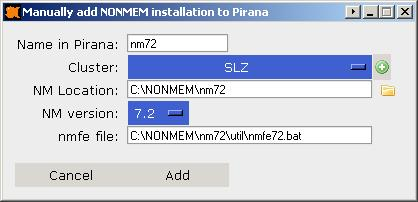
\includegraphics[scale=.5]{images/addnonmem_3.jpg}
    \caption{Adding a remote NONMEM installation\label{fig:Fig3}}
\end{figure}

\subsubsection*{Using Intel Fortran 11 for Windows together with NONMEM/PsN}
The Intel Fortran 11 compiler requires the user to set several
environmental variables. If these variables are correctly defined
system-wide, NONMEM installations using Intel Fortran should already
work. However, if you are not able to set the environment variables
system-wide, or you experience problems, you can also use Pirana to
set them for you.

\begin{itemize}
\item Please refer to posts on NMusers (such as
  \href{'http://www.cognigencorp.com/nonmem/current/2009-October/2077.html''}{this}
  one) where it is explained how environmental variables should be
  defined for Intel Fortran. These may differ slightly from system to
  system, so we can't give a fixed solution here. The common way in
  Windows to set these environment variables is by going to the
  Control panel $\rightarrow$ System settings $\rightarrow$
  Environment variables.  However, Pirana offers three alternative
  solutions to define the required environmental variables.
\item The first option is through Tools $\rightarrow$ NONMEM
  $\rightarrow$ Environmental variables. Setting the environment
  variables here will set them prior to executing a model (nmfe-only).
\item The second option is through File $\rightarrow$ Settings
  $\rightarrow$ Software integration $\rightarrow$ 'Add this to path
  at Pirana startup. Note that this only adds locations to the PATH
  environment variable. Most likely, you will have to set a few more
  environment variables as well.
\item The last option is by adding a text file add\_env.txt or
  set\_env.txt to the main Pirana folder. These text files can be used
  to \emph{add} to or \emph{set} any environmental variables. These
  files could for instance look as below.
\end{itemize}
   {\colorbox{grey2}{
         \begin{minipage}[t]{0.5\textwidth}
          {\ttfamily
   PATH=C:$\backslash$nmvi$\backslash$run;C:$\backslash$MinGW$\backslash$bin\\
   LIB=C:$\backslash$Program files$\backslash$Intel
   fortran$\backslash$bin
}
          \end{minipage}
      }
   }



\clearpage
\section{Quick Guide: Setting up cluster connections}
\begin{center}
   {\colorbox{grey2}{
         \begin{minipage}[t]{0.9\textwidth}
         \subsubsection*{Scope}
     This Pirana Quick Guide explains how to prepare,  configure and work with a cluster over SSH, 
and how to subsequently work with Pirana to execute models on the cluster. 
         \end{minipage}
      }
   }
\end{center}

\subsubsection*{Preparation: SSH access}
In order to execute runs on a cluster from a local system with Pirana, SSH access
to the cluster from your local computer must be available. 
\begin{itemize}
\item For Windows, the easiest way to do this is to install
  \href{'http://www.chiark.greenend.org.uk/~sgtatham/putty/''}{Putty}. Make
  sure that you install the complete version of PuTTY, including the
  command line tool \emph{plink.exe}.
\item After installation, make sure Putty is available in the system
  path, or add the location of the Putty folder to the internal Pirana
  path via File $\rightarrow$ Settings $\rightarrow$ Software
  integration $\rightarrow$ 'Add this folder(s) to PATH at Pirana
  startup'.
\item On Linux and Mac OSX, ssh is most likely already installed.
\end{itemize}

\subsubsection*{Preparation: Mounting a cluster folder as local drive}
A remote folder on the cluster should be mounted as a local drive
letter (e.g. R:) on your system. There are several ways to do this,
some of which are described below. Please check with your system
administrator if you don't manage to mount the cluster as a local drive.
\begin{itemize}
\item If the cluster is running Samba, a drive letter may be mounted
  through My Computer $\rightarrow$ Extra $\rightarrow$ Network
  connections.
\item If only SSH (SFTP) access is available, software such as
  \href{'http://www.expandrive.com/''}{Expandrive} may be considered.
\end{itemize}



\subsubsection*{Configuring the cluster}
If the remote cluster folder can be mounted as drive letter on your
system, and you have installed putty, cluster access may now be
configured in Pirana.
\begin{itemize}
\item Access the settings menu via File $\rightarrow$ Settings
  $\rightarrow$ Clusters. A screen is obtained as depicted in Figure  \ref{fig:Fig1}.

\begin{figure}[h] \centering
    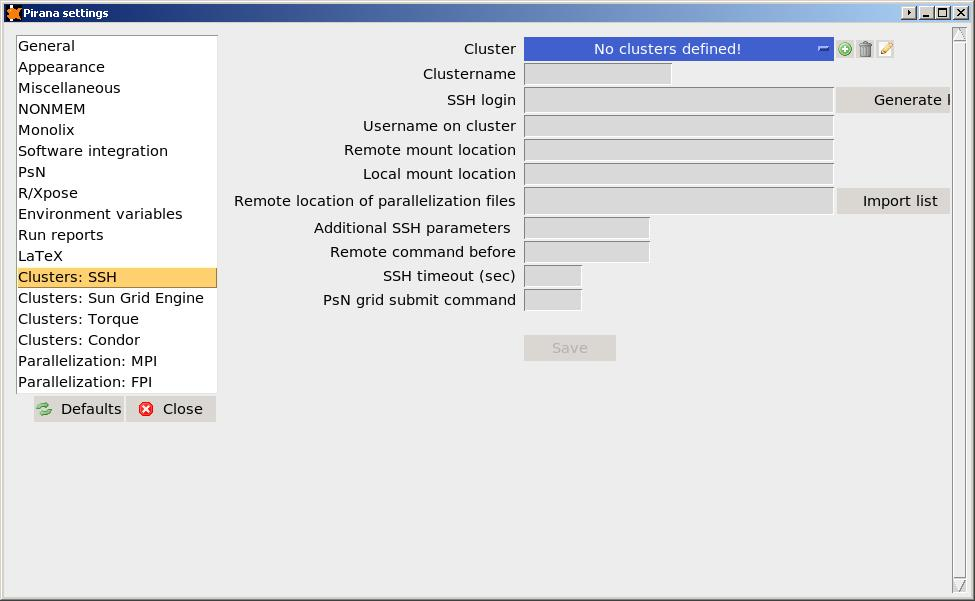
\includegraphics[scale=.4]{images/cluster_1.JPG}
    \caption{Cluster settings window\label{fig:Fig1}
}
\end{figure}

\item Select the \emph{\Large{+}} sign to add a new cluster. Some
  initial settings are pre-entered in the textboxes of the newly
  defined cluster (Figure  \ref{fig:Fig2}), but these have to be updated to match
  your cluster.

\begin{figure}[h] \centering
    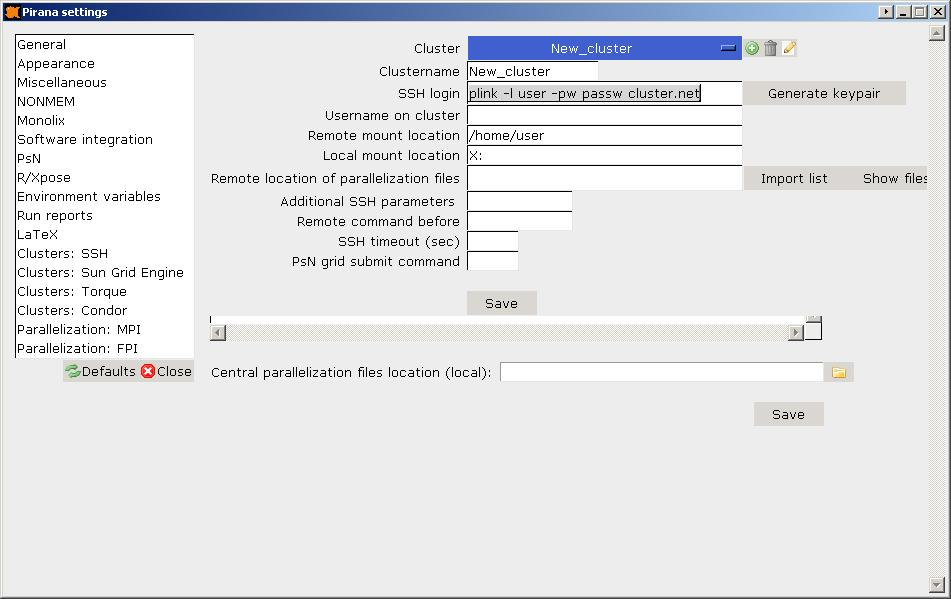
\includegraphics[scale=.4]{images/cluster_2.JPG}
    \caption{Pre-entered text after adding a new cluster\label{fig:Fig2}
}
\end{figure}

\item In the textbox \emph{Clustername}, define a name for the cluster
  (can be anything).
\item The textbox \emph{SSH login} should contain the command to
  connect to the cluster. If Putty is used, this command will start
  with \emph{plink}, followed by the user name, password and name or
  IP address of the cluster access node, e.g. 'plink -l myname -p
  mypassw pkpd.server.org'. Passwordless access using a RSA key is
  also possible.
\item The textbox \emph{Remote mount location} refers to a folder on
  the cluster which you have mounted as local drive.
\item The textbox \emph{Local mount location} should contain the
  drive-letter on the local system which corresponds with the remote
  cluster path defined in the previous textbox.
\item In the following textboxes, \emph{Additional SSH parameters},
  and \emph{Remote commands before} connecting to the cluster, and the
  \emph{PsN grid submit command} may be defined, but these are not
  required.
\item  An example of a fully configured cluster is depicted in Figure  \ref{fig:Fig3}.
\end{itemize}

\begin{figure}[h] \centering
    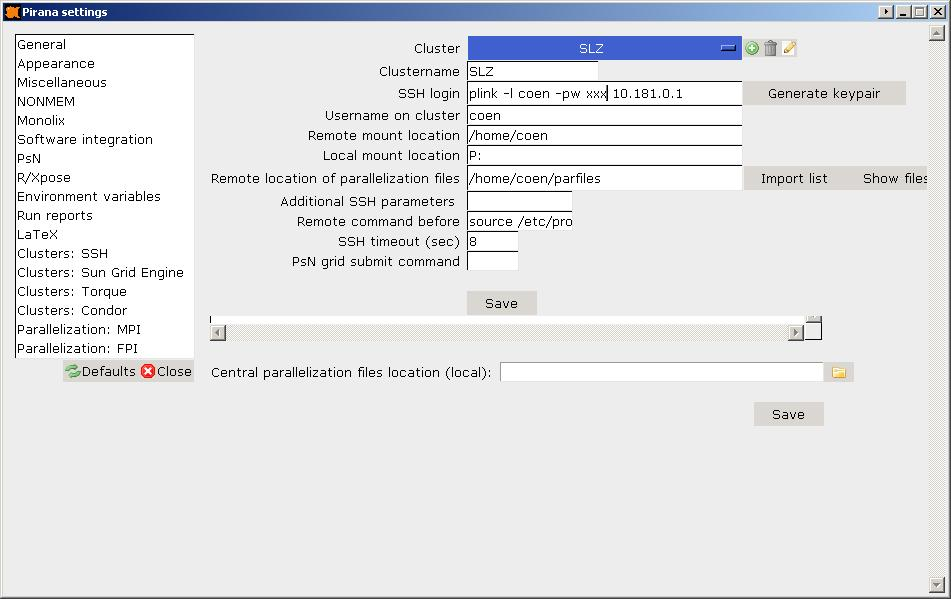
\includegraphics[scale=.4]{images/cluster_3b.JPG}
    \caption{Settings of a fully configured cluster\label{fig:Fig3}
}
\end{figure}

\subsubsection*{Working with the cluster}

  \begin{itemize}
  \item Any runs which are to be submitted to the cluster should be in
    a location on the drive which you specified the remote cluster
    mount location.
  \item A model can be run on the cluster via either \emph{nmfe} or
    \emph{PsN}, which are described separately below.
\end{itemize}

\subsubsection*{Submitting a run to the cluster via nmfe}
  \begin{itemize}
  \item When submitting a run via nmfe, after selecting a model and
    opening the 'nmfe'-run dialog, select a cluster to connect to
    (Figure  \ref{fig:Fig4}, blue quare).
  \item The option \emph{Submit to [..]} should be selected if the run is to be
    submitted to a job scheduler. (Figure  \ref{fig:Fig4}, green square). 
    Currently supported schedulers are Sun Grid Engine (SGE), Torque and Condor.
  \item Optionally, for NONMEM 7.2, parallalization files may be
    selected.
  \item Start the run.
\end{itemize}

\begin{figure}[h] \centering
    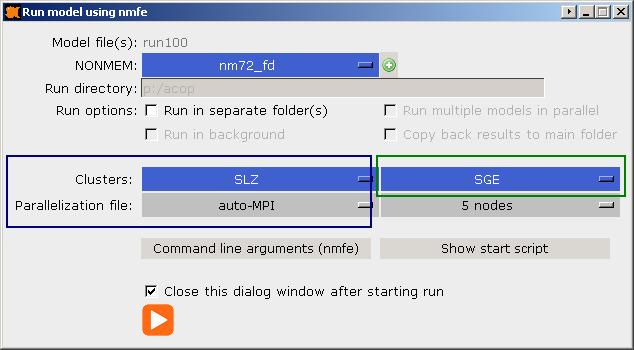
\includegraphics[scale=.4]{images/cluster_4.JPG}
    \caption{Defining cluster settings for a nmfe run\label{fig:Fig4}
}
\end{figure}

\pagebreak

\subsubsection*{Submitting a run to the cluster via PsN}
  \begin{itemize}
  \item Select a cluster for the PsN run (Figure 5, orange square).
  \item Add optional arguments to the PsN argument, such as
    \emph{-run\_on\_sge}, if the run is submitted to SGE (Figure  \ref{fig:Fig5},
    red square).
  \item Several PsN arguments are available for other job schedulers
    such as LSF (Figure  \ref{fig:Fig5}, blue square). Please note that
    the configuration of these job schedulers should be done in the
    psn.conf file on the cluster. Please refer to the PsN manual for
    more information about this.
  \item Start the run.
\end{itemize}

\begin{figure}[h] \centering
    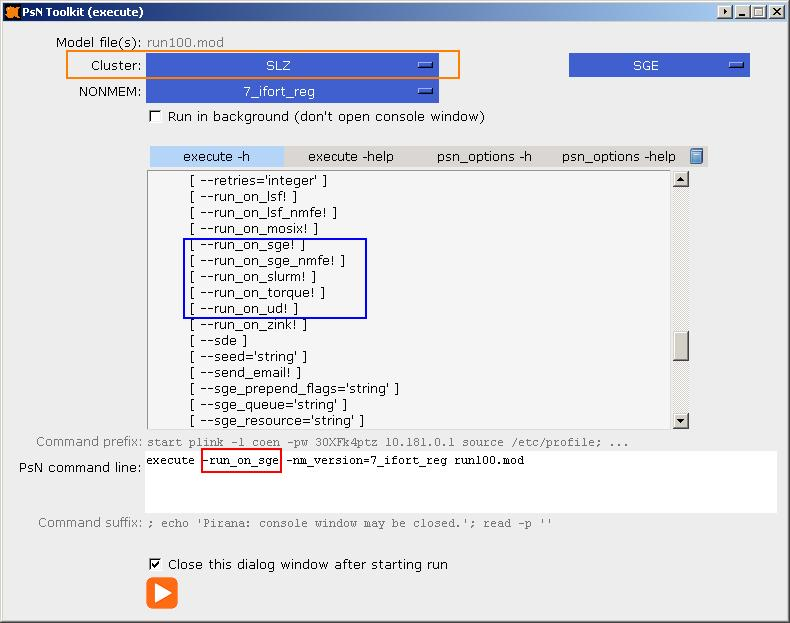
\includegraphics[scale=.4]{images/cluster_5.JPG}
    \caption{Defining cluster settings for a PsN run\label{fig:Fig5}
}
\end{figure}

\subsubsection*{Monitoring jobs on a SGE cluster}
  \begin{itemize}
  \item If SGE, Torque or Condor is used as job managment system, the queue may be
    monitored using the integrated monitor in Pirana.
  \item This feature may be accessed by clicking the SGE icon in the
    main Pirana interface (Figure \ref{fig:Fig2}, red square).
  \item In the interface that is opened, an overview will be presented
    of the jobs that are currently running, scheduled, or have
    recently been finished. Some information about available nodes in
    the SGE cluster can also be viewed.
  \item By right-clicking on a job, you can view more information
    about it, or kill it. Please note that not only NONMEM jobs are
    shown here, but any compute job (e.g. MATLAB).
\end{itemize}

\begin{figure}[h] \centering
    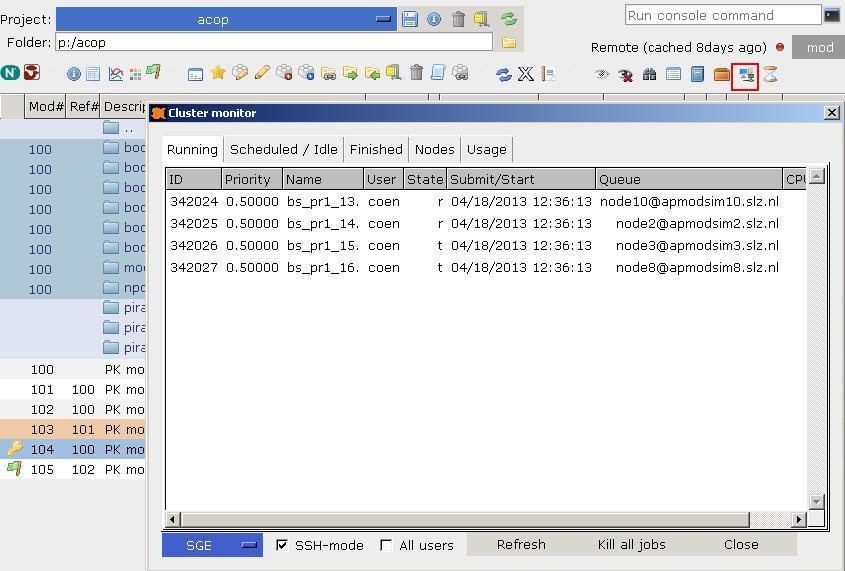
\includegraphics[scale=.4]{images/cluster_6.JPG}
    \caption{Cluster run window\label{fig:Fig6}
}
\end{figure}


\clearpage
\section{Quick Guide: Working with models}

\subsubsection*{Introduction}
\begin{itemize}
\item All models and their associated results available in a folder in
  Pirana are depicted in the main Window.
\item When selecting a model and using the right mouse-button menu, a
  range of actions may be performed on the selected model.
\item Most manipulations (duplicating, removing, etc.) of models are
  available via the sub-menu \emph{Actions} (Figure \ref{fig:Fig1}).
\end{itemize}

%% Fig 1
\begin{figure}[h] \centering
    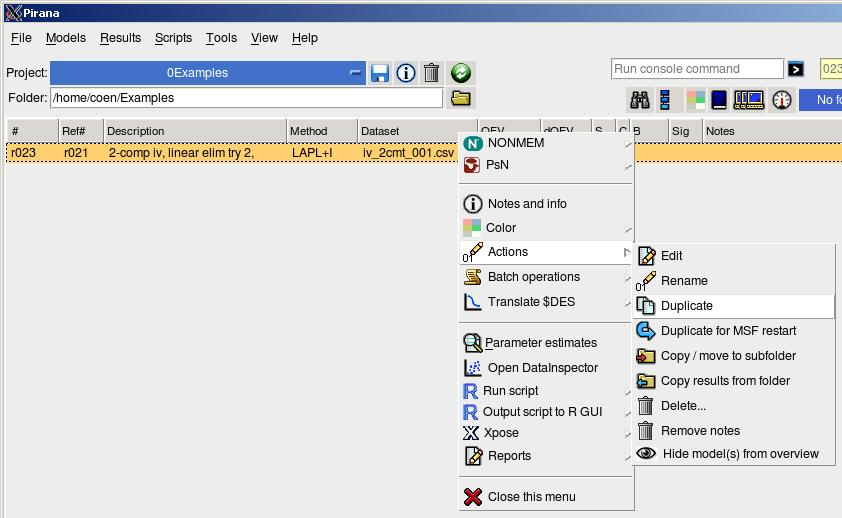
\includegraphics[scale=.4]{images/working_3.jpg}
    \caption{Pirana window with context menu\label{fig:Fig1}}
\end{figure}

%%%%%%%%%%%%%%%%%%%

\subsubsection*{Running a model}
\begin{itemize}
\item Select the model and open the right-mouse button context menu.
\item Select the preferred methode of running the model, i.e. NONMEM $
  \rightarrow$ nmfe, or PsN $ \rightarrow$ execute. 
\item If you are using nmfe to run a model, NONMEM has to be
  registered within Pirana first (refer to the Quick Guide on
  installing NONMEM). If PsN is installed, Pirana will automatically
  recognize this.
\end{itemize}

%%%%%%%%%%%%%%%%%%%

\subsubsection*{Running a model using nmfe} 
After having selected Run via nmfe, the Run window depicted in Figure
\ref{fig:Fig2} will appear. A number of options are available here, before
executing the run.
\begin{itemize}
\item \emph{NONMEM}: The preferred NONMEM installations may be selected. 
\item \emph{Run in seperate folder(s)}: A NONMEM run may be executing
  in a sub-folder, to enable to run multiple runs
  simultaneously. Results from a subfolder can be imported to the main
  folder in Pirana.
\item \emph{Run in background}: No console window is opened, the model
  is run in the background.
\item \emph{Clusters-Submit to SGE}: Run on a cluster using SGE (optional). 
\item \emph{Clusters-Parallelization}: Run using parallelization
  available in NONMEM 7.2 (optional).
\item \emph{Connect to}: Cluster (optional). Connect to a
  cluster. Please refer to the Quick Guide on Clusters for more information.
\item \emph{Script contents}: The script which is executed to run the model.
\item The run may be executed using the \emph{\Large{$>$}} button.
\end{itemize}

%% Fig 2
\begin{figure}[h] \centering
    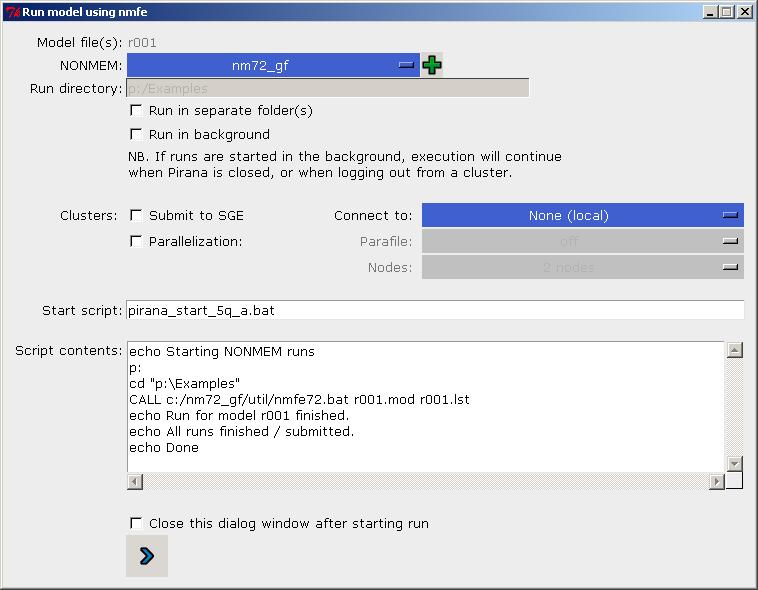
\includegraphics[scale=.4]{images/working_4.jpg}
    \caption{Run window for nmfe\label{fig:Fig2}}
\end{figure}

%%%%%%%%%%%%%%%%%%%

\subsubsection*{Running a model using PsN} 
After having selected Run via PsN, the PsN run window depicted in
Figure \ref{fig:Fig3} will appear. Again, a number of options are available here,
before executing the run.
\begin{itemize}
\item \emph{Cluster}: Cluster to connect to (optional). Please refer
  to the Quick Guide on Clusters for more information.
\item \emph{NONMEM}: The preferred NONMEM installations may be
  selected. 
\item \emph{Run in background}: After executing the model, output is
  not printed to the screen.
\item \emph{PsN command line}: This is the command line which is
  executed. Additional PsN arguments may be added here.
\item The top part of the window shows an overview for of available
  PsN arguments.
\end{itemize}

%% Fig 3
\begin{figure}[h] \centering
    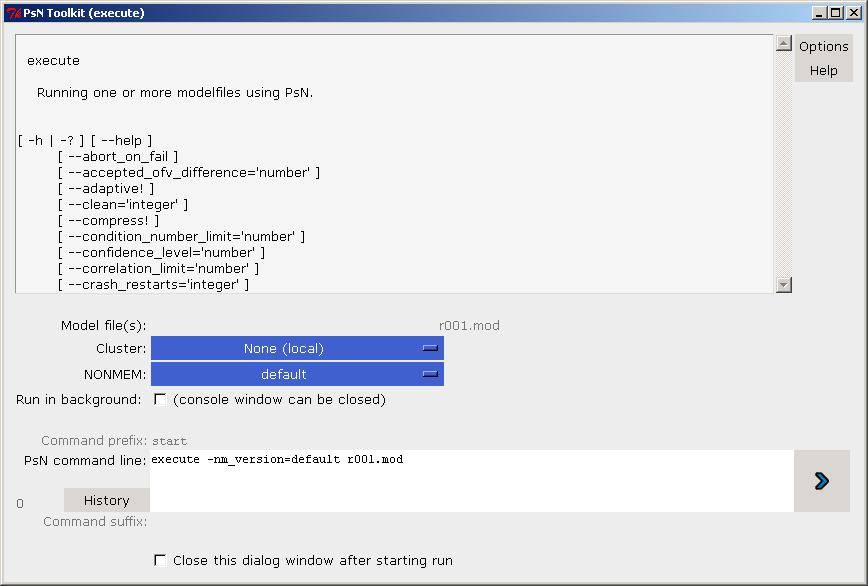
\includegraphics[scale=.4]{images/working_5.jpg}
    \caption{Run window for PsN\label{fig:Fig3}}
\end{figure}

%%%%%%%%%%%%%%%%%%%

\subsubsection*{Generating an empty control stream}
\begin{itemize}
\item An empty control stream may be generated via  Models $ \rightarrow$  New model (Figure \ref{fig:Fig4}).
\item Choose the template control stream that you want to use.
\item The control stream will be opened in the text editor defined in Settings.
\end{itemize}

%% Fig 4
\begin{figure}[h] \centering
    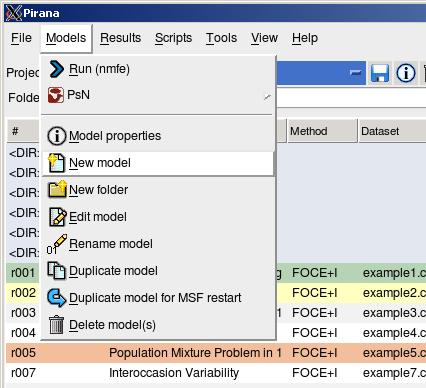
\includegraphics[scale=.5]{images/working_1.jpg}
    \caption{Create an empty model\label{fig:Fig4}}
\end{figure}

\subsubsection*{Generating a new control stream using the Wizard}
\begin{itemize}
\item Empty, partly pre-coded PK models may be generated using the Wizard (Tools $ \rightarrow$ Wizards). 
\item In the Wizards menu (Figure \ref{fig:Fig5}), select PK NONMEM model. 
\item After finishing the Wizard, a new control stream will be created and opened in the editor.
\end{itemize}

%% Fig 5
\begin{figure}[h] \centering
    \includegraphics[scale=.5]{images/working_2.jpg}
    \caption{Create a new model using the Wizard\label{fig:Fig5}}
\end{figure}

\subsubsection*{Editing  a control stream}
\begin{itemize}
\item A control stream visible in the main Pirana window may be edited by double clicking on the model.
\item Alternatively, this may be done through the right-mouse button menu Actions $ \rightarrow$ Edit.
\item Please note that an alternative code editor can be defined
  through File $ \rightarrow$ Settings $ \rightarrow$ Software
  integration. The default in Pirana is notepad.exe, but it is highly
  recommended to change this to an appropriate code editor such as
  Emacs, ConText, or PSPad.
\end{itemize}

\subsubsection*{Duplicating a control stream}
\begin{itemize}
\item A control stream may be duplicated through the right-mouse
  button menu Actions $ \rightarrow$ Duplicate (Figure \ref{fig:Fig1}).
\item In the resulting Duplication window (Figure \ref{fig:Fig6}), you can choose
  to update parameter estimates in the new file to the ones estimated
  for the current model, fix the parameter estimates, change the
  file numbers in \$TABLE and \$EST records.
\item Please note that to correctly duplicate with updated parameter
  estimates, you are required to adhere to some coding guidelines,
  especially for the \$OMEGA and \$SIGMA blocks. See the Pirana manual
  for more information.
\item After pressing the Duplicate button, a new model will be created
  and opened in the editor.
\end{itemize}

%% Fig 6
\begin{figure}[h] \centering
    \includegraphics[scale=.5]{images/working_6.jpg}
    \caption{Create a new model using the Wizard\label{fig:Fig6}}
\end{figure}

\subsubsection*{Renaming a control stream}
\begin{itemize}
\item A control stream may be renamed through the right-mouse
  button menu Actions $\rightarrow$ Rename (Figure \ref{fig:Fig1}). Some of the
  same options as under duplication are available.
\end{itemize}

\subsubsection*{Deleting a control stream}
\begin{itemize}
\item A control stream may be deleted by selecting the right-mouse
  button menu Actions $\rightarrow$ Delete (Figure \ref{fig:Fig1}). Alternatively,
  a can be selected and subsequently the keyboard button DELETE can be
  pressed.
\item In the dialog that is opened, you can select what to delete:
  only the control stream (models), or also the associated results
  files, datasets. If you have selected one or more folders in the
  main overview to be deleted, the 'folder' option should be checked to
  actually delete these as well.
\end{itemize}

\subsubsection*{Viewing parameter estimates inside the GUI}

\begin{itemize}
\item During model building, parameter estimates can be viewed by selecting a run, and opening the Estimates Tab on the right panel (Figure \ref{fig:Fig7}).
\item The parameter estimates window can be opened from the option Parameter estimates in the context menu (right mouse button) (Figure \ref{fig:Fig8}), or alternatively from the button in the right panel with estimates. 
\item Results from the table can be exported to CSV, LaTeX or HTML, and different transformations of variances can be selected.
\item When selecting multiple runs, parameter estimates can be compared with each other (Figure \ref{fig:Fig9}). 
\end{itemize}

\begin{figure}[h] \centering
    \includegraphics[scale=.25]{images/report_1.png}
    \caption{Viewing estimates in right panel in the Pirana GUI\label{fig:Fig7}}
\end{figure}

\begin{figure}[h] \centering
    \includegraphics[scale=.35]{images/report_2.png}
    \caption{Parameter estimates window\label{fig:Fig8}}
\end{figure}

\begin{figure}[h] \centering
    \includegraphics[scale=.35]{images/report_4.png}
    \caption{Parameter estimates comparison\label{fig:Fig9}}
\end{figure}



\clearpage
\section{Quick Guide: Creating reports}

\begin{center}
   {\colorbox{grey2}{
         \begin{minipage}[t]{0.9\textwidth}
\subsubsection*{Scope}
This Pirana Quick Guide aims to provide an overview of current reporting functionality
available in Pirana.
          \end{minipage}
      }
   }
\end{center}


\subsubsection*{Overview of functionality}
The following functionality for reporting is available in Pirana:
\begin{itemize}
\item Run reports in various formats (HTML, Word, text, LaTeX, 
 pdfLaTeX)
\item Run records of multiple runs (CSV/Excel, HTML, Word, text)
\item Visual interactive run records.
\item Execution log files of executed runs.
\end{itemize}



\subsubsection*{Generating run reports}
\begin{itemize}
\item From the menu or context menu, the option Reports can be accessed, which allows generation of various run reports (Figure \ref{fig:Fig4}) of one or more runs (if more runs are selected simultaneously).
\item The components to be included in the report can be modified (Reports menu, option "Include in reports")
\item Generated run reports are placed into a pirana\_reports folder, and can be accessed from the tab Reports in the right panel of Pirana (Figure \ref{fig:Fig5}). 
\end{itemize}

\begin{figure}[h] \centering
    \includegraphics[scale=.4]{images/report_5.png}
    \caption{HTML report\label{fig:Fig4}}
\end{figure}

\begin{figure}[h] \centering
    \includegraphics[scale=.25]{images/report_3.png}
    \caption{Overview of available reports in right panel\label{fig:Fig5}}
\end{figure}

\subsubsection*{Generating run records}
\begin{itemize}
\item Run records are documents that contain reports (e.g. as above) for all runs in the project folder.
\item Run records can be created under Results $\rightarrow$ Run records. 
\item The CSV run record is a CSV file that can be opened in excel containing a table of all results (e.g. description, OFV, estimates, RSEs etc) for each model. 
\end{itemize}


\subsubsection*{Generating a visual run record}
\begin{itemize}
\item The visual run record (VRR) is a SVG file which contains an
 interactive tree view of the model development process (Figure \ref{fig:Fig6}. 
\item Models are related to each other based on Pirana's reference model
 tags in the model file.
\item The visual run record can be created under Results $\rightarrow$. 
\end{itemize}

\begin{figure}[h] \centering
    \includegraphics[scale=.4]{images/vrr.png}
    \caption{Visual run record\label{fig:Fig6}}
\end{figure}





\clearpage
\section{Quick Guide: Graphical output in R}
\begin{center}
   {\colorbox{grey2}{
         \begin{minipage}[t]{0.9\textwidth}
\subsubsection*{Scope}
This Pirana Quick Guide explains how to use Pirana to generate and
modify diagnostic graphs using the integrated R scripts library.
          \end{minipage}
      }
   }
\end{center}

\vspace{10pt}

Pirana has an integrated library of R scripts which can be used to
generate diagnostic plots based on model output files. The library of
R scripts can also be easily edited or extended with new scripts.

\subsubsection*{Creating diagnostic plots}
\begin{itemize}
\item Select the model for which you want to create plots.
\item In the right panel under Scripts, select the desired script.
\item Via the context menu, select run script. 
  clicking the right mouse button, and then selecting 'Run script',
  and subsequently selecting the plot you want to create (Figure \ref{fig:Fig1}).
\item The plot will be created and openened automatically (Figure \ref{fig:Fig2}).
 
\end{itemize}


\begin{figure}[hctb] \centering
    \includegraphics[scale=.3]{images/graphs_1.jpg}
    \caption{Running a script on a model run\label{fig:Fig1}}
\end{figure}

\begin{figure}[h] \centering
    \includegraphics[scale=.45]{images/graphs_3.jpg}
    \caption{Diagnostic plot created\label{fig:Fig2}}
\end{figure}


\subsubsection*{Troubleshooting problems with plot creation}
\begin{itemize}
\item If an error occurs, the R output will be displayed, which can be
used to diagnose the error (Figure \ref{fig:Fig3}). 
\item Most frequently this is due to a variable missing in the output table 
files (e.g. column IPRED not available in output table).
\item The expected input variables for each script are depicted at the bottom of 
the right panel. 
\end{itemize}

\begin{figure}[hctb] \centering
    \includegraphics[scale=.45]{images/graphs_2.jpg}
    \caption{Output of the script\label{fig:Fig3}}
\end{figure}


\subsubsection*{Customizing diagnostic plots}
\begin{itemize}
\item Instead of running the script through Run Script (above), the
  script may also be outputted to the R GUI ("Output script to R GUI")
  (Figure \ref{fig:Fig4}). Now, you can easily tweak the plot, and save it in the
  format you like. 
\item Afrter sending the script to R GUI, it will be opened there,
  where it may be further modified. Next, the script can be executed
  and the plot will be created within the R GUI (Figure 5).
\end{itemize}

\begin{figure}[h] \centering
    \includegraphics[scale=.3]{images/graphs_4.jpg}
    \caption{Output of a script to the R GUI for further customization\label{fig:Fig4}}
\end{figure}


\subsubsection*{Editing and creating scripts}
\begin{itemize}
\item When one whishes to permanently make changes to the scripts
  library, this can be done using the option "Edit script" in the right panel context menu.
  (Figure \ref{fig:Fig6}).
\item Any changes made to the script will be saved permanently. You
  can choose to make changes in the script that are originally
  supplied with Pirana, or have them in your own user library.
\item Script files are located either in the user folder
  (e.g. C:$\backslash$Documents and
  Settings$\backslash$Username
$\backslash$.pirana$\backslash$scripts), or in the
  main Pirana folder (e.g. C:$\backslash$Program
  Files$\backslash$Pirana). The organization of scripts in sub-menus
  is according to the folder structure in these scripts folders
  (Figure \ref{fig:Fig7}), and can be adjusted accordingly.
\item Note that when you install a new version of Pirana over the old
  one, any R script you have in the Pirana folder will be overwritten
  with the one supplied by the new version of Pirana (if you haven't
  given the R-script another name).
\item Through the menu 'Scripts' $\rightarrow$ 'New scripts', it is
  also possible to define new scripts. Please note that at current,
  you will have to restart Pirana for the script to show up in the
  interface.
\end{itemize}

\begin{figure}[h] \centering
    \includegraphics[scale=.3]{images/graphs_6.jpg}
    \caption{Editing templates for scripts\label{fig:Fig6}}
\end{figure}

\begin{figure}[h] \centering
    \includegraphics[scale=.5]{images/graphs_7.jpg}
    \caption{Script files present in the scripts sub-folder of Pirana\label{fig:Fig7}}
\end{figure}



\clearpage
\section{Quick Guide: Creating a VPC}

\begin{center}
   {\colorbox{grey2}{
         \begin{minipage}[t]{0.9\textwidth}
\subsubsection*{Scope}
This Pirana Quick Guide explains how to use Pirana to generate VPC
data using PsN, and how to subsequently use that data to create VPC plots
with Xpose using different plotting options. 
          \end{minipage}
      }
   }
\end{center}

\subsubsection*{Generating data for the VPC}
\begin{itemize}
\item Select the model for which a VPC should be created, and select
  the option VPC via the menu below your right-mouse button (PsN $
  \rightarrow$ Model evaluation $ \rightarrow$ vpc) (Figure \ref{fig:Fig1}).
\end{itemize}

\begin{figure}[h] \centering
    \includegraphics[scale=.4]{images/vpc_1.jpg}
    \caption{Selecting a run and executing the PsN/VPC Toolkit run window
     \label{fig:Fig1}}
\end{figure}

\begin{itemize}
\item In the resulting PsN settings window, the command for running
  creating the vpc can be specified (Figure \ref{fig:Fig2}). The vpc command takes
  many arguments which alters the way the vpc is calculated, e.g. you
  can specify stratifications, binning, dependent variable etc.
\item Arguments may be added in the text box at the lower part of the
  PsN run window (orange square). Make sure to separate the arguments
  by a space, and start each argument with a `-'.
\item A full overview of possible arguments and their use may be
  viewed in the upper part of the PsN run window. By clicking on
  `Help', additional help on these arguments is available (small blue square).
\item When all arguments for the VPC dataset have been defined
  correctly, the PsN/vpc run may be executed (green square).
\end{itemize}

\begin{figure}[h] \centering
    \includegraphics[scale=.4]{images/vpc_2.jpg}
    \caption{PsN/vpc Toolkit run window
     \label{fig:Fig2}}
\end{figure}

\begin{itemize}
\item If the VPC run is not executed in the background, a run window
  will appear similiar to Figure Figure \ref{fig:Fig3}. Make sure to check if no errors
  are reported in this step. If the vpc finishes correctly, it will
  report something like `Done reading and formatting data, finishing run.'
\end{itemize}

\begin{figure}[h] \centering
    \includegraphics[scale=.5]{images/vpc_3.jpg}
    \caption{Output after execution of VPC run using PsN
    \label{fig:Fig3}}
\end{figure}

\subsubsection*{Plotting the VPC data}

\begin{itemize}
\item If the VPC was run succesfull, a new folder will be created
  which is named npc\_dirX, at least if you did not specify another
  folder name manually (Figure \ref{fig:Fig3}, blue square).
\item If you don't see the folder yet in Pirana, press the folder
  refresh button (round green/white button). Also make sure that the folder filter is set to
  \emph{PsN folders} or \emph{All folders} (Figure \ref{fig:Fig3}, orange square).
\item Note that if you run the vpc command multiple times, multiple
  \emph{npc\_dir} folders will be created. It is therefore advisable
  to use the `-dir' option in PsN to specify a specific folder each
  time you run a vpc.
\end{itemize}

\begin{figure}[h] \centering
    \includegraphics[scale=.35]{images/vpc_4.jpg}
    \caption{VPC run folder created after execution of VPC run
    \label{fig:Fig4}}
\end{figure}

\begin{itemize}
\item Select the model for which the VPC was executed. (Figure \ref{fig:Fig5}).
\item Select Xpose $\rightarrow$ Run Xpose commands. This will open up
  the Pirana Xpose interface.
\end{itemize}

\begin{figure}[h] \centering
    \includegraphics[scale=.4]{images/vpc_5.jpg}
    \caption{Starting the 'Run Xpose commands' window on selected run.
    \label{fig:Fig5}}
\end{figure}

\begin{itemize}
\item Enter or select xpose.VPC in the command text field (Figure \ref{fig:Fig6},
  blue square). If any other commands are present in the list, remove these.
\item Next, arguments for the Xpose.VPC may be added (Figure \ref{fig:Fig6}, orange
  square).  The xpose.VPC help files may be accessed using the help
  button.
\item Several options are available for the output format. The easiest
  option is to automatically generate the graph and save as PDF
  (default) or PNG file (Figure \ref{fig:Fig6}, red square).
\item Alternative output formats are to generate the R-code only and
  open it in your R interface, or to to generate Sweave code for LaTeX
  documents.
\item If all settings have been configured, the VPC may be generated
  by pressing the execute button (Figure \ref{fig:Fig6}, green square).
\item If output was directed to a PDF or PNG file, this file will be 
  automatically opened by the PDF viewer you specified in Pirana's
  settings. (Figure \ref{fig:Fig7}). If you choose to generate R or LaTeX code,
  Pirana will open the R GUI or your code editor, and you will have to
  run the generated code manually.
\end{itemize}

\subsubsection*{Tweaking the VPC plot}
These VPCs may be further optimized by adjusting the many Xpose
arguments. Please check out the xpose VPC help files (which may be
accessed from the Run Xpose command window, or go the the Xpose
website for more information).

\begin{figure}[h] \centering
    \includegraphics[scale=.4]{images/vpc_6.jpg}
    \caption{The 'Run Xpose commands' window to generate the VPC graph
      \label{fig:Fig6}}
\end{figure}

\begin{figure}[h] \centering
    \includegraphics[scale=.4]{images/vpc_7.jpg}
    \caption{VPC obtained through PsN and Xpose
      \label{fig:Fig7}}
\end{figure}


\clearpage
\section{Quick Guide: Using Xpose from Pirana }
\begin{center}
   {\colorbox{grey2}{
         \begin{minipage}[t]{0.9\textwidth}
\subsubsection*{Scope}
This Pirana Quick Guide explains how to use Pirana to generate
diagnostic graphs using Xpose. Please note that a separate Quick Guide
describes how to create VPCs in PsN / Xpose.
          \end{minipage}
      }
   }
\end{center}

\subsubsection*{Generating appropriate NONMEM output tables for Xpose}
\begin{itemize}
\item Before Xpose diagnostic graphics can be generated, the model
  first needs to be executed while generating output tables in a
  specific format and naming.
\item Briefly, for a controlstream named run10.mod, output tables such
  as sdtab10 (observations/predictions), patab10 (parameters), cotab10
  (continuous covariates), and catab10 (categorical covariates) should
  be generated, with the NOPRINT and ONEHEADER options.
\item For more information on how to generate Xpose-ready \$TABLE
  output files, please refer to
  \href{'http://xpose.sourceforge.net/manual.pdf''}{the Xpose manual}.
\end{itemize}

\subsubsection*{Generating Xpose graphs using the integrated Pirana menu}
\begin{itemize}
\item Select the preferred run and select Xpose from the right
  mouse-button menu, and subsequently 'Run Xpose commands' (Figure
  \ref{fig:Fig1}).
\begin{figure}[h] \centering
    \includegraphics[scale=.32]{images/xpose_1.JPG}
    \caption{Selecting a run and executing the Rub Xpose commands winow\label{fig:Fig1}}
\end{figure}
\item In the dialog window that is opened, different Xpose graphs may
  be selected and defined (Figure \ref{fig:Fig2}).
\begin{figure}[h] \centering
    \includegraphics[scale=.45]{images/xpose_2.jpg}
    \caption{Run Xpose commands window\label{fig:Fig2}}
\end{figure}
\item From the \emph{Commands menu} (red square), \emph{multiple}
  Xpose plots may be added to the included list of Xpose plots.
\item Additional \emph{Arguments} may be specified for each Xpose
  command. A reference to possible arguments is provided under the
  \emph{\Large{?}} sign.
\item Several options are available for the output format of the
  \emph{Plots}. The easiest option is to automatically generate the
  graph and save as PDF (default) or PNG file.
\item If multiple Xpose graphs are selected, these will be appended in
  the output file (except PNG).
\item Alternative output formats of the plots are to generate the
  R-code only, or to to generate Sweave code for LaTeX documents.
\item If all settings have been configured, the plot(s) may be
  generated by pressing the execute button (\emph{\Large{$>$}}).
\item If output was directed to a PDF file, the PDF will be opened automatically
  once it is generated (Figure \label{fig:Fig3}).
\begin{figure}[h] \centering
    \includegraphics[scale=.4]{images/xpose_3.jpg}
    \caption{Xpose graphs in output PDF file\label{fig:Fig3}}
\end{figure}
\item Lists of commands can be saved and loaded from this dialog as
  well. This can be useful e.g. for standardized report generation.
\end{itemize}

\subsubsection*{Generating Xpose graphs using the conventional menu in R}
\begin{itemize}
\item Alternatively, it is possible to automatically open the
  text-based Xpose menu in R from within Pirana.
\item Select the preferred run and select Xpose from the right
  mouse-button menu, and subsequently ' Start Xpose menu' (Figure 1).
\item The Xpose menu will now be started in R and the associated table
  files will be loaded into Xpose, from where graphs may be generated.
\end{itemize}


\clearpage
\section{Quick Guide: Translating NM-TRAN }
\begin{center}
   {\colorbox{grey2}{
         \begin{minipage}[t]{0.9\textwidth}
\subsubsection*{Scope}
This Pirana Quick Guide explains how blocks of differential equations
defined in \$DES can be converted to differential equations code
that can be used for simulation using R/deSolve, Berkeley Madonna or Matlab.
          \end{minipage}
      }
   }
\end{center}


\subsubsection*{Introduction}
\begin{itemize}
\item If a model contains differential equations as defined in a
  \$DES-block, these may be converted to R/deSolve, Berkeley Madonna
  or Matlab.
\item This can be done by selecting a model, accessing the
  right-mouse-button menu and then selecting \emph{Translate Model}
  (Figure \ref{fig:Fig1}).
\item Next, files will be generated containing code to numerically
  solve these differential equations. The code can be used to perform
  simulations in these software packages.
\item Pirana will automatically extract parameter values and use them
  in the simulation code. If the selected model has already been run
  in NONMEM, it will use the final parameter estimates. If a result
  file is not available, Pirana will use the initial parameter
  estimates. Note that parameter esimates are extracted for fixed
  effects only. 
\item Generated R/deSolve code will be automatically loaded in the
  defined R interface. Berkeley Madonna and Matlab code will be opened
  in the defined code editor. Examples of generated R and Berkeley
  Madonna code are depicted in Figures \ref{fig:Fig2} and \ref{fig:Fig3} respectively.
\item An example of associated simulation output for the R/deSolve
  code is depicted in Figure \ref{fig:Fig4}.  
\end{itemize}

%% Fig 1 - ODE menu
\begin{figure}[h] \centering
    \includegraphics[scale=.4]{images/ODE_1.jpg}
    \caption{Translate options in Pirana \label{fig:Fig1}}
\end{figure}

%% Fig 2 - Generated Madonna code
\begin{figure}[h] \centering
    \includegraphics[scale=.5]{images/ODE_2.jpg}
    \caption{Generated BM code \label{fig:Fig2}}
\end{figure}

%% Fig 3 - Generated R code
\begin{figure}[h] \centering
    \includegraphics[scale=.5]{images/ODE_3.jpg}
    \caption{Generated R code \label{fig:Fig3}}
\end{figure}

%% Fig 4 - Simulations result R
\begin{figure}[h] \centering
    \includegraphics[scale=.4]{images/ODE_4.jpg}
    \caption{Graphical output of simulation R code \label{fig:Fig4}}
\end{figure}


\clearpage
\section{Quick Guide: Using PsN from Pirana}
\begin{center}
   {\colorbox{grey2}{
         \begin{minipage}[t]{0.9\textwidth}
\subsubsection*{Scope}
This Pirana Quick Guide explains how to use Pirana to work with the
modeling toolkit Perl speaks NONMEM (PsN). This freely available
toolkit is developed by Uppsala University and extends the
funtionality of NONMEM with many tools, e.g. for advanced execution of
models, performing bootstraps of model estimations, stepwise covariate
modeling, log-likelihood profiling, stochastic simulation and
(re-)estimation, and many more. PsN can also be used to generate
various diagnostics, such as visual and numeric predictive checks (VPC
/ NPC). \\

\textit{Note: this is not a guide to PsN itself. If you have questions
  on the use of PsN, please check the PsN manual or contact the
  developers of PsN at http://psn.sourceforge.net.}
          \end{minipage}
      }
   }
\end{center}

\subsubsection*{Introduction / Setting up PsN}
\begin{itemize}
\item  If you haven't installed PsN, download the latest
  version from http://psn.sourceforge.net, and follow the
  instructions.
\item The most important part after installation is to make
  sure that PsN knows where NONMEM is installed. PsN can do this for
 you automatically during the installation.
\item To configure NONMEM installations manually for PsN,
 look up the file \textbf{psn.conf} in the folder where PsN
  was installed (on Windows probably somewhere in
  C:$\backslash$Perl$\backslash$site$\backslash$PsN\_x\_x\_x. (Note
  that an alternative psn.conf can be created in your home folder
  which overrides the system-wide psn.conf.) Open the configuration
  file in a text editor (e.g. notepad), and scroll to the section
  \textbf{[nm\_versions]}, an example is shown  in Figure \ref{fig:Fig1}

\begin{figure}[h] \centering
  \includegraphics[scale=.4]{images/psn_conf.png}
  \caption{Edit PsN configuration file\label{fig:Fig1}}
\end{figure}

\item In this \textbf{[nm\_versions]} section you should define where
  NONMEM versions are installed on your system, and which
  version. Follow the comments and examples that are given in the PsN
  website if you are not sure what to put here.

\end{itemize}

\subsubsection*{Using the execute command}

\begin{itemize}
\item First, we will show how the PsN \textit{execute} command can be used
from Pirana. 

\item Select a model that you want to run in NONMEM, right-click with
  the mouse in the model overview, and select \textbf{PsN
    $\rightarrow$ execute}. This will bring up the PsN dialog for this
  command. Alternatively, you can use the Ctrl-E shortcut to do
  this. Now you will see the following window:

\begin{figure}[h] \centering
  \includegraphics[scale=.4]{images/psn_dialog.png}
  \caption{The PsN dialog in Pirana\label{fig:Fig2}}
\end{figure}

\item The top part of this window shows the help file for this command. On
the right-hand side you can choose whether you want to see the short
help file only a list of the available arguments, or a long help file
with explanations of the various arguments. 

\item In the text-box below, the actual PsN command can be typed. This will
look something like:

\begin{verbatim}
execute -nm_version=default run1.mod
\end{verbatim}

\item To this command you can add arguments that you require. Many options
are available, it is highly recommended to look into the available
options. But for now let's just start the command like this. Pres the
run button (>), and Pirana will start the execute command, as shown in
the screenshot below.

\begin{figure}[h] \centering
  \includegraphics[scale=.4]{images/psn_run.png}
  \caption{A PsN run in Windows (but run on a Linux cluster)\label{fig:Fig3} }
\end{figure}

\item What PsN actually does is create a subfolder in which the run is
executed. After the NONMEM run finishes, PsN will copy back the
results files to the main folder.
\item Note that Pirana does not automatically detect that new results
  are available, so you should press the refresh button to load the
  results into the Pirana overview. To show the folders that PsN has
  created in the main overview, you have to select either `PsN
  folders' or `All folders' from the folder selection menu,
  highlighted below.
\end{itemize}

\subsubsection*{Using the other PsN tools}
The other PsN tools are used in exactly the same way. For example to
start a bootstrap, select a model and select `bootstrap' from the PsN
menu (under `Model evaluation'), or using the Ctrl-B shortcut. Make
sure that at least the {\ttfamily -samples=...} argument is present in
the command to be executed.

\begin{itemize}
\item You will notice that a `History' button is present in the dialog as
well. From the command list that is opened by clicking this button,
you can select previously used PsN commands. Alternatively from the
main PsN dialog you can also retrieve previously executed command by
using Ctrl-up and Ctrl-down buttons.

\item If there are special argument that you commonly use, you can set
  them as defaults. In Pirana, go to \textbf{Settings $\rightarrow$
    PsN}. As shown in Figure \ref{fig:Fig2} you can set here the default
  arguments for all PsN commands.

\end{itemize}
\begin{figure}[h] \centering
  \includegraphics[scale=.4]{images/psn_defaults.png}
  \caption{PsN default arguments in Pirana\label{fig:Fig4}}
\end{figure}

\subsubsection*{Using PsN data transformation tools}
Besides tools for working with NONMEM executions, PsN also
incorporates some tools to format or transform datasets, or display
some statistics. To use these tools, go the file list on the right
side of the Pirana window. Select a table or csv-file, and right
click. From the menu select e.g. \textbf{PsN $\rightarrow$ data\_stats}.

\begin{itemize}
\item A dialog window will now open, similar to the other PsN tools. You
will notice that the \textbf{data\_stats} tool only takes a few
arguments. 

\begin{figure}[h] \centering
  \includegraphics[scale=.4]{images/psn_data_stats.png}
  \caption{The PsN data\_stats dialog in Pirana\label{fig:Fig5}}
\end{figure}

\item If you run this on a csv-file, In the console window that will be
opened, some statistics are printed for each column in the dataset.

\item The other PsN dataset tools work in exactly the same way, although
they perform conversions rather than printing information only.
\end{itemize}


\end{document}



